\section{Analysis Configurations}

\subsection{Data and simulations}

% -------------
% new frame
% -------------
\begin{frame}{Data and simulations}
\smaller
    \begin{block}{Data}
        \begin{itemize}
            \item 2016 run rereco-MINIAOD ($\mathcal{L} = 35.9\fbinv, \sqrt{s}=13\TeV$)
            \item \texttt{SingleMuon\_run2016[B-H]-03Feb2017} triggered with \texttt{HLT\_Iso(Tk)Mu24}
            \item \texttt{SingleElectron\_run2016[B-H]-03Feb2017} triggered with \texttt{HLT\_Ele27\_WPTight\_Gsf} 
        \end{itemize}
    \end{block}
    
    \begin{block}{Simulation}
        \begin{itemize}
            \item primary signal: \ttbar, \tW, \WW $^*$, \wjets $^*$ (* treated as background in counting analysis.)
            \item background:  \zjets, \gjets, $\PZ\PZ$, $\PZ\PW$, QCD
            \item simulation assumes $\BWl = 0.108$
            \item simulation are produced with
            \begin{itemize}
            \smaller
                \item NNPDF3.0 for parton distribution function.
                \item \PYTHIA8 for parton shower, hadronization and decay of unstable particles.
                \item \texttt{CUETP8M2T4} tuning for underlying events. 
                \item \GEANTfour for detector simulation
                \item the same software program for reconstruction and triggering as collision data
            \end{itemize}
        \end{itemize}
    \end{block}
\end{frame}



\subsection{Selections}
% -------------
% new frame
% -------------
\begin{frame}{Object Selection}
    \begin{table}
        \centering
        \setlength{\tabcolsep}{1em}
        \renewcommand{\arraystretch}{1.5}
        \resizebox{0.95\textwidth}{!}{    \begin{tabular}{c|c|c|c }
    
        \hline
             & kinematic space  & reconstruction quality  & overlapping veto\\ \hline                                                                   
        \multirow{2}{*}{\Pe}    & \multirow{2}{*}{$\pt>20\GeV, ~\abs{\eta}<2.5$}    & Tight identification  &   \\
                                &                                                   & Tight isolation       &   \\ \hline
        \multirow{2}{*}{\PGm}   & \multirow{2}{*}{$\pt>10\GeV, ~\abs{\eta}<2.4$}    & Tight identification  &   \\
                                &                                                   & Tight isolation       &   \\ \hline
        \multirow{4}{*}{\PGth}  & \multirow{4}{*}{$\pt>20\GeV, ~\abs{\eta}<2.3$}    & Decay mode matching   &   \multirow{4}{*}{$\DR(\PGth,\Pe/\PGm)>0.3$} \\
                                &                                                   & (V)Tight isolation    &   \\
                                &                                                   & Tight \PGm rejection  &   \\
                                &                                                   & VTight \Pe rejection  &   \\ \hline
        jet                     & \multirow{2}{*}{$\pt>30\GeV, ~\abs{\eta}<2.5$}    & Loose identification  &   \multirow{2}{*}{$\DR(j,\Pe/\PGm/\PGth)>0.4$} \\
        (\PQb tag)              &                                                   & (Medium CSV)          &   \\                    
        \hline
    \end{tabular}
}
    \end{table}
\end{frame}

\begin{frame}{Event Selection}
    \begin{table}
        \centering
        \setlength{\tabcolsep}{1em}
        \renewcommand{\arraystretch}{1.5}
        \resizebox{0.95\textwidth}{!}{    \begin{tabular}{c|c|ccc|c|c}     
        \hline 
        trigger                & label  & $N_{\Pe}$ & $N_{\PGm}$ & $N_{\PGt}$   & \pt & other  \\
        \hline                                                                                      
        \multirow{4}{*}{\Pe}   & \cee   & 2         & 0          & 0            & $\pt^{\Pe(\Pe)}  > 30 \, (20)\GeV$ & OS, $|m_{\cee} - m_{\PZ}| > 15\GeV$   \\
                               & \cem   & 1         & 1          & 0            & $\pt^{\Pe(\PGm)} > 30 \, (10)\GeV$ & OS\\
                               & \cet   & 1         & 0          & 1            & $\pt^{\Pe(\PGth)}> 30 \, (20)\GeV$ & OS\\
                               & \ceh   & 1         & 0          & 0            & $\pt^{\Pe} > 30\GeV$               &    \\
        \hline                                                                      
        \multirow{4}{*}{\PGm}  & \cme   & 1         & 1          & 0            & $\pt^{\PGm(\Pe)}  > 25 \, (20)\GeV$ & OS \\
                               & \cmm   & 0         & 2          & 0            & $\pt^{\PGm(\PGm)} > 25 \, (10)\GeV$ & OS,$|m_{\cmm} - m_{\PZ}| > 15\GeV$  \\
                               & \cmt   & 0         & 1          & 1            & $\pt^{\PGm(\PGth)}> 25 \, (20)\GeV$ & OS \\
                               & \cmh   & 0         & 1          & 0            & $\pt^{\PGm} > 25\GeV$               &    \\\hline 
                        
    \end{tabular}}
    \end{table}
    QCD from ss in \cet, \cmt, \cem
    anti-isolation letpon in \ceh \cmh
\end{frame}






% -------------
% new frame
% -------------
\begin{frame}{Event Selection baseline 1b}
    \begin{figure}
        \centering
        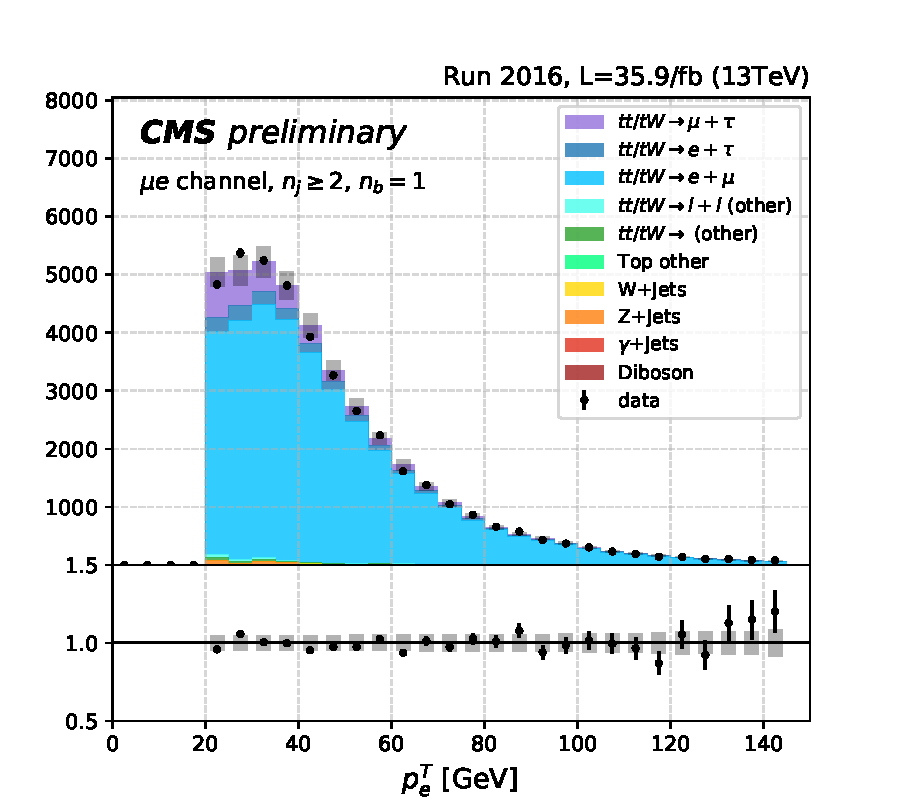
\includegraphics[width=0.24\textwidth]{chapters/Analysis/sectionPlots/figures/kinematics_pickles/emu/1b/emu_1b_lepton2_pt.pdf}
        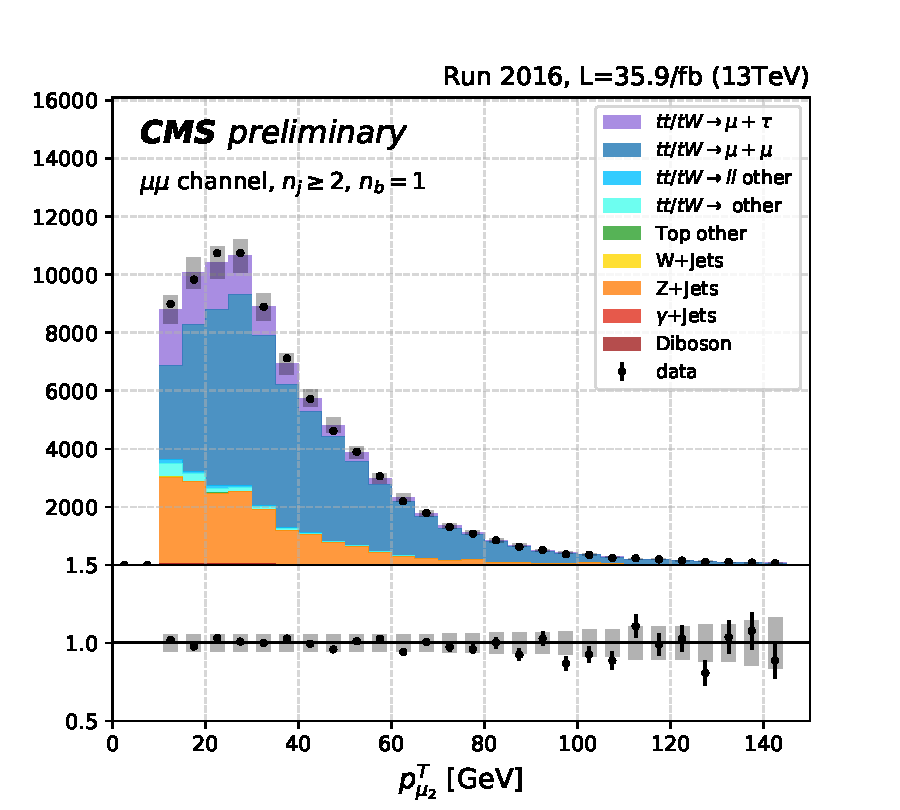
\includegraphics[width=0.24\textwidth]{chapters/Analysis/sectionPlots/figures/kinematics_pickles/mumu/1b/mumu_1b_lepton2_pt.pdf}
        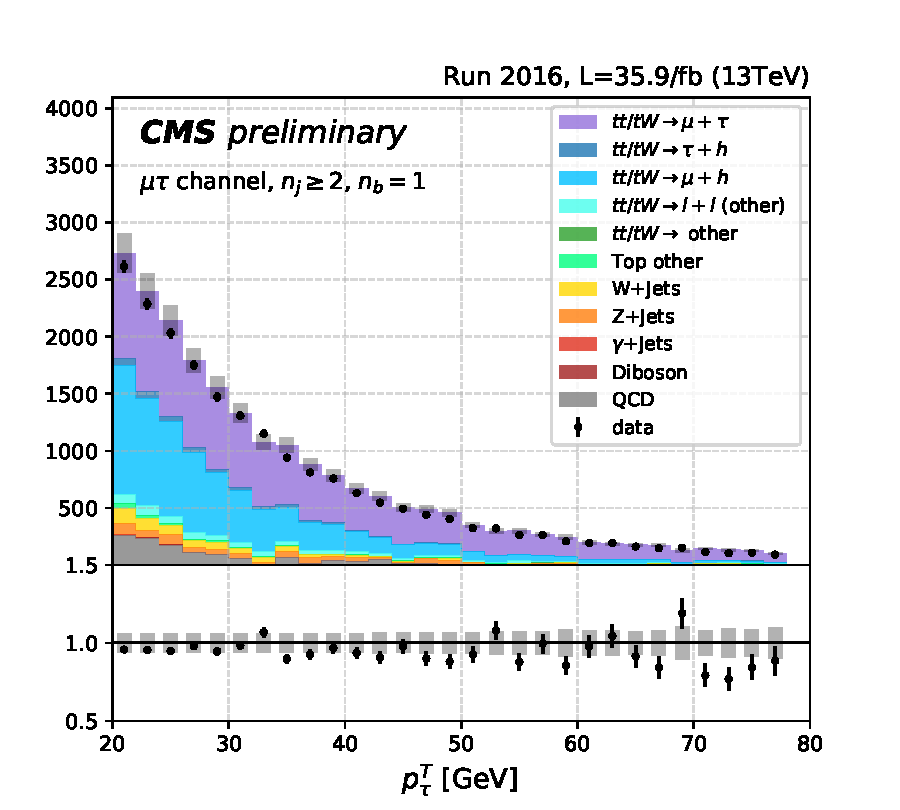
\includegraphics[width=0.24\textwidth]{chapters/Analysis/sectionPlots/figures/kinematics_pickles/mutau/1b/mutau_1b_lepton2_pt.pdf}
        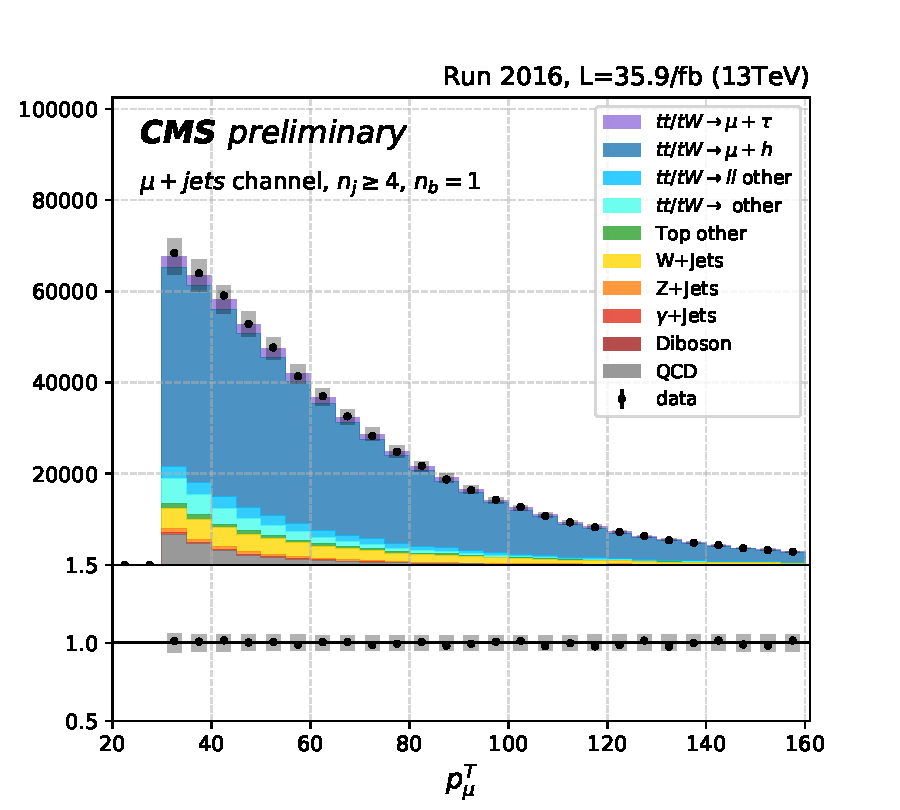
\includegraphics[width=0.24\textwidth]{chapters/Analysis/sectionPlots/figures/kinematics_pickles/mu4j/1b/mu4j_1b_lepton1_pt.pdf}

        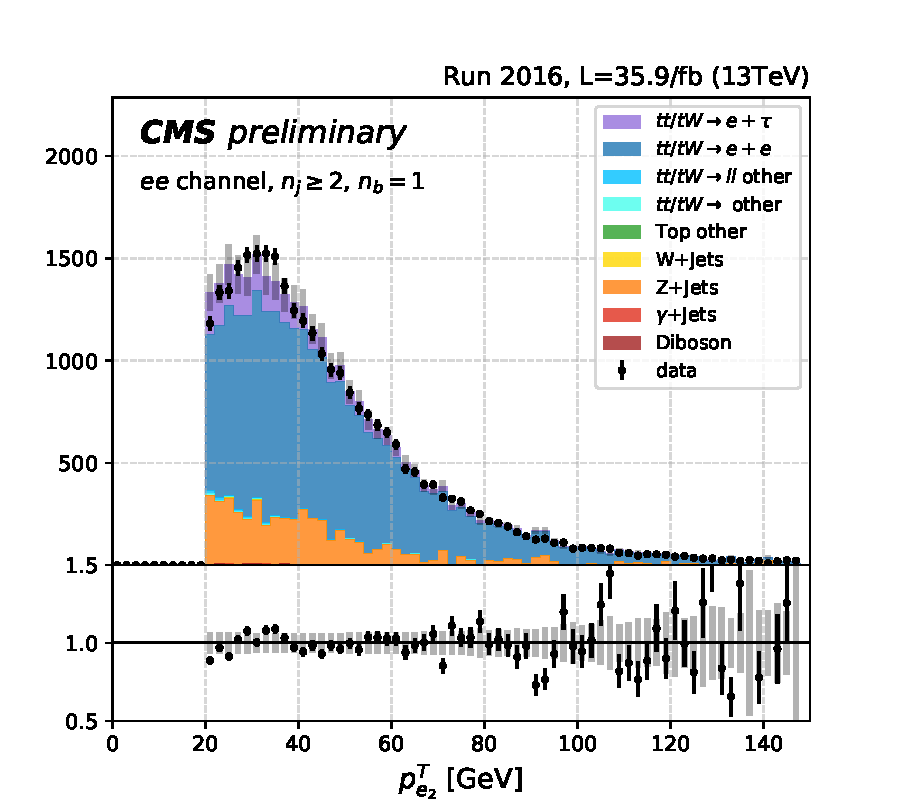
\includegraphics[width=0.24\textwidth]{chapters/Analysis/sectionPlots/figures/kinematics_pickles/ee/1b/ee_1b_lepton2_pt.pdf}
        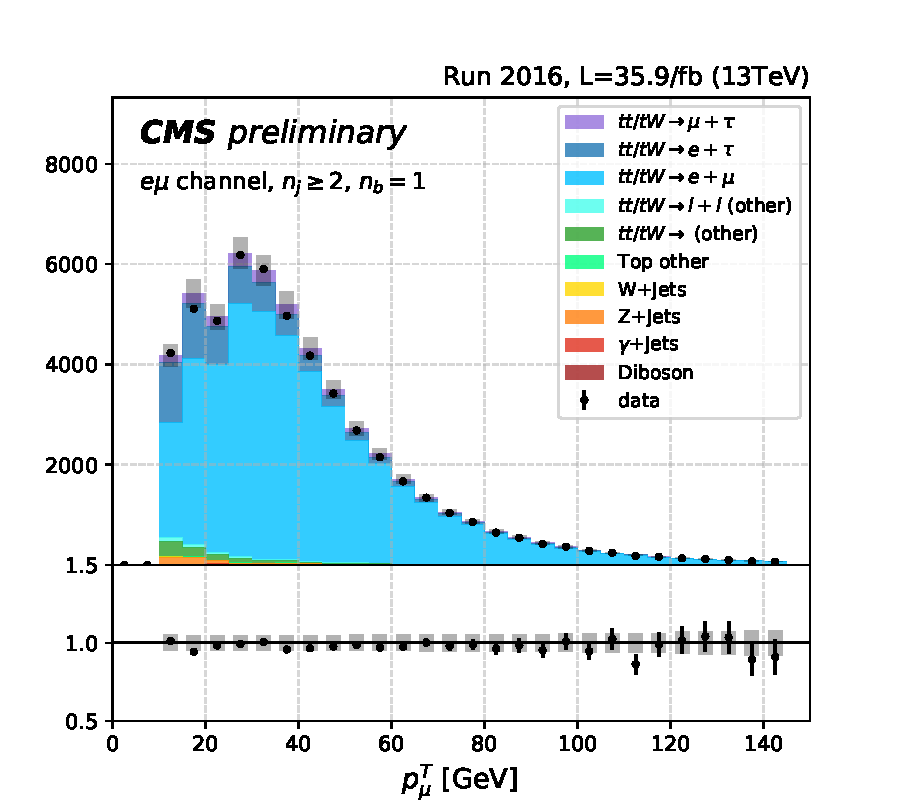
\includegraphics[width=0.24\textwidth]{chapters/Analysis/sectionPlots/figures/kinematics_pickles/emu2/1b/emu2_1b_lepton1_pt.pdf}
        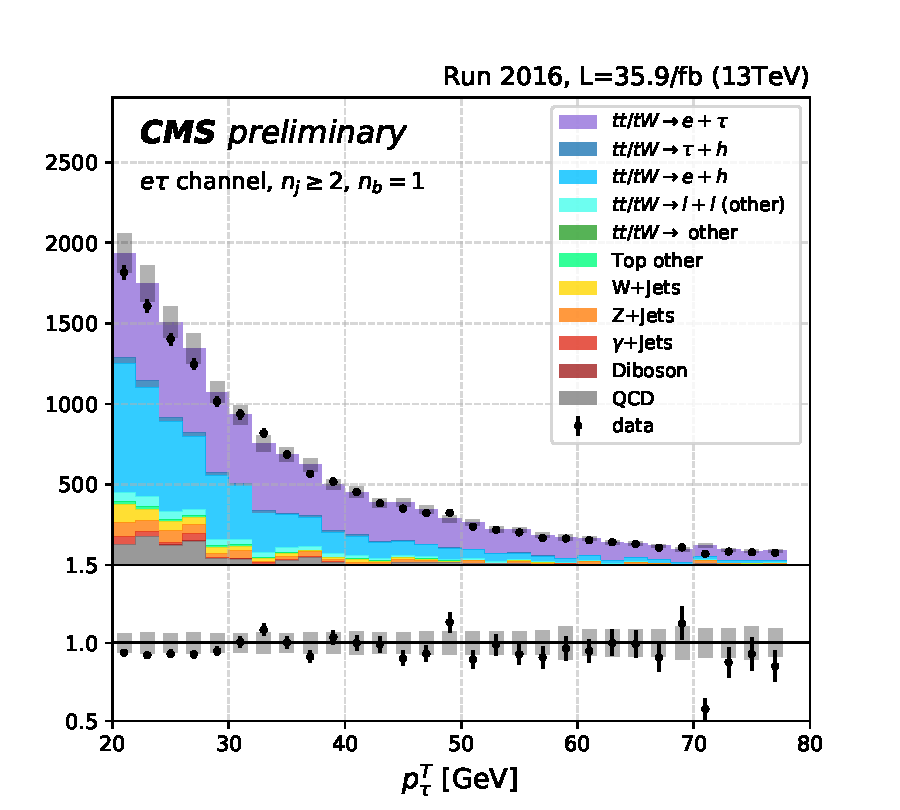
\includegraphics[width=0.24\textwidth]{chapters/Analysis/sectionPlots/figures/kinematics_pickles/etau/1b/etau_1b_lepton2_pt.pdf}
        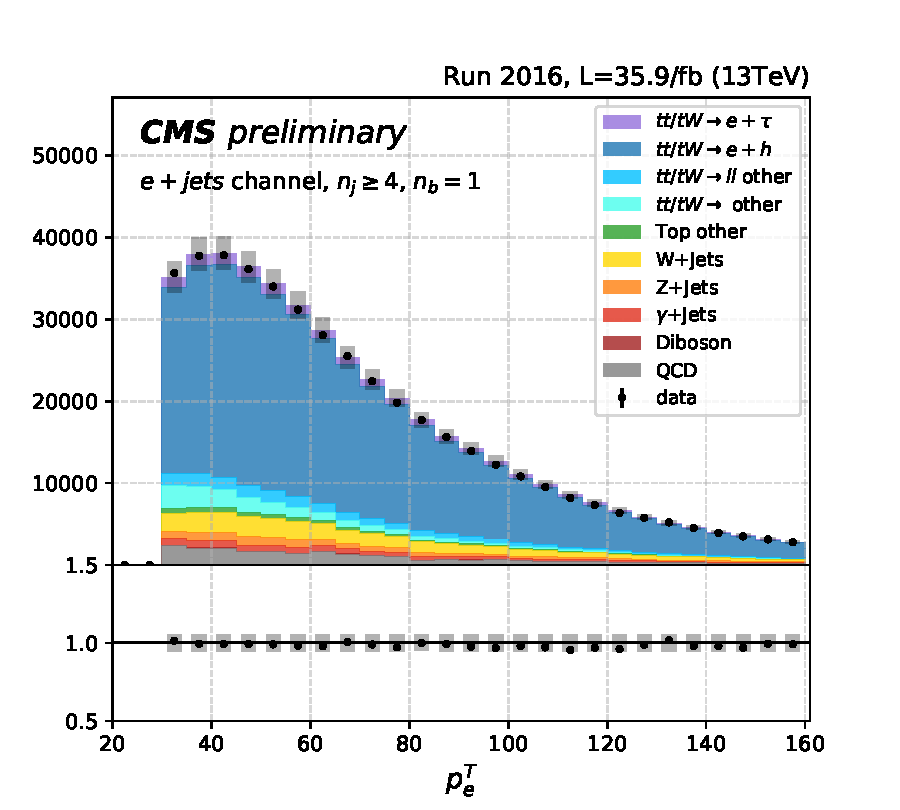
\includegraphics[width=0.24\textwidth]{chapters/Analysis/sectionPlots/figures/kinematics_pickles/e4j/1b/e4j_1b_lepton1_pt.pdf}
    \end{figure}
\end{frame}


% -------------
% new frame
% -------------
\begin{frame}{Event Selection  baseline 2b}
    \begin{figure}
        \centering
        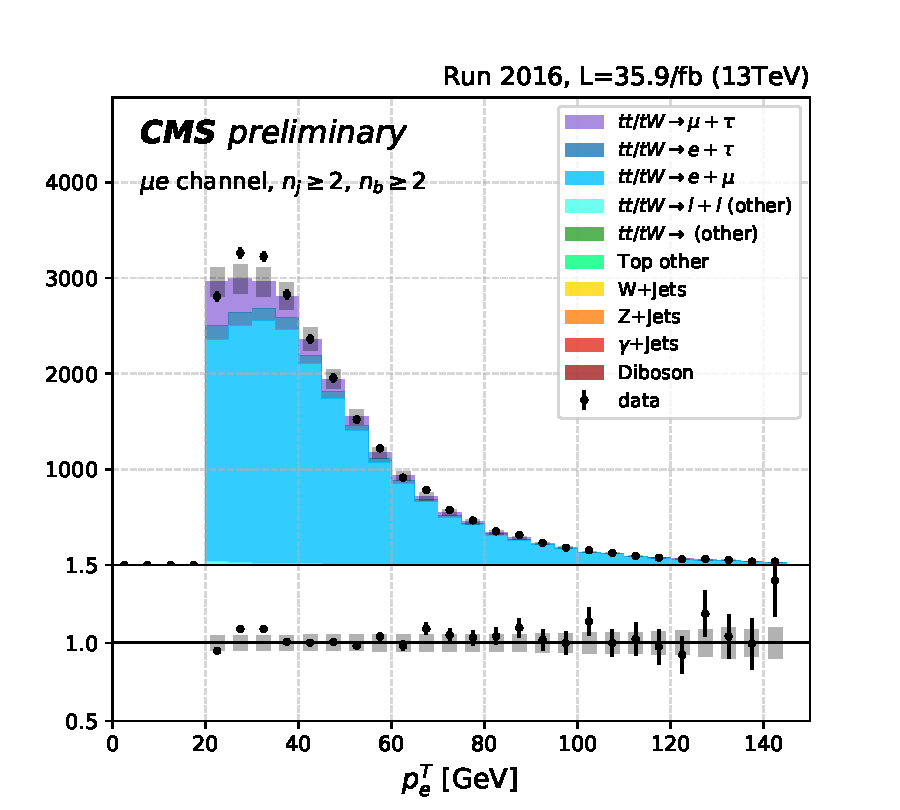
\includegraphics[width=0.24\textwidth]{chapters/Analysis/sectionPlots/figures/kinematics_pickles/emu/2b/emu_2b_lepton2_pt.pdf}
        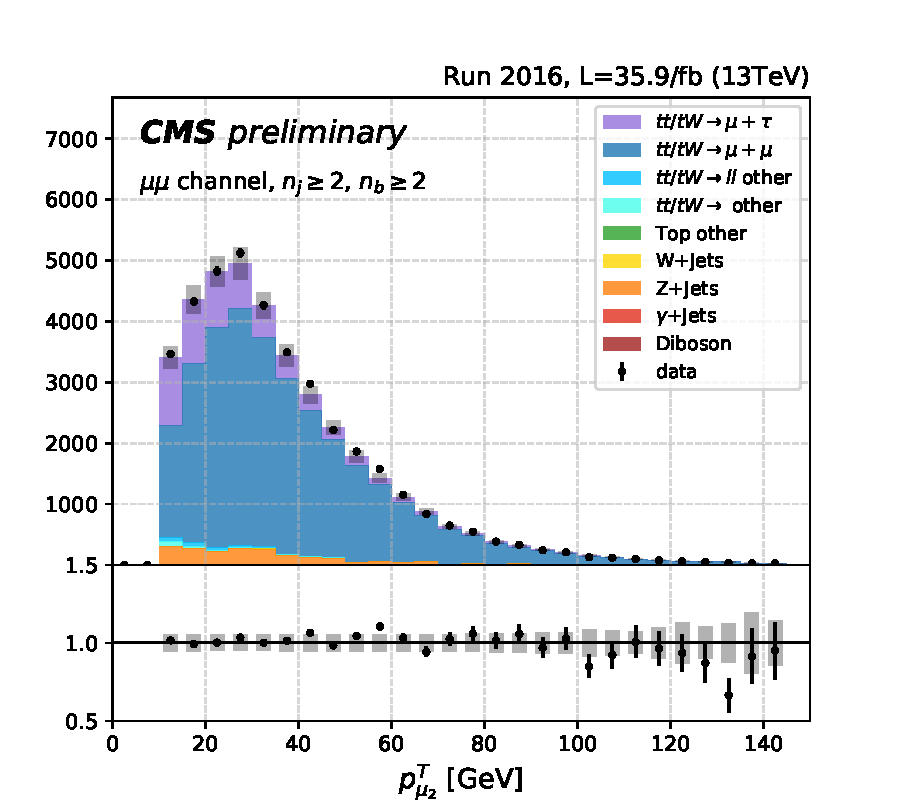
\includegraphics[width=0.24\textwidth]{chapters/Analysis/sectionPlots/figures/kinematics_pickles/mumu/2b/mumu_2b_lepton2_pt.pdf}
        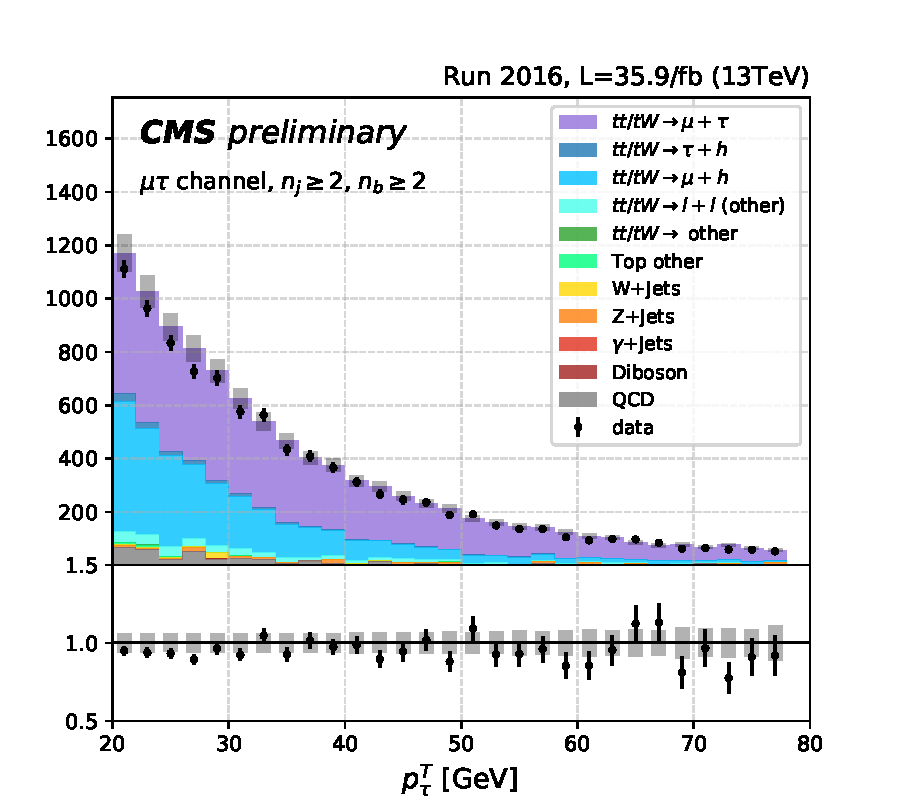
\includegraphics[width=0.24\textwidth]{chapters/Analysis/sectionPlots/figures/kinematics_pickles/mutau/2b/mutau_2b_lepton2_pt.pdf}
        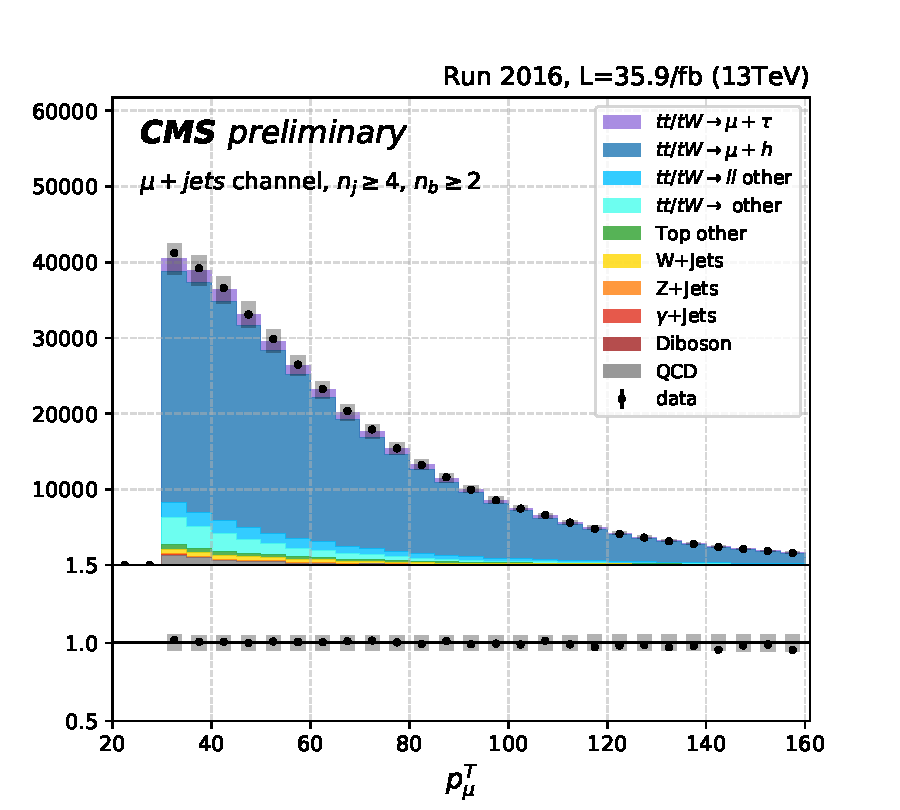
\includegraphics[width=0.24\textwidth]{chapters/Analysis/sectionPlots/figures/kinematics_pickles/mu4j/2b/mu4j_2b_lepton1_pt.pdf}
        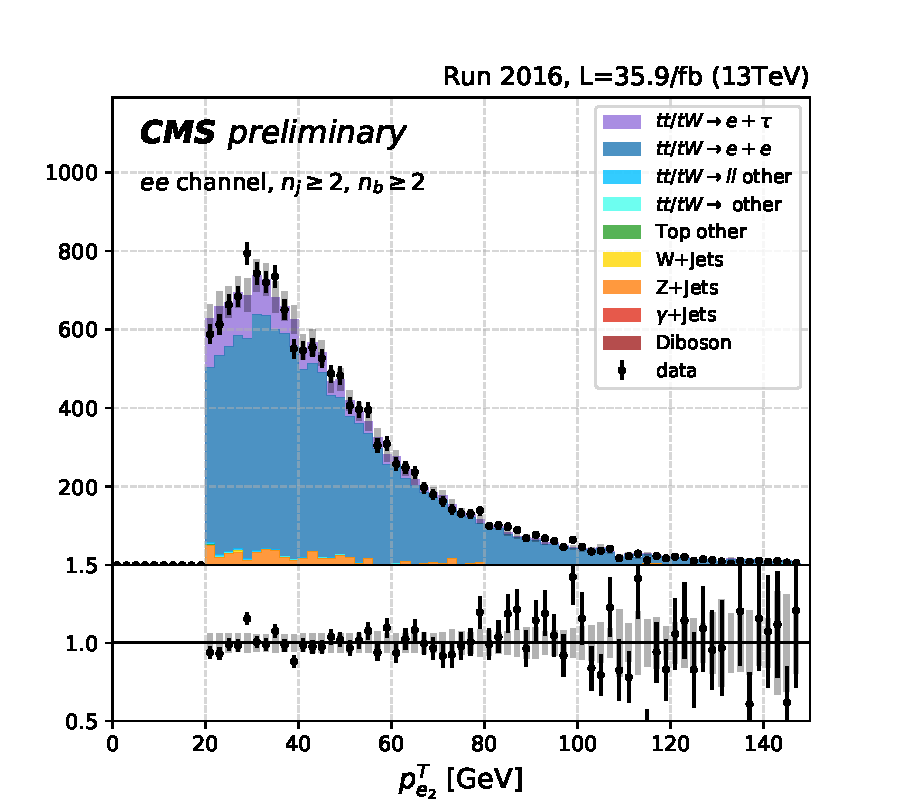
\includegraphics[width=0.24\textwidth]{chapters/Analysis/sectionPlots/figures/kinematics_pickles/ee/2b/ee_2b_lepton2_pt.pdf}
        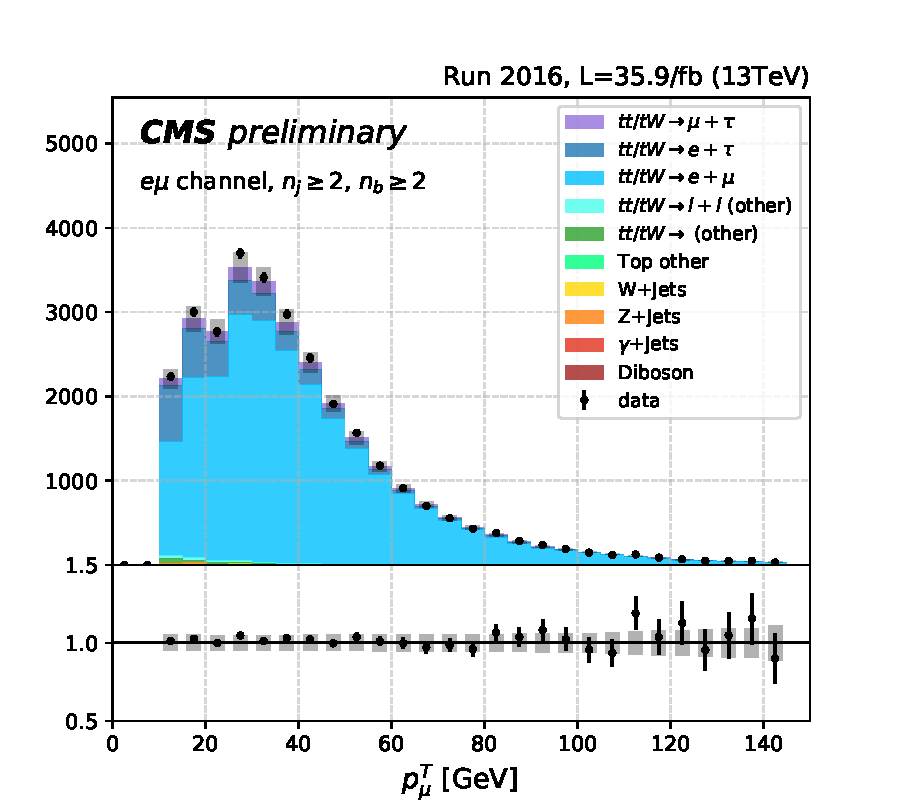
\includegraphics[width=0.24\textwidth]{chapters/Analysis/sectionPlots/figures/kinematics_pickles/emu2/2b/emu2_2b_lepton1_pt.pdf}
        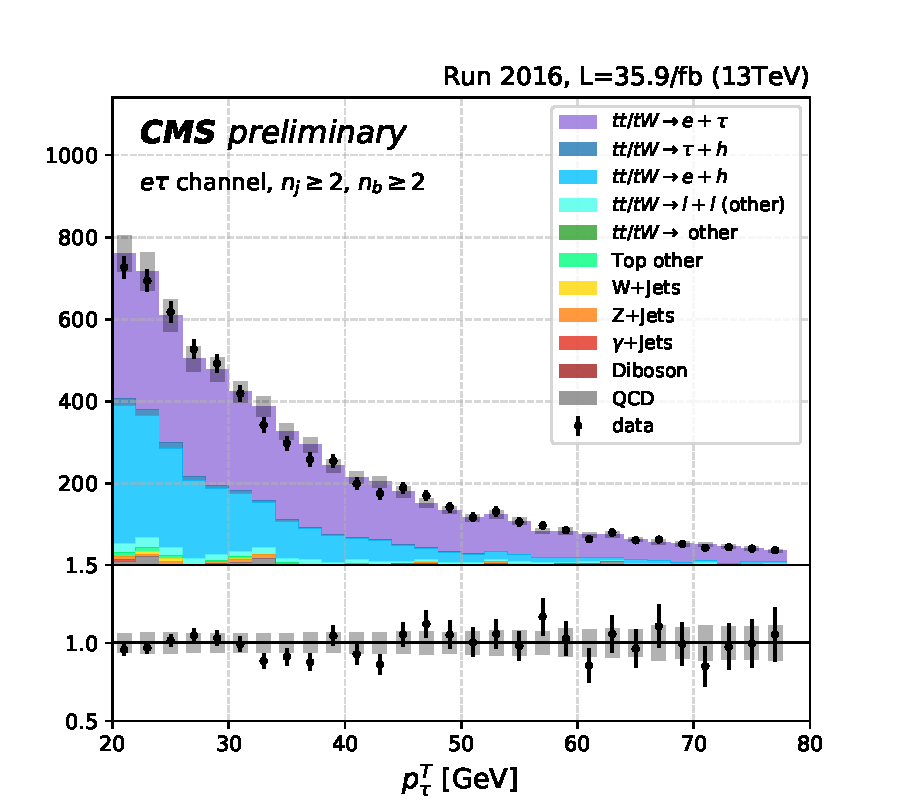
\includegraphics[width=0.24\textwidth]{chapters/Analysis/sectionPlots/figures/kinematics_pickles/etau/2b/etau_2b_lepton2_pt.pdf}
        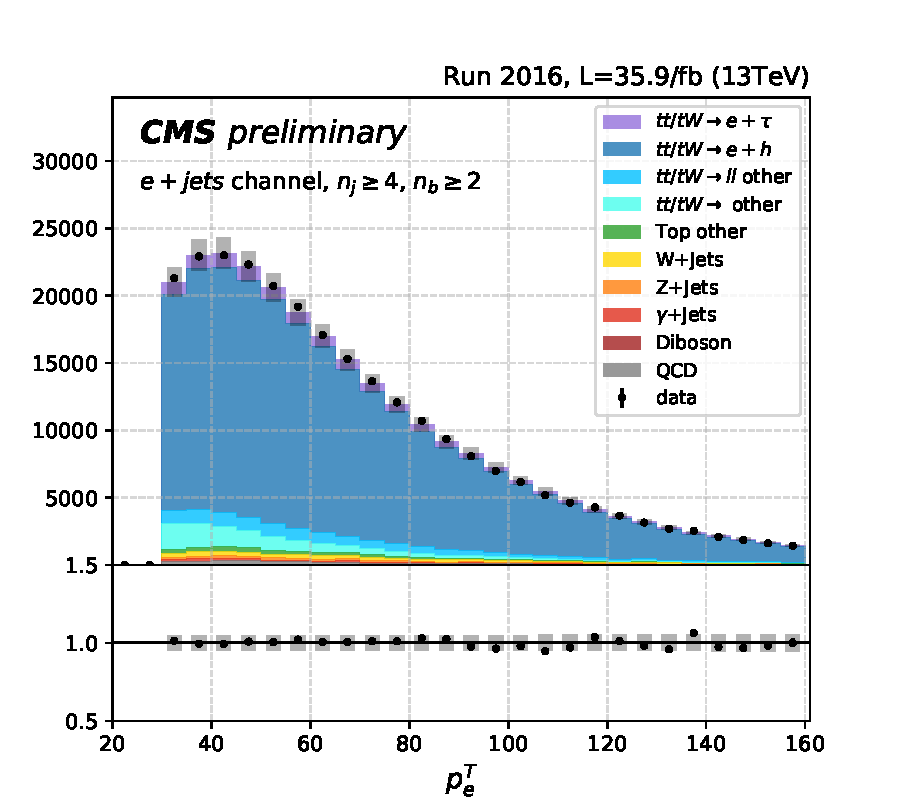
\includegraphics[width=0.24\textwidth]{chapters/Analysis/sectionPlots/figures/kinematics_pickles/e4j/2b/e4j_2b_lepton1_pt.pdf}
    \end{figure}
\end{frame}

% -------------
% new frame
% -------------
\begin{frame}{Event Selection baseline}
    \begin{table}
        \centering
        \setlength{\tabcolsep}{1em}
        \renewcommand{\arraystretch}{2}
        \resizebox{0.96\textwidth}{!}{\begin{sidewaystable}[ht]
    \centering
    \setlength{\tabcolsep}{0.4em}
    \renewcommand{\arraystretch}{1.5}

    \caption{Composition of accepted $t\bar{t}$+$tW$ events, breakdown by 21 WW decay.  Values are in percent.}
    \resizebox{\textwidth}{!}{
    \begin{tabular}{|l|cc|cc|cc|cc|cc|cc|cc|cc|}
    
    
    \hline
    channel & \multicolumn{2}{|c|}{$\mu e$} & \multicolumn{2}{c|}{$\mu\mu$} & \multicolumn{2}{|c|}{$\mu \tau$} & \multicolumn{2}{|c|}{$\mu$+jets} & \multicolumn{2}{|c|}{$ee$} & \multicolumn{2}{|c|}{$e\mu$} & \multicolumn{2}{|c|}{$e \tau$} & \multicolumn{2}{|c|}{$e+jets$} \\
    \hline
    $\rm n_{b tag}$ & $n_b=1$ & $n_b\geq2$ & $n_b=1$ & $n_b\geq2$ & $n_b=1$ & $n_b\geq2$ & $n_b=1$ & $n_b\geq2$ & $n_b=1$ & $n_b\geq2$ & $n_b=1$ & $n_b\geq2$ & $n_b=1$ & $n_b\geq2$ & $n_b=1$ & $n_b\geq2$ \\ 
    \hline
    
    $tt/tW \to ee$                     &   -- &   -- &   -- &   -- &   -- &   -- &   -- &   -- & 87.4 & 87.8 &   -- &   -- &  0.7 &   -- &  3.1 &  3.1 \\ 
    $tt/tW \to \mu\mu$                 &   -- &   -- & 81.6 & 83.0 &   -- &   -- &  1.3 &  1.2 &   -- &   -- &   -- &   -- &   -- &   -- &   -- &   -- \\ 
    $tt/tW \to e\mu$                   & 86.5 & 87.0 &   -- &   -- &  0.8 &  0.5 &  3.3 &  3.3 &   -- &   -- & 82.7 & 84.1 &   -- &   -- &  1.4 &  1.4 \\ 
    $tt/tW \to \tau_{e}\tau_{e}$       &   -- &   -- &   -- &   -- &   -- &   -- &   -- &   -- &   -- &   -- &   -- &   -- &   -- &   -- &   -- &   -- \\ 
    $tt/tW \to \tau_{\mu}\tau_{\mu}$   &   -- &   -- &  0.7 &  0.6 &   -- &   -- &   -- &   -- &   -- &   -- &   -- &   -- &   -- &   -- &   -- &   -- \\ 
    $tt/tW \to \tau_{e}\tau_{\mu}$     &   -- &   -- &   -- &   -- &   -- &   -- &   -- &   -- &   -- &   -- &  0.6 &  0.6 &   -- &   -- &   -- &   -- \\ 
    $tt/tW \to \tau_{e}\tau_{h}$       &   -- &   -- &   -- &   -- &   -- &   -- &   -- &   -- &   -- &   -- &   -- &   -- &  3.1 &  3.2 &   -- &   -- \\ 
    $tt/tW \to \tau_{\mu}\tau_{h}$     &   -- &   -- &   -- &   -- &  3.2 &  3.6 &   -- &   -- &   -- &   -- &   -- &   -- &   -- &   -- &   -- &   -- \\ 
    $tt/tW \to \tau_{h}\tau_{h}$       &   -- &   -- &   -- &   -- &   -- &   -- &   -- &   -- &   -- &   -- &   -- &   -- &   -- &   -- &   -- &   -- \\ 
    $tt/tW \to e\tau_{e}$              &   -- &   -- &   -- &   -- &   -- &   -- &   -- &   -- & 11.7 & 11.5 &   -- &   -- &   -- &   -- &  0.8 &  0.8 \\ 
    $tt/tW \to e\tau_{\mu}$            &  4.1 &  4.0 &   -- &   -- &   -- &   -- &   -- &   -- &   -- &   -- & 11.2 & 11.0 &   -- &   -- &   -- &   -- \\ 
    $tt/tW \to e\tau_{h}$              &   -- &   -- &   -- &   -- &   -- &   -- &   -- &   -- &   -- &   -- &   -- &   -- & 57.5 & 63.6 &  3.4 &  3.6 \\ 
    $tt/tW \to \mu\tau_{e}$            &  8.3 &  8.2 &   -- &   -- &   -- &   -- &  0.6 &  0.7 &   -- &   -- &  3.6 &  3.6 &   -- &   -- &   -- &   -- \\ 
    $tt/tW \to \mu\tau_{\mu}$          &   -- &   -- & 15.7 & 15.8 &   -- &   -- &   -- &   -- &   -- &   -- &   -- &   -- &   -- &   -- &   -- &   -- \\ 
    $tt/tW \to \mu\tau_{h}$            &   -- &   -- &   -- &   -- & 57.4 & 63.6 &  3.4 &  3.6 &   -- &   -- &   -- &   -- &   -- &   -- &   -- &   -- \\ 
    $tt/tW \to eh$                     &   -- &   -- &   -- &   -- &   -- &   -- &   -- &   -- &   -- &   -- &  1.6 &   -- & 35.9 & 30.5 & 85.6 & 85.4 \\ 
    $tt/tW \to \mu h$                  &   -- &   -- &  1.7 &  0.5 & 35.7 & 30.1 & 85.3 & 85.3 &   -- &   -- &   -- &   -- &   -- &   -- &   -- &   -- \\ 
    $tt/tW \to \tau_{e}h$              &   -- &   -- &   -- &   -- &   -- &   -- &   -- &   -- &   -- &   -- &   -- &   -- &  1.9 &  1.6 &  4.8 &  4.7 \\ 
    $tt/tW \to \tau_{\mu}h$            &   -- &   -- &   -- &   -- &  2.1 &  1.6 &  5.0 &  4.9 &   -- &   -- &   -- &   -- &   -- &   -- &   -- &   -- \\ 
    $tt/tW \to \tau_{h}h$              &   -- &   -- &   -- &   -- &   -- &   -- &   -- &   -- &   -- &   -- &   -- &   -- &   -- &   -- &   -- &   -- \\ 
    $tt/tW \to hh$                     &   -- &   -- &   -- &   -- &   -- &   -- &   -- &   -- &   -- &   -- &   -- &   -- &   -- &   -- &   -- &   -- \\ 

    \hline
    \end{tabular}}
    \label{tab:analysis:selection:signal_breakdown}
    
\end{sidewaystable}
}
    \end{table}
\end{frame}


% -------------
% new frame
% -------------
\begin{frame}{Event Selection baseline}
    \begin{table}
        \centering
        \setlength{\tabcolsep}{1em}
        \renewcommand{\arraystretch}{2}
        \resizebox{0.99\textwidth}{!}{


    \begin{tabular}{l|cccccccc|cc}
    \hline
        & QCD & VV  & $\gamma$ & Z & W & t & tW & tt & total & data      \\
    \hline
    
    $\mu e$, $n_b=1$                   &       --$\pm$     -- &     90.3$\pm$    4.2 &      0.9$\pm$    0.9 &    202.7$\pm$   37.6 &     13.4$\pm$    5.1 &      9.5$\pm$    2.6 &   2107.6$\pm$   53.1 &  38871.4$\pm$   87.5 &  41295.8$\pm$  109.2 &  41047.0$\pm$  202.6 \\ 
    $\mu e$, $n_b\geq2$                &       --$\pm$     -- &      5.9$\pm$    1.0 &       --$\pm$     -- &       --$\pm$     -- &      3.1$\pm$    2.2 &      2.3$\pm$    1.6 &    625.7$\pm$   28.9 &  22647.7$\pm$   66.8 &  23270.9$\pm$   74.1 &  23918.0$\pm$  154.7 \\ 
    \hline
    $\mu\mu$, $n_b=1$                  &       --$\pm$     -- &    370.4$\pm$    5.8 &      4.1$\pm$    1.8 &  18046.9$\pm$  455.4 &     52.4$\pm$   11.7 &     55.8$\pm$    6.7 &   3406.2$\pm$   68.8 &  62266.6$\pm$  112.4 &  84202.3$\pm$  474.3 &  84284.0$\pm$  290.3 \\ 
    $\mu\mu$, $n_b\geq2$               &       --$\pm$     -- &     45.8$\pm$    1.5 &      0.0$\pm$    0.0 &   1945.7$\pm$  142.0 &      3.6$\pm$    2.6 &      3.9$\pm$    1.8 &    959.3$\pm$   36.2 &  35685.2$\pm$   85.1 &  38643.4$\pm$  169.6 &  39253.0$\pm$  198.1 \\ 
    \hline
    $\mu\tau$, $n_b=1$                 &   1130.7$\pm$  108.8 &     52.3$\pm$    2.6 &     11.8$\pm$    3.2 &    866.7$\pm$   78.7 &    730.8$\pm$   42.9 &    182.6$\pm$   12.4 &   1291.0$\pm$   41.9 &  18430.0$\pm$   60.6 &  22695.9$\pm$  159.6 &  21621.0$\pm$  147.0 \\ 
    $\mu\tau$, $n_b\geq2$              &    346.6$\pm$   51.5 &      5.5$\pm$    0.7 &      0.9$\pm$    0.8 &    103.6$\pm$   29.6 &     56.9$\pm$   14.4 &     36.8$\pm$    5.6 &    322.6$\pm$   21.0 &   9647.6$\pm$   43.7 &  10520.4$\pm$   78.3 &   9934.0$\pm$   99.7 \\ 
    \hline
    $\mu$+jets, $n_b=1$                &  24300.4$\pm$ 3404.9 &    371.0$\pm$    5.2 &   1501.2$\pm$   67.5 &   7533.2$\pm$  265.9 &  49248.1$\pm$  327.3 &   8484.6$\pm$   85.3 &  24447.8$\pm$  187.0 & 514064.6$\pm$  327.2 & 629950.9$\pm$ 3453.3 & 630704.0$\pm$  794.2 \\ 
    $\mu$+jets, $n_b\geq2$             &   4650.7$\pm$ 1399.5 &     61.4$\pm$    2.0 &    248.3$\pm$   31.8 &   1331.9$\pm$  114.0 &   6524.2$\pm$  118.8 &   5172.2$\pm$   66.7 &  10335.6$\pm$  121.4 & 356185.1$\pm$  272.2 & 384509.5$\pm$ 1442.2 & 385397.0$\pm$  620.8 \\ 
    \hline
    $e e$, $n_b=1$                     &       --$\pm$     -- &    138.2$\pm$    3.6 &      2.8$\pm$    1.2 &   4726.5$\pm$  215.7 &      5.4$\pm$    2.8 &      1.1$\pm$    0.8 &   1382.0$\pm$   42.7 &  23447.3$\pm$   66.9 &  29703.3$\pm$  229.9 &  29491.0$\pm$  171.7 \\ 
    $e e$, $n_b\geq2$                  &       --$\pm$     -- &     16.2$\pm$    0.9 &      0.1$\pm$    0.1 &    500.5$\pm$   67.8 &      3.7$\pm$    2.6 &      2.1$\pm$    1.2 &    371.4$\pm$   22.1 &  13412.7$\pm$   50.7 &  14306.6$\pm$   87.5 &  14334.0$\pm$  119.7 \\ 
    \hline
    $e\mu$, $n_b=1$                    &       --$\pm$     -- &    127.2$\pm$    4.9 &     25.5$\pm$   13.2 &    411.9$\pm$   52.7 &     32.8$\pm$    7.2 &     37.6$\pm$    5.4 &   2917.6$\pm$   62.7 &  49878.6$\pm$   99.2 &  53431.1$\pm$  129.8 &  52362.0$\pm$  228.8 \\ 
    $e\mu$, $n_b\geq2$                 &       --$\pm$     -- &      9.0$\pm$    1.3 &      1.9$\pm$    1.1 &     59.0$\pm$   19.5 &      6.5$\pm$    3.2 &      6.1$\pm$    2.2 &    837.9$\pm$   33.8 &  28374.1$\pm$   74.9 &  29294.5$\pm$   84.6 &  29860.0$\pm$  172.8 \\ 
    \hline
    $e\tau$, $n_b=1$                   &    874.2$\pm$   90.3 &     38.0$\pm$    2.1 &    194.5$\pm$   38.8 &    677.8$\pm$   69.3 &    456.3$\pm$   32.9 &    125.3$\pm$   10.0 &    908.2$\pm$   34.6 &  12884.7$\pm$   49.7 &  16159.1$\pm$  139.0 &  15309.0$\pm$  123.7 \\ 
    $e\tau$, $n_b\geq2$                &     94.2$\pm$   46.3 &      3.0$\pm$    0.4 &     10.0$\pm$    2.9 &     53.4$\pm$   21.3 &     28.7$\pm$    8.5 &     43.4$\pm$    6.0 &    196.1$\pm$   15.9 &   6682.4$\pm$   35.8 &   7111.3$\pm$   65.1 &   7006.0$\pm$   83.7 \\ 
    \hline
    $e$+jets, $n_b=1$                  &  25625.1$\pm$ 2941.3 &    494.9$\pm$    5.1 &  12035.7$\pm$  173.0 &  13119.8$\pm$  323.2 &  34481.3$\pm$  266.1 &   5786.3$\pm$   68.8 &  17454.7$\pm$  154.8 & 360917.6$\pm$  268.5 & 469915.4$\pm$ 2992.9 & 464543.0$\pm$  681.6 \\ 
    $e$+jets, $n_b\geq2$               &   3327.4$\pm$ 1476.4 &     84.5$\pm$    2.0 &   2095.3$\pm$   78.4 &   2520.8$\pm$  138.5 &   4696.3$\pm$   98.0 &   3524.2$\pm$   53.7 &   7616.3$\pm$  102.3 & 249557.0$\pm$  223.4 & 273421.8$\pm$ 1509.3 & 274162.0$\pm$  523.6 \\ 
    \hline

    \end{tabular}}
    \end{table}
\end{frame}


% -------------
% new frame
% -------------
\begin{frame}{Event Selection extended}
    \begin{table}
        \centering
        \setlength{\tabcolsep}{1em}
        \renewcommand{\arraystretch}{2}
        \resizebox{0.7\textwidth}{!}{\begin{tabular}{l|c|c|c c|c}

                                    & $N_j = 0$     & $N_j = 1$      & $N_j = 2$                    & \multicolumn{1}{|c|}{$N_j = 3$}   & $N_j \geq 4$ \\
	\hline
    \multirow{2}{*}{$N_\PQb = 0$}   & \cellcolor{NUpurple10}\textcolor{red}{\cet, \cmt,}  & \cellcolor{NUpurple10}\textcolor{red}{\cet, \cmt,} & \multicolumn{2}{c}{\cellcolor{NUpurple10} \textcolor{red}{\cet, \cmt,} }      & \cellcolor{NUpurple10}\\
                                    & \cellcolor{NUpurple10} \textcolor{blue}{\cem}         & \cellcolor{NUpurple10}\textcolor{blue}{\cem}       & \multicolumn{2}{c}{\cellcolor{NUpurple10} \textcolor{orange}{\cem}}& \cellcolor{NUpurple10}\\
	\hline
    \multirow{3}{*}{$N_\PQb = 1$}   &   & \cellcolor{NUpurple10} \textcolor{orange}{\cet, \cmt, \cem } & \cet, \cmt   & \multicolumn{2}{!{\color{OliveGreen}\vrule width 2pt}c}{\cet, \cmt} \\
	\cline{3-6}
                                    & \multicolumn{2}{c|}{} & \multicolumn{3}{c}{ \cee, \cmm, \cem}                                        \\
	\cline{4-6}
                                    & \multicolumn{4}{c|}{} & \ceh, \cmh \\
	\hline

    \multirow{3}{*}{$N_\PQb \geq 2$} & \multicolumn{2}{c|}{} & \cet, \cmt & \multicolumn{2}{!{\color{OliveGreen}\vrule width 2pt}c}{\cet, \cmt} \\
	\cline{4-6}
                                    & \multicolumn{2}{c|}{} & \multicolumn{3}{c}{$\cee, \cmm, \cem$}                                        \\
	\cline{4-6}
                                    & \multicolumn{4}{c|}{} & \ceh, \cmh \\
	\hline
\end{tabular}}
    \end{table}
\end{frame}




% -------------
% new frame
% -------------
\begin{frame}{Event Selection  baseline 2b}
    \begin{tcolorbox}[colframe=red,colback=white]{$Z\to \PGtl \PGth$}
        \begin{center}
        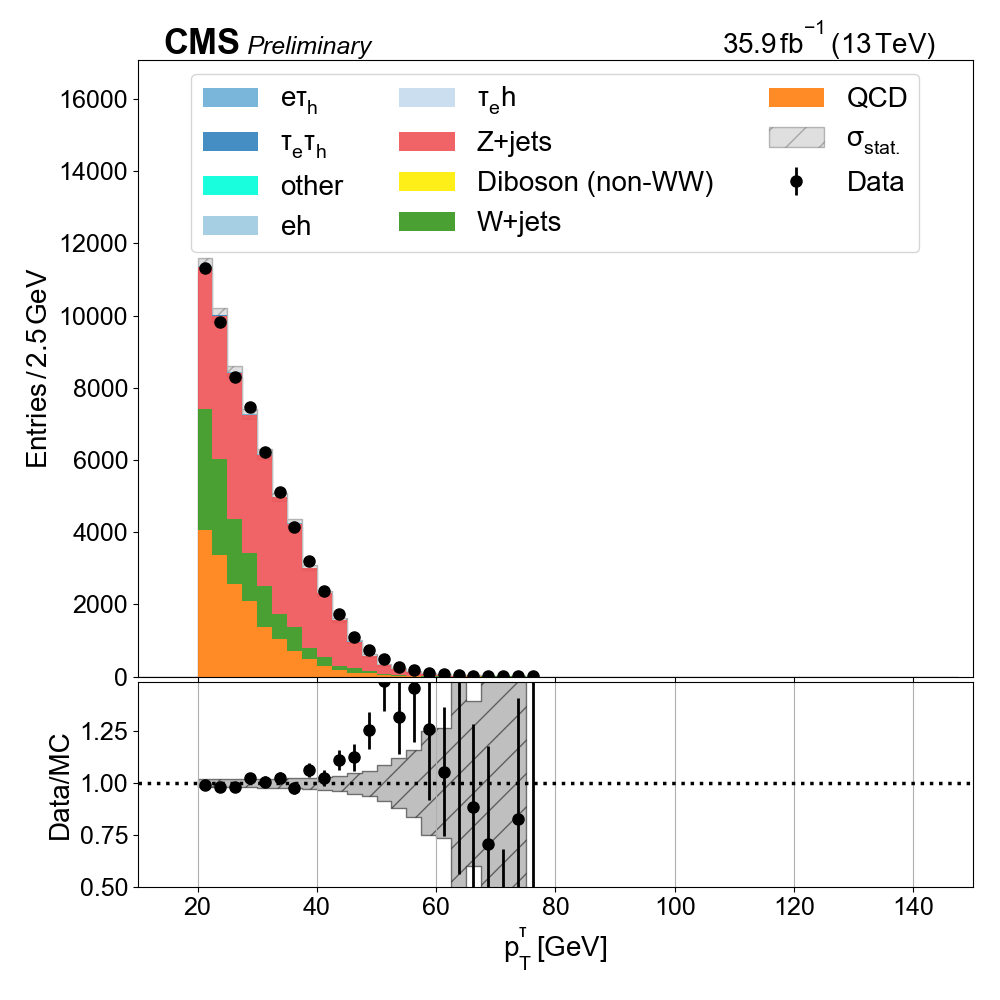
\includegraphics[width=0.3\textwidth]{chapters/Analysis/sectionPlots/figures/data_mc_overlays/etau_2016_cat_eq0_eq0_signal_linear_lepton_lepton2_pt.png}
        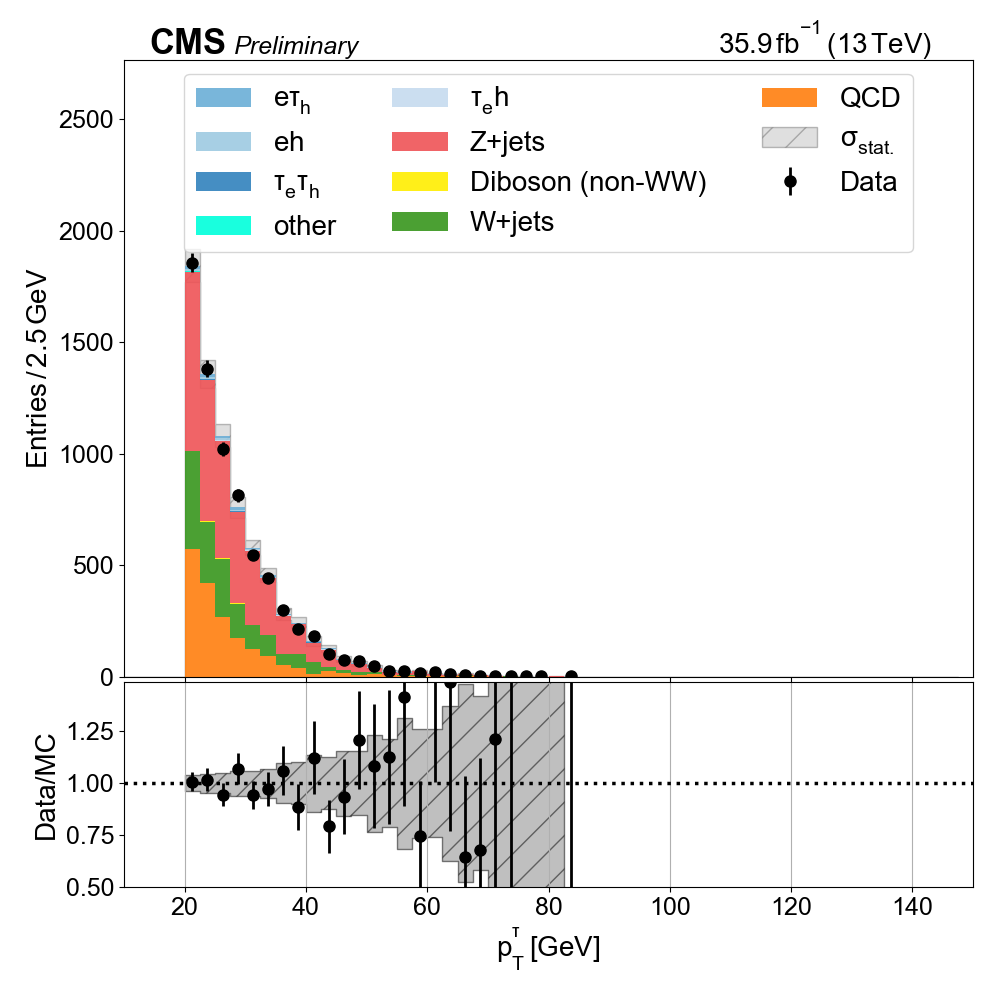
\includegraphics[width=0.3\textwidth]{chapters/Analysis/sectionPlots/figures/data_mc_overlays/etau_2016_cat_eq1_eq0_signal_linear_lepton_lepton2_pt.png}
        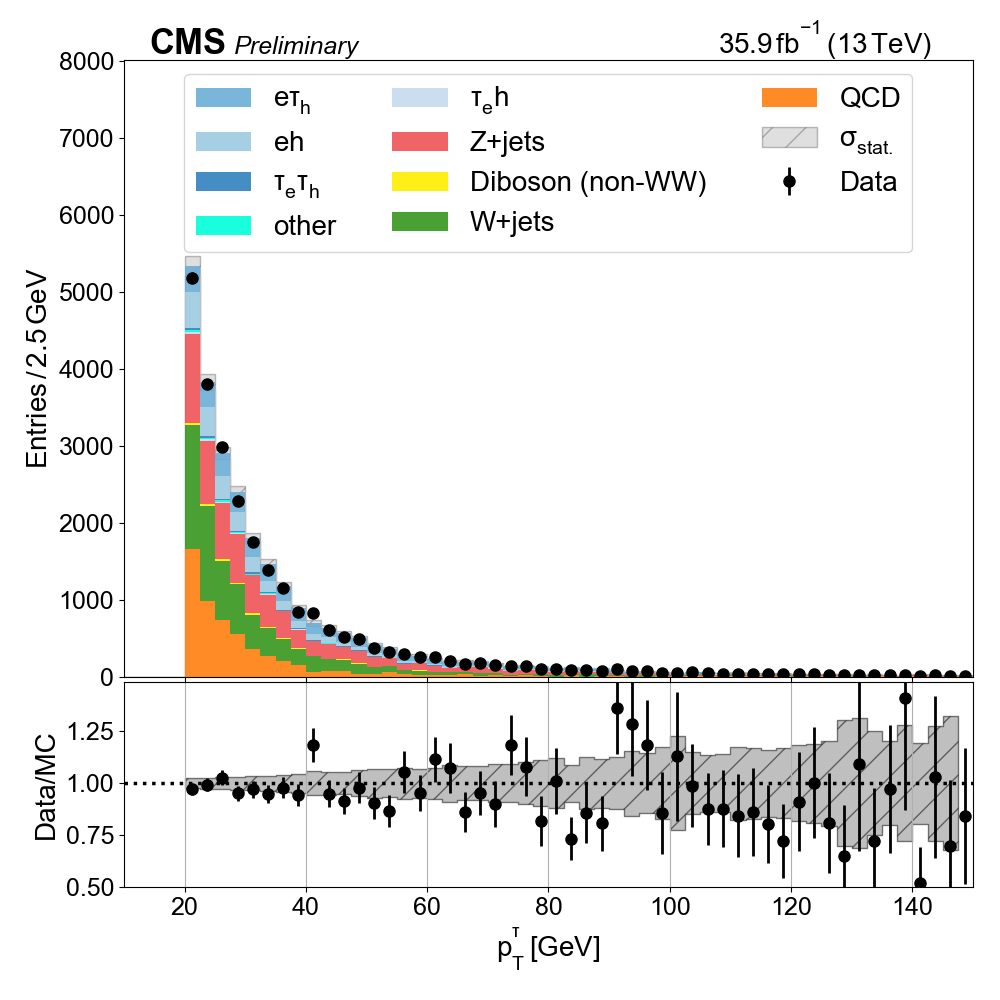
\includegraphics[width=0.3\textwidth]{chapters/Analysis/sectionPlots/figures/data_mc_overlays/etau_2016_cat_gt2_eq0_signal_linear_lepton_lepton2_pt.png}
        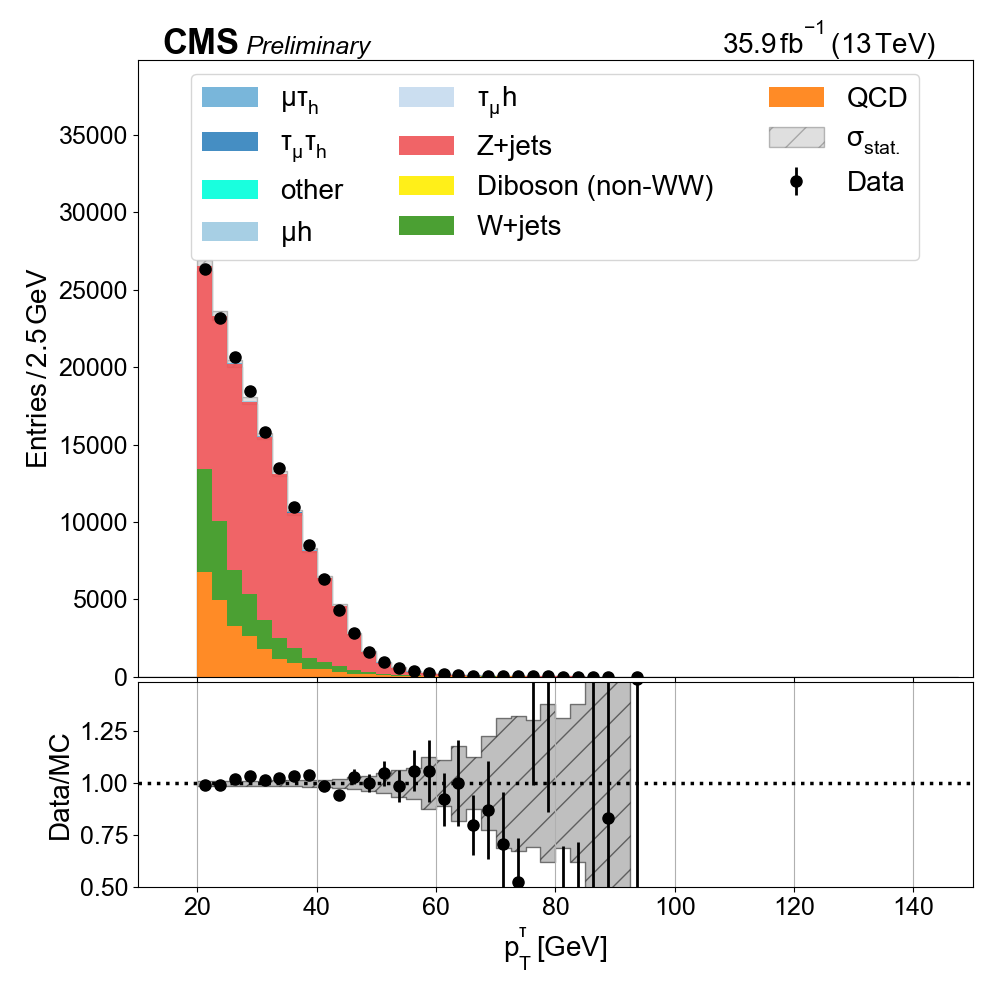
\includegraphics[width=0.3\textwidth]{chapters/Analysis/sectionPlots/figures/data_mc_overlays/mutau_2016_cat_eq0_eq0_signal_linear_lepton_lepton2_pt.png}
        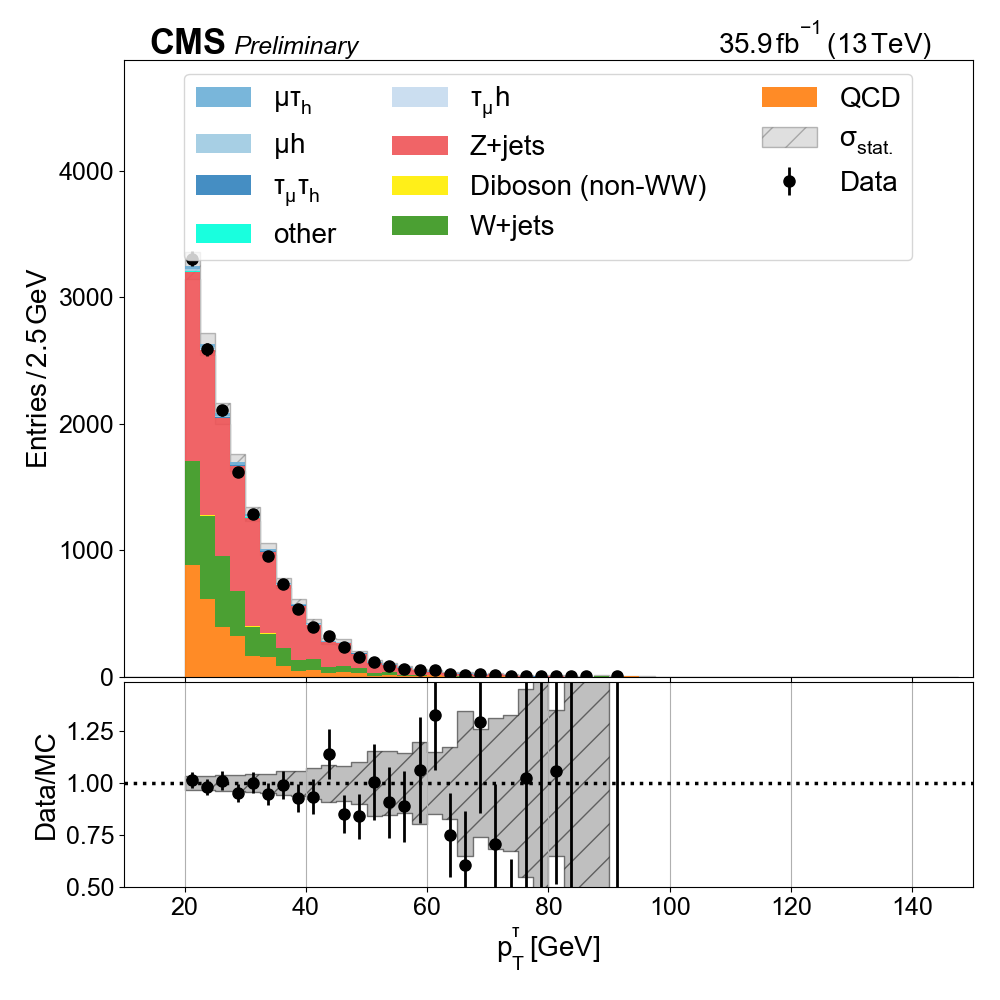
\includegraphics[width=0.3\textwidth]{chapters/Analysis/sectionPlots/figures/data_mc_overlays/mutau_2016_cat_eq1_eq0_signal_linear_lepton_lepton2_pt.png}
        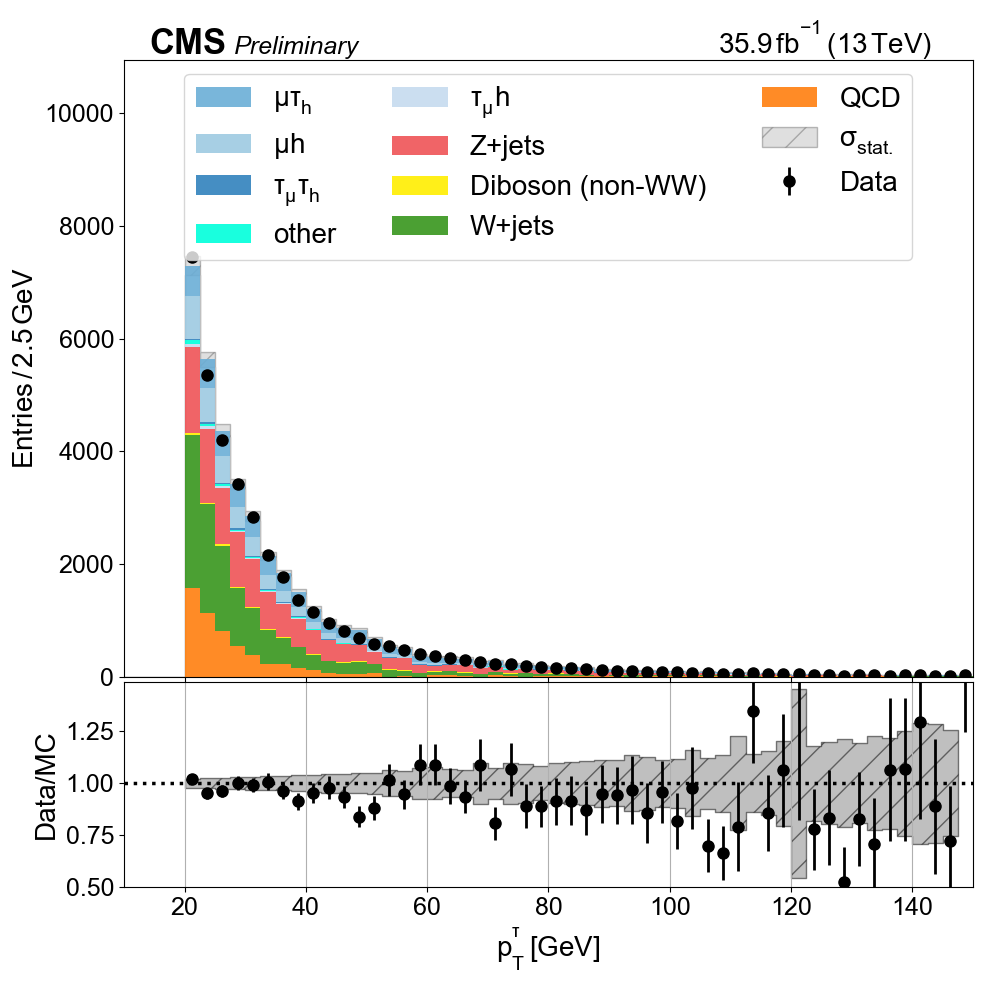
\includegraphics[width=0.3\textwidth]{chapters/Analysis/sectionPlots/figures/data_mc_overlays/mutau_2016_cat_gt2_eq0_signal_linear_lepton_lepton2_pt.png}        
        \end{center}
    \end{tcolorbox}
\end{frame}

% -------------
% new frame
% -------------
\begin{frame}{Event Selection  baseline 2b}
    \begin{tcolorbox}[colframe=blue,colback=white]{$\WW \to \Pe \PGm$}
        \begin{center}
        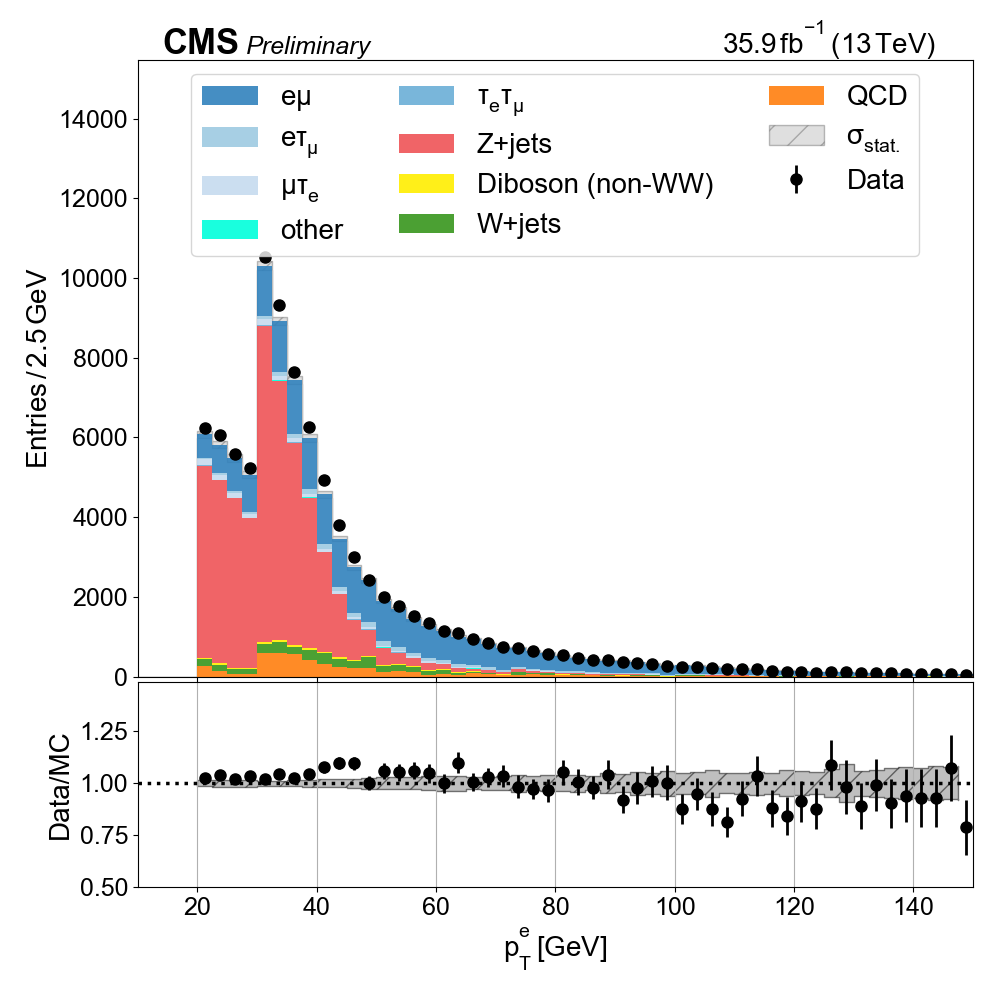
\includegraphics[width=0.30\textwidth]{chapters/Analysis/sectionPlots/figures/data_mc_overlays/emu_2016_cat_eq0_eq0_a_signal_linear_lepton_lepton2_pt.png}
        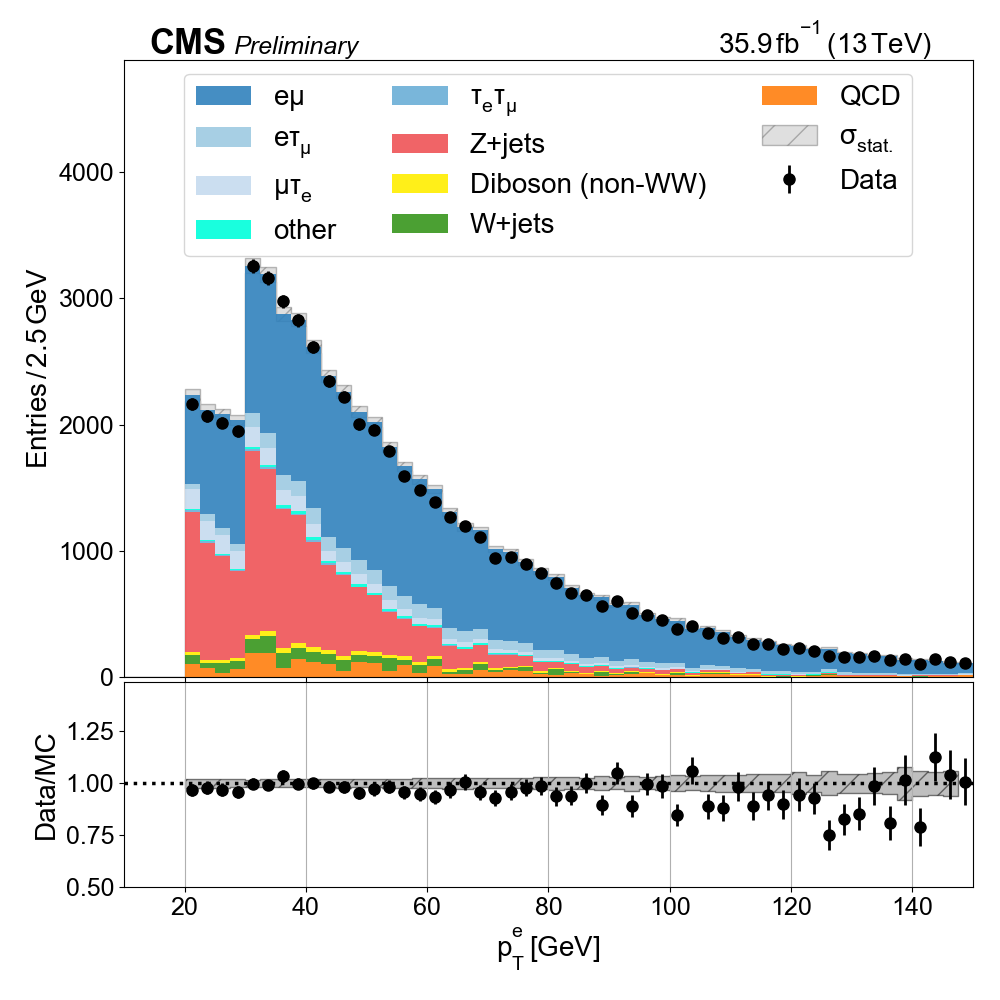
\includegraphics[width=0.30\textwidth]{chapters/Analysis/sectionPlots/figures/data_mc_overlays/emu_2016_cat_eq1_eq0_a_signal_linear_lepton_lepton2_pt.png}
        \end{center}
    \end{tcolorbox}
\end{frame}

% -------------
% new frame
% -------------
\begin{frame}{Event Selection  baseline 2b}
    \begin{tcolorbox}[colframe=orange,colback=white]{$\ttbar$ extra}
        \begin{center}
        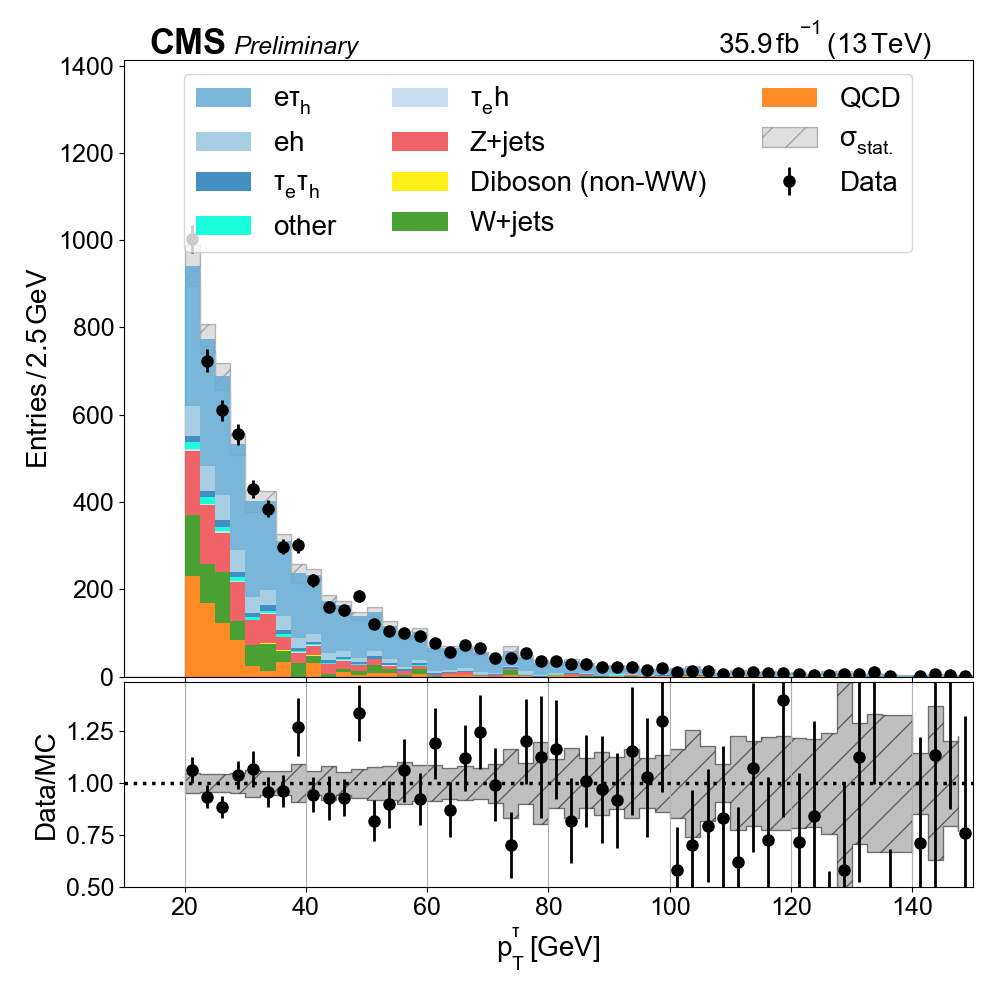
\includegraphics[width=0.30\textwidth]{chapters/Analysis/sectionPlots/figures/data_mc_overlays/etau_2016_cat_eq1_eq1_signal_linear_lepton_lepton2_pt.png}
        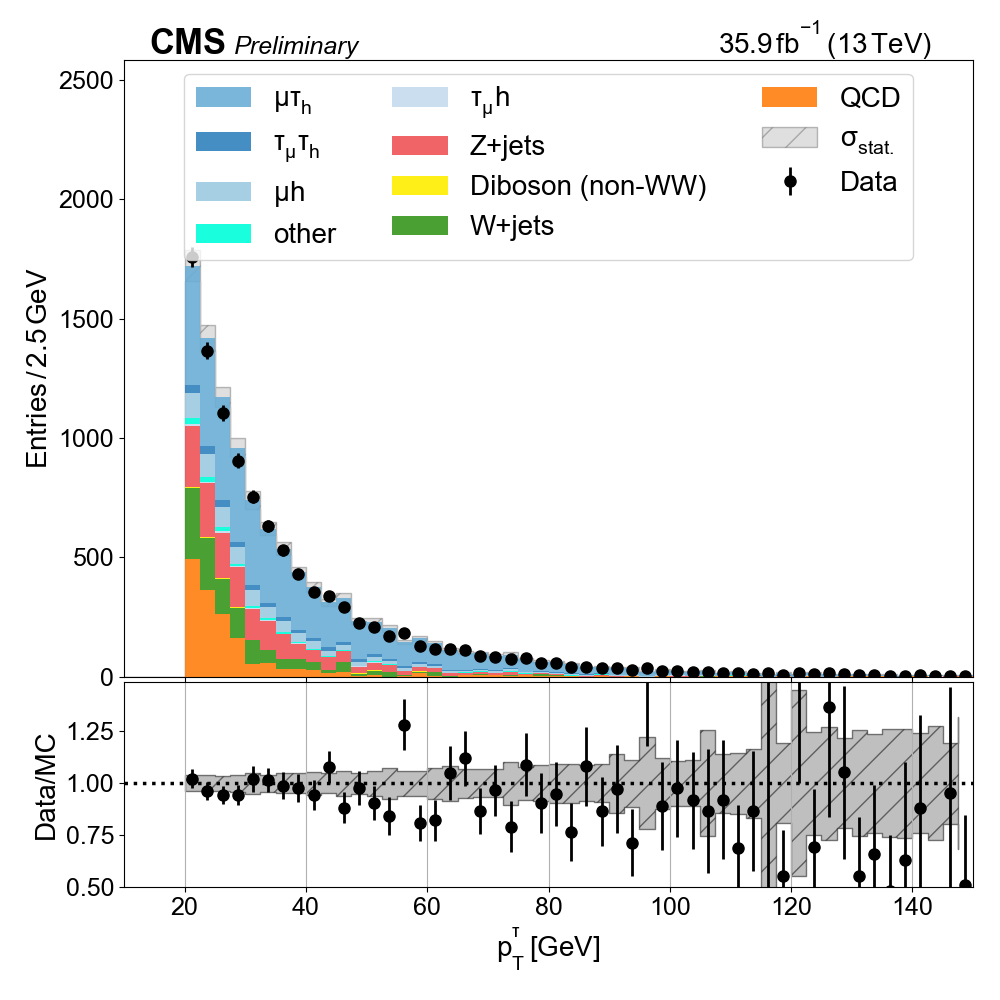
\includegraphics[width=0.30\textwidth]{chapters/Analysis/sectionPlots/figures/data_mc_overlays/mutau_2016_cat_eq1_eq1_signal_linear_lepton_lepton2_pt.png}
        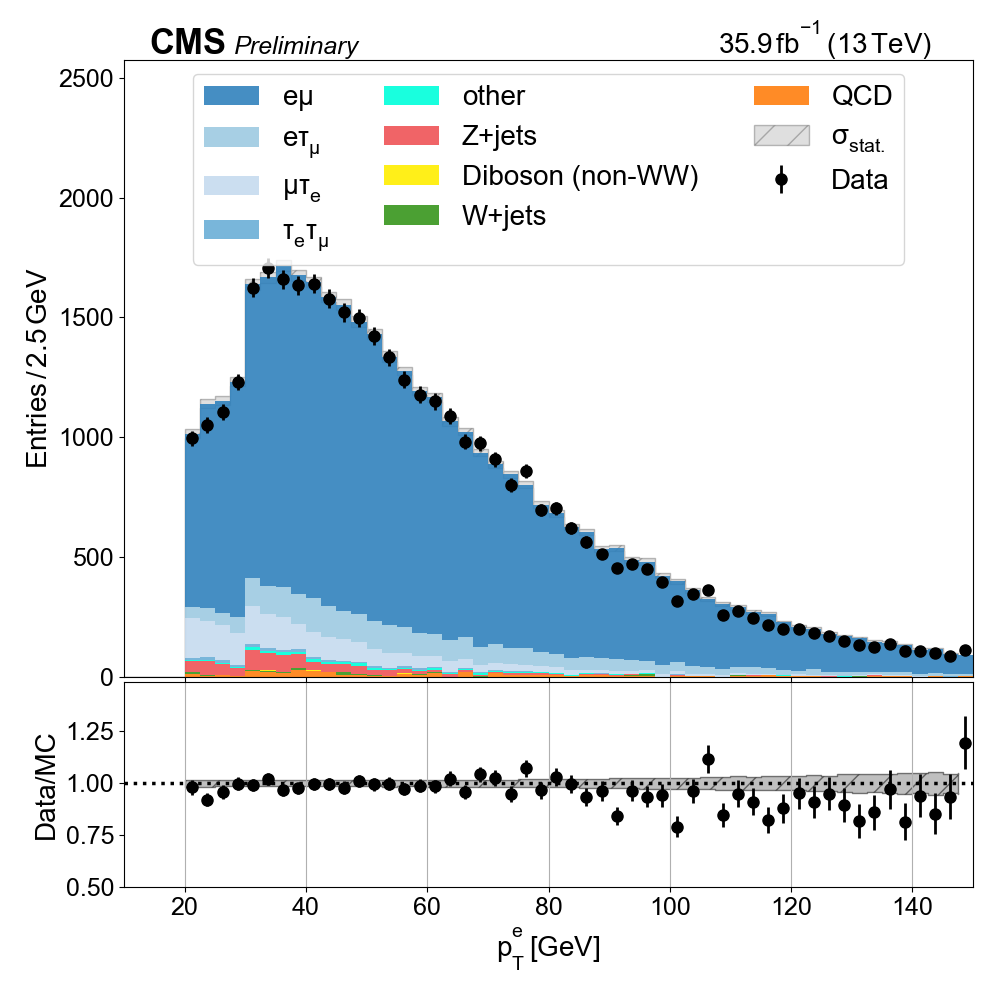
\includegraphics[width=0.30\textwidth]{chapters/Analysis/sectionPlots/figures/data_mc_overlays/emu_2016_cat_eq1_eq1_a_signal_linear_lepton_lepton2_pt.png}
        \end{center}
    \end{tcolorbox}
\end{frame}


% -------------
% new frame
% -------------
\begin{frame}{Event Selection extended}
    \begin{table}
        \centering
        \setlength{\tabcolsep}{1em}
        \renewcommand{\arraystretch}{2}
        \resizebox{0.99\textwidth}{!}{\begin{sidewaystable}
    \centering
    \setlength{\tabcolsep}{0.2em}
    \renewcommand{\arraystretch}{1.5}
    
    \caption{Estimates of the yields for various processes in the $ee$,
    $\mu\mu$, $e\mu$ and semileptonic final states broken down by the
    number of b tags.  The estimate of the expected yield is compared to
    the yield observed from data.  Uncertainties are statistical plus
    variation from luminosity and normalization uncertainties.}
    
    
    \resizebox{\textwidth}{!}{
        \begin{tabular}{l|ccccccc|cc}
        \hline
                                           & QCD                  & Diboson (non-WW)   & WW                 & Z                      & W & tW                   & $\rm t\bar{t}$         & Expected               & Observed \\
        \hline
        \multicolumn{10}{l}{$ee$}         \\
        \hline
        $N_{j} \geq 2, N_{b} = 0$          & --                   & $1014.2 \pm 104.7$ & $804.9 \pm 46.8$   & $55026.7 \pm 5713.1$   & $175.2 \pm 25.0$     & $854.4 \pm 58.0$     & $10865.1 \pm 609.1$    & $68740.4 \pm 5747.0$   & $68657$  \\
        $N_{j} \geq 2, N_{b} = 1$          & --                   & $119.6 \pm 12.4$   & $51.2 \pm 4.3$     & $5207.9 \pm 579.0$     & $10.1 \pm 4.8$       & $1415.3 \pm 89.8$    & $24815.2 \pm 1388.9$   & $31619.1 \pm 1507.5$   & $30332$  \\
        $N_{j} \geq 2, N_{b} \geq 2$       & --                   & $17.2 \pm 1.8$     & $3.3 \pm 0.8$      & $504.9 \pm 86.2$       & $5.2 \pm 3.7$        & $384.5 \pm 30.8$     & $14121.1 \pm 791.1$    & $15036.2 \pm 796.4$    & $14646$  \\
        \hline
        \multicolumn{10}{l}{$\mu\mu$}     \\
        \hline
        $N_{j} \geq 2, N_{b} = 0$          & --                   & $2628.2 \pm 271.0$ & $1944.1 \pm 110.6$ & $194725.6 \pm 20123.0$ & $455.9 \pm 43.1$     & $2081.2 \pm 127.6$   & $28399.5 \pm 1589.3$   & $230234.5 \pm 20188.2$ & $238485$ \\
        $N_{j} \geq 2, N_{b} = 1$          & --                   & $324.9 \pm 33.6$   & $128.4 \pm 8.9$    & $19150.5 \pm 2023.9$   & $80.0 \pm 16.4$      & $3469.2 \pm 205.5$   & $64582.6 \pm 3612.0$   & $87735.6 \pm 4145.7$   & $86354$  \\
        $N_{j} \geq 2, N_{b} \geq 2$       & --                   & $48.3 \pm 5.0$     & $5.8 \pm 1.1$      & $2028.9 \pm 253.5$     & $5.3 \pm 3.8$        & $976.6 \pm 65.4$     & $36916.5 \pm 2065.4$   & $39981.3 \pm 2082.0$   & $40011$  \\
        \hline
        \multicolumn{10}{l}{$e\mu$}         \\
        \hline
        $N_{j} = 0, N_{b} = 0$       & $4264.9 \pm 285.7$ & $748.9 \pm 77.6$ & $17566.8 \pm 983.8$ & $49838.9 \pm 5152.2$ & $3713.1 \pm 262.4$ & $3305.7 \pm 196.0$ & $9606.0 \pm 538.7$   & $89044.3 \pm 5291.3$ & $90784$  \\
        $N_{j} = 1, N_{b} = 0$       & $1907.5 \pm 164.2$ & $774.1 \pm 80.2$ & $7384.9 \pm 414.6$  & $13584.5 \pm 1424.6$ & $1700.9 \pm 131.7$ & $5413.8 \pm 313.9$ & $25755.0 \pm 1441.5$ & $56520.8 \pm 2104.4$ & $55427$  \\
        $N_{j} = 1, N_{b} = 1$       & $279.7 \pm 42.4$   & $21.2 \pm 2.5$   & $173.9 \pm 11.4$    & $712.9 \pm 98.8$     & $95.5 \pm 18.5$    & $6330.4 \pm 365.2$ & $32341.1 \pm 1809.6$ & $39954.7 \pm 1849.4$ & $39021$  \\
        $N_{j} \geq 2, N_{b} = 0$    & $737.0 \pm 95.6$   & $582.4 \pm 60.4$ & $2780.4 \pm 157.3$  & $5280.2 \pm 574.9$   & $710.3 \pm 60.7$   & $3117.8 \pm 185.5$ & $40246.2 \pm 2251.5$ & $53454.4 \pm 2340.0$ & $50301$  \\
        $N_{j} \geq 2, N_{b} = 1$    & $403.7 \pm 60.4$   & $47.0 \pm 5.2$   & $185.6 \pm 12.1$    & $605.3 \pm 89.0$     & $64.9 \pm 13.2$    & $5127.5 \pm 298.0$ & $91534.6 \pm 5118.7$ & $97968.5 \pm 5128.5$ & $93440$  \\
        $N_{j} \geq 2, N_{b} \geq 2$ & $203.0 \pm 29.2$   & $4.2 \pm 0.6$    & $13.1 \pm 1.8$      & $61.8 \pm 23.9$      & $14.7 \pm 6.1$     & $1510.7 \pm 95.4$  & $52401.6 \pm 2931.1$ & $54209.1 \pm 2932.9$ & $53859$  \\
        \hline
        \multicolumn{10}{l}{$e$ + jets}   \\
        \hline
        $N_{j} \geq 2, N_{b} = 1$          & $13189.3 \pm 740.4$  & $578.8 \pm 59.7$   & $65.2 \pm 5.2$     & $13637.7 \pm 1442.7$   & $46769.4 \pm 2637.7$ & $17675.4 \pm 999.7$  & $371951.7 \pm 20794.5$ & $463867.6 \pm 21047.6$ & $468222$ \\
        $N_{j} \geq 2, N_{b} \geq 2$       & $4665.8 \pm 263.9$   & $104.4 \pm 10.8$   & $7.1 \pm 1.3$      & $2367.0 \pm 279.5$     & $6359.5 \pm 378.1$   & $7591.6 \pm 435.9$   & $256643.9 \pm 14348.6$ & $277739.3 \pm 14365.3$ & $276116$ \\
        \hline
        \multicolumn{10}{l}{$\mu$ + jets} \\
        \hline
        $N_{j} \geq 2, N_{b} = 1$          & $42676.6 \pm 2389.3$ & $458.4 \pm 47.3$   & $90.1 \pm 6.7$     & $10504.3 \pm 1123.2$   & $71625.7 \pm 4028.2$ & $26161.6 \pm 1474.4$ & $572088.3 \pm 31982.5$ & $723605.0 \pm 32376.7$ & $710650$ \\
        $N_{j} \geq 2, N_{b} \geq 2$       & $13244.3 \pm 743.9$  & $82.9 \pm 8.6$     & $9.0 \pm 1.5$      & $1738.4 \pm 219.6$     & $9522.0 \pm 555.9$   & $11251.4 \pm 640.8$  & $397617.9 \pm 22229.3$ & $433465.8 \pm 22259.0$ & $429861$ \\
        \hline
    \end{tabular}}

    \label{tab:analysis:selection:yieldsShape1}
\end{sidewaystable}}
    \end{table}
\end{frame}


% -------------
% new frame
% -------------
\begin{frame}{Event Selection extended}
    \begin{table}
        \centering
        \setlength{\tabcolsep}{1em}
        \renewcommand{\arraystretch}{2}
        \resizebox{0.99\textwidth}{!}{\begin{sidewaystable}[]
    \centering
    \setlength{\tabcolsep}{0.4em}
    \renewcommand{\arraystretch}{1.5}
    
    \caption{Estimates of the yields for various processes in
    the $e\tau$ and $\mu\tau$ categories broken down by the number of b tags.
    The estimate of the expected yield is compared to the yield observed
    from data.  Uncertainties are statistical only.}
    
    \resizebox{\textwidth}{!}{
        \begin{tabular}{l|ccccccc|cc}
        \hline
                                        & QCD                  & Diboson (non-WW) & WW               & Z                      & W                    & tW                & $\sf t\bar{t}$     & Expected               & Observed \\
        \hline
        \multicolumn{10}{l}{$e\tau$}   \\
        \hline
        $N_{j} = 0, N_{b} = 0$          & $14609.7 \pm 843.7$  & $11.7 \pm 1.4$   & $102.2 \pm 7.2$  & $30670.4 \pm 3175.9$   & $9505.8 \pm 594.4$   & $11.1 \pm 3.7$    & $29.7 \pm 2.8$     & $54940.5 \pm 3339.4$   & $55591$  \\
        $N_{j} = 1, N_{b} = 0$          & $1512.7 \pm 125.2$   & $10.0 \pm 1.2$   & $20.9 \pm 2.3$   & $3237.1 \pm 355.2$     & $1159.9 \pm 98.0$    & $20.8 \pm 5.2$    & $76.3 \pm 5.7$     & $6037.5 \pm 389.2$     & $6074$   \\
        $N_{j} \geq 2, N_{b} = 0$       & $5519.7 \pm 363.2$   & $233.6 \pm 24.3$ & $269.8 \pm 16.8$ & $6721.8 \pm 724.1$     & $6906.0 \pm 410.6$   & $551.2 \pm 40.4$  & $5933.6 \pm 333.3$ & $26135.7 \pm 968.7$    & $25788$  \\
        $N_{j} = 1, N_{b} = 1$          & $789.5 \pm 77.4$     & $8.0 \pm 1.0$    & $16.4 \pm 2.0$   & $725.6 \pm 99.6$       & $650.5 \pm 60.3$     & $675.5 \pm 47.6$  & $3381.9 \pm 190.7$ & $6247.5 \pm 241.2$     & $6256$   \\
        $N_{j} = 2, N_{b} = 1$          & $421.6 \pm 59.9$     & $11.7 \pm 1.3$   & $10.8 \pm 1.6$   & $424.7 \pm 69.2$       & $305.0 \pm 33.4$     & $538.3 \pm 39.7$  & $5994.7 \pm 336.8$ & $7706.7 \pm 352.8$     & $7388$   \\
        $N_{j} \geq 3, N_{b} = 1$       & $315.4 \pm 56.0$     & $13.1 \pm 1.5$   & $5.0 \pm 1.0$    & $212.1 \pm 42.9$       & $169.3 \pm 23.1$     & $302.1 \pm 25.7$  & $6021.4 \pm 338.2$ & $7038.5 \pm 347.2$     & $6660$   \\
        $N_{j} = 2, N_{b} \geq 2$       & $48.4 \pm 16.4$      & $1.1 \pm 0.2$    & $0.3 \pm 0.2$    & $18.8 \pm 15.9$        & $10.6 \pm 5.8$       & $83.4 \pm 11.1$   & $2606.9 \pm 147.4$ & $2769.5 \pm 149.7$     & $2683$   \\
        $N_{j} \geq 3, N_{b} \geq 2$    & $81.3 \pm 28.8$      & $1.8 \pm 0.3$    & $0.3 \pm 0.2$    & $55.2 \pm 14.0$        & $18.0 \pm 6.9$       & $87.8 \pm 11.5$   & $3574.9 \pm 201.5$ & $3819.4 \pm 204.5$     & $3704$   \\
        \hline
        \multicolumn{10}{l}{$\mu\tau$} \\
        \hline
        $N_{j} = 0, N_{b} = 0$          & $19581.5 \pm 1133.6$ & $27.6 \pm 3.1$   & $244.6 \pm 15.3$ & $103926.9 \pm 10727.5$ & $20342.3 \pm 1205.2$ & $19.3 \pm 5.0$    & $66.2 \pm 5.1$     & $144208.5 \pm 10854.4$ & $146128$ \\
        $N_{j} = 1, N_{b} = 0$          & $2255.6 \pm 167.9$   & $24.0 \pm 2.6$   & $37.0 \pm 3.4$   & $8216.3 \pm 868.5$     & $2470.3 \pm 177.3$   & $33.8 \pm 6.8$    & $162.4 \pm 10.6$   & $13199.4 \pm 902.2$    & $13293$  \\
        $N_{j} \geq 2, N_{b} = 0$       & $5467.2 \pm 372.9$   & $313.5 \pm 32.5$ & $413.2 \pm 24.9$ & $10752.1 \pm 1139.7$   & $10989.1 \pm 640.3$  & $879.2 \pm 59.4$  & $9261.1 \pm 519.4$ & $38075.4 \pm 1457.1$   & $38184$  \\
        $N_{j} = 1, N_{b} = 1$          & $1452.3 \pm 113.6$   & $12.3 \pm 1.4$   & $27.8 \pm 2.8$   & $1632.3 \pm 193.8$     & $1199.1 \pm 96.4$    & $1112.9 \pm 72.6$ & $5266.7 \pm 296.1$ & $10703.3 \pm 390.8$    & $10628$  \\
        $N_{j} = 2, N_{b} = 1$          & $709.7 \pm 75.4$     & $17.6 \pm 1.9$   & $18.1 \pm 2.1$   & $708.4 \pm 101.7$      & $568.1 \pm 50.5$     & $769.3 \pm 53.1$  & $9493.5 \pm 532.4$ & $12284.6 \pm 552.1$    & $12048$  \\
        $N_{j} \geq 3, N_{b} = 1$       & $438.5 \pm 70.7$     & $19.5 \pm 2.1$   & $9.7 \pm 1.5$    & $384.5 \pm 62.6$       & $292.9 \pm 32.0$     & $480.7 \pm 36.5$  & $9413.5 \pm 527.9$ & $11039.3 \pm 538.5$    & $10314$  \\
        $N_{j} = 2, N_{b} \geq 2$       & $111.1 \pm 19.9$     & $1.7 \pm 0.2$    & $1.0 \pm 0.4$    & $58.6 \pm 23.6$        & $56.0 \pm 16.9$      & $153.8 \pm 16.5$  & $4157.7 \pm 234.1$ & $4539.9 \pm 237.3$     & $4321$   \\
        $N_{j} \geq 3, N_{b} \geq 2$    & $117.5 \pm 35.6$     & $3.0 \pm 0.4$    & $1.4 \pm 0.5$    & $79.4 \pm 22.2$        & $18.1 \pm 6.9$       & $157.9 \pm 16.7$  & $5599.2 \pm 314.7$ & $5976.5 \pm 318.0$     & $5705$   \\
        \hline
    \end{tabular}}

    \label{tab:analysis:selection:yieldsShape2}
\end{sidewaystable}

}
    \end{table}
\end{frame}



\subsection{Calibrations}

% -------------
% new frame
% -------------
\begin{frame}{Generator reweighting}
\smaller
    \begin{columns}
        % add column
        \column{0.23\textwidth}
        \begin{block}{pileup}
            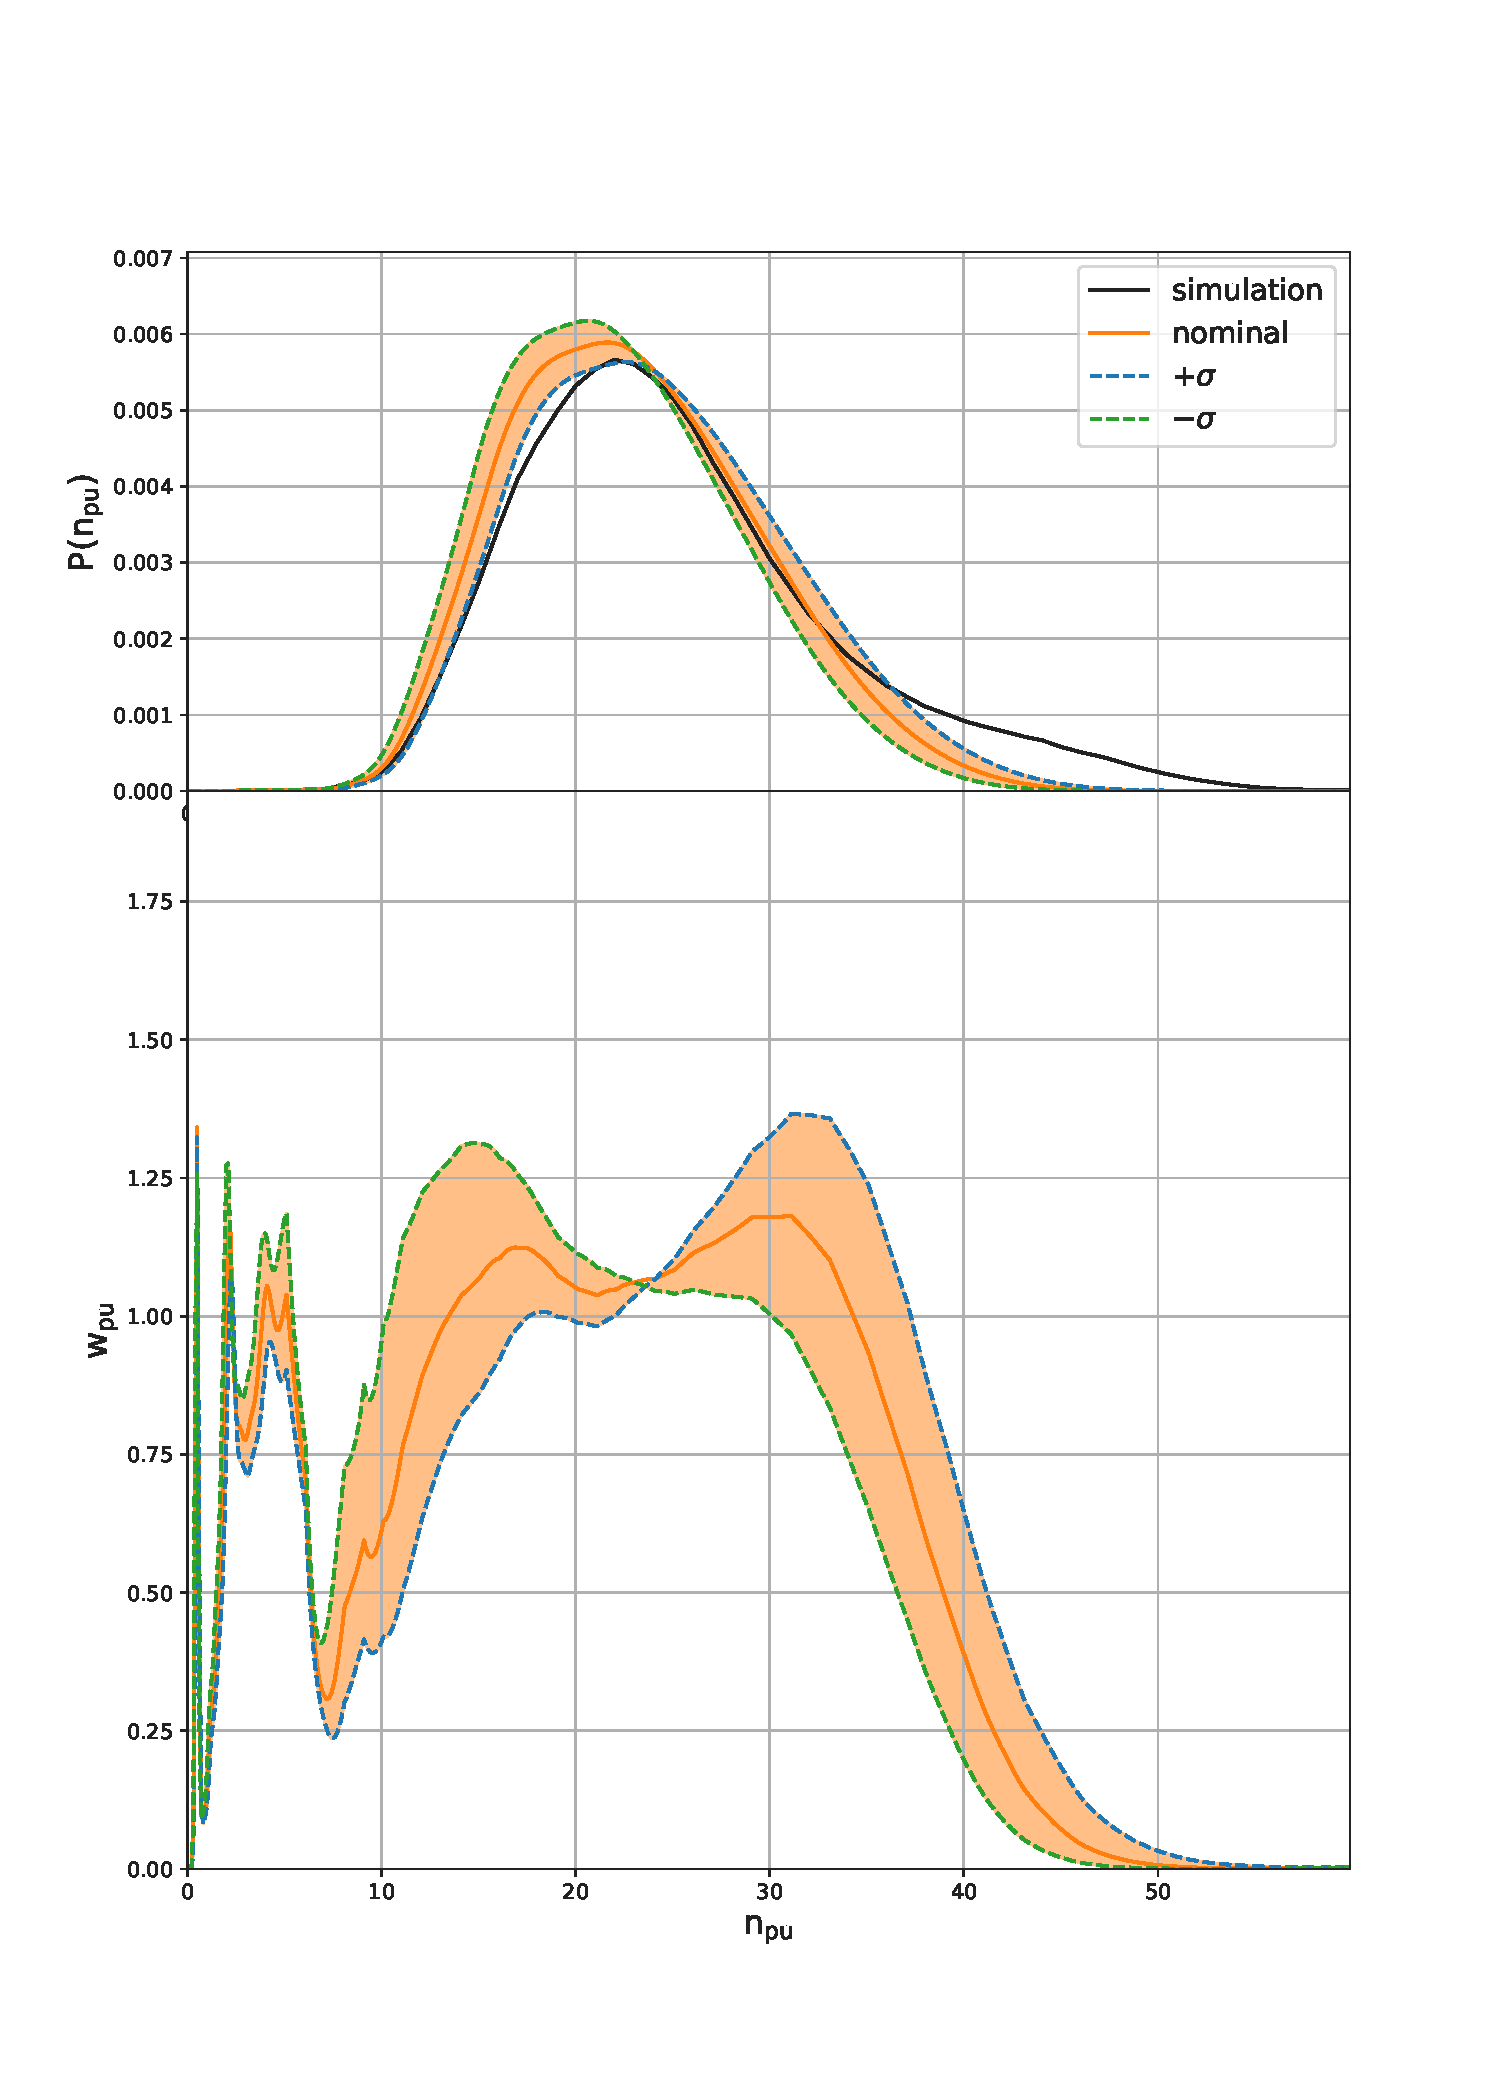
\includegraphics[width=\textwidth]{chapters/Analysis/sectionCalibration/figures/generator/pileup_systematics.pdf}
        \end{block}
        
        % add column
        \column{0.24\textwidth}
        \begin{block}{top \pt}
            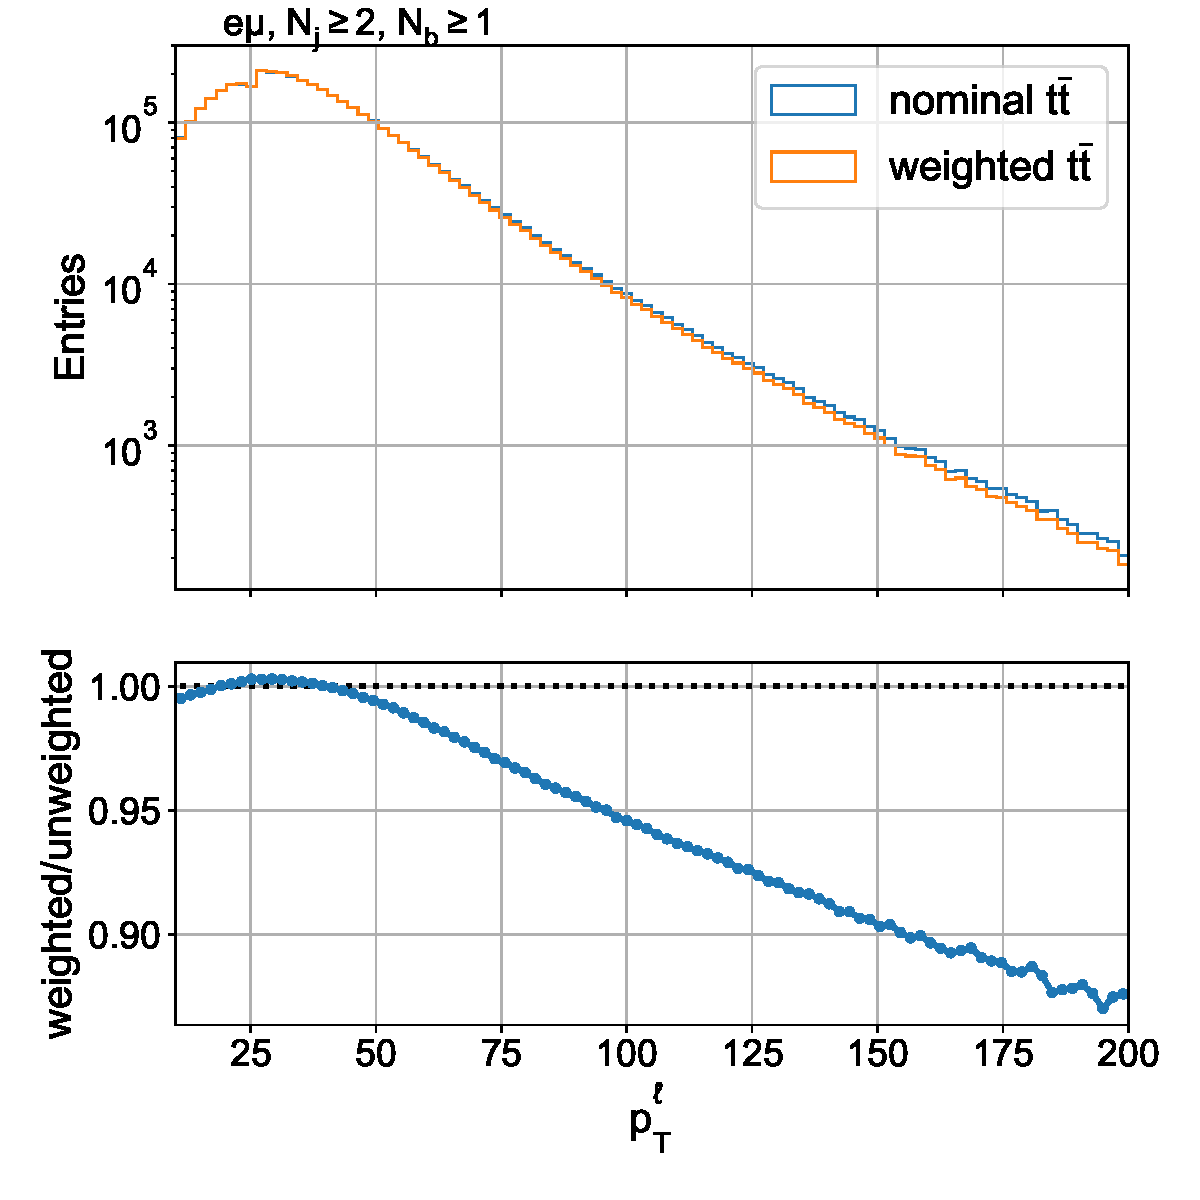
\includegraphics[width=\textwidth]{chapters/Analysis/sectionCalibration/figures/generator/top_pt_weight.pdf}
        \end{block}
        % add column
        \column{0.24\textwidth}
        \begin{block}{\PZ \pt}
            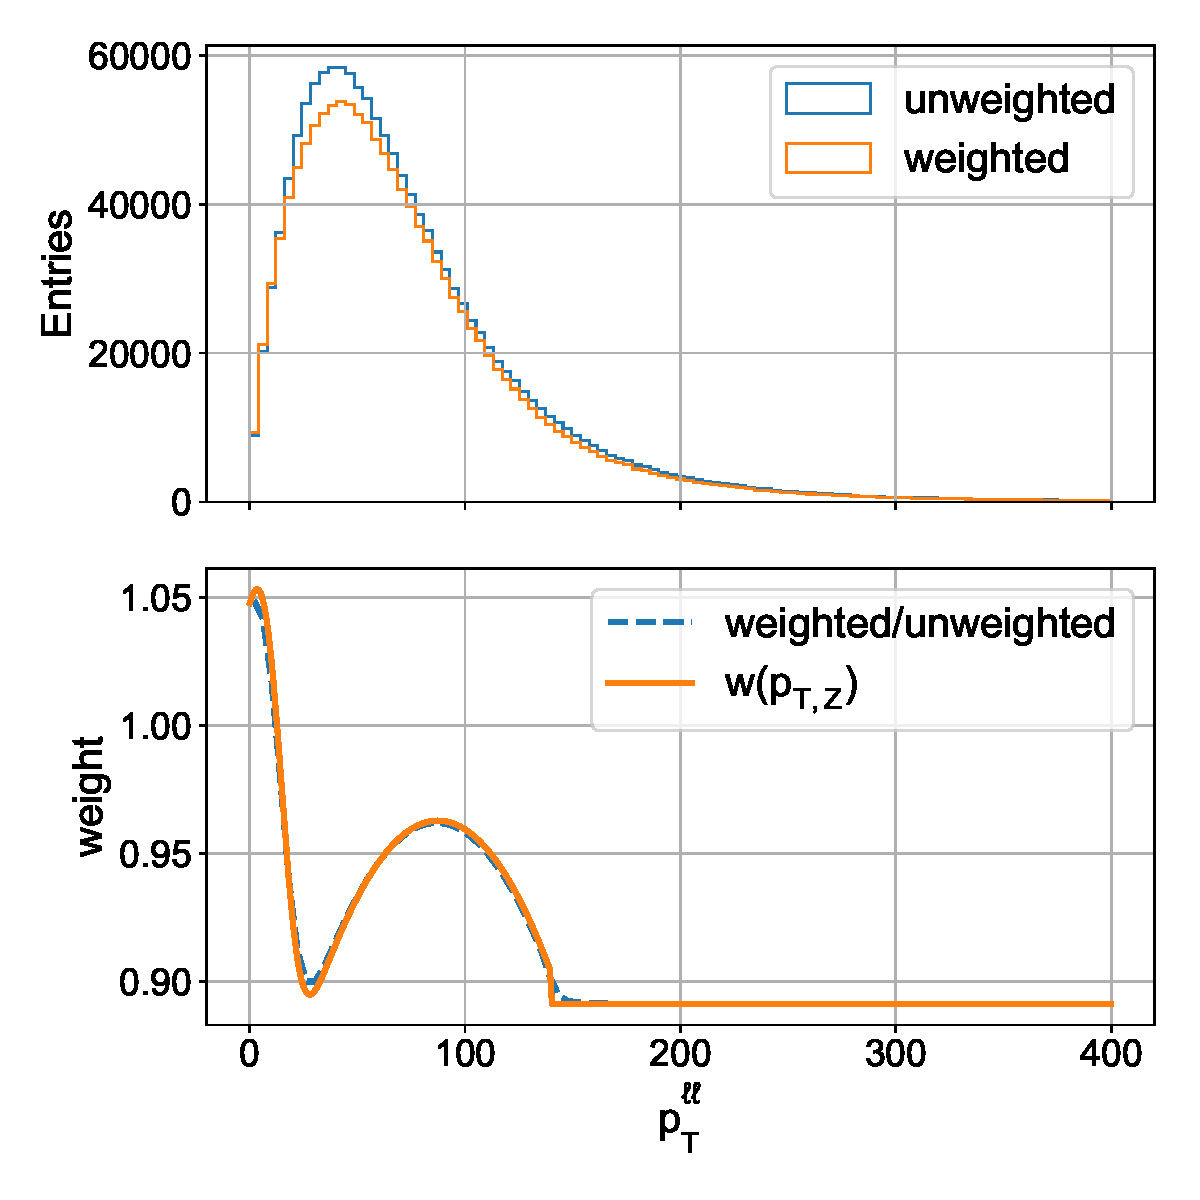
\includegraphics[width=\textwidth]{chapters/Analysis/sectionCalibration/figures/generator/z_pt_weighting.pdf}
        \end{block}
         % add column
        \column{0.24\textwidth}
        \begin{block}{\WW \pt}
            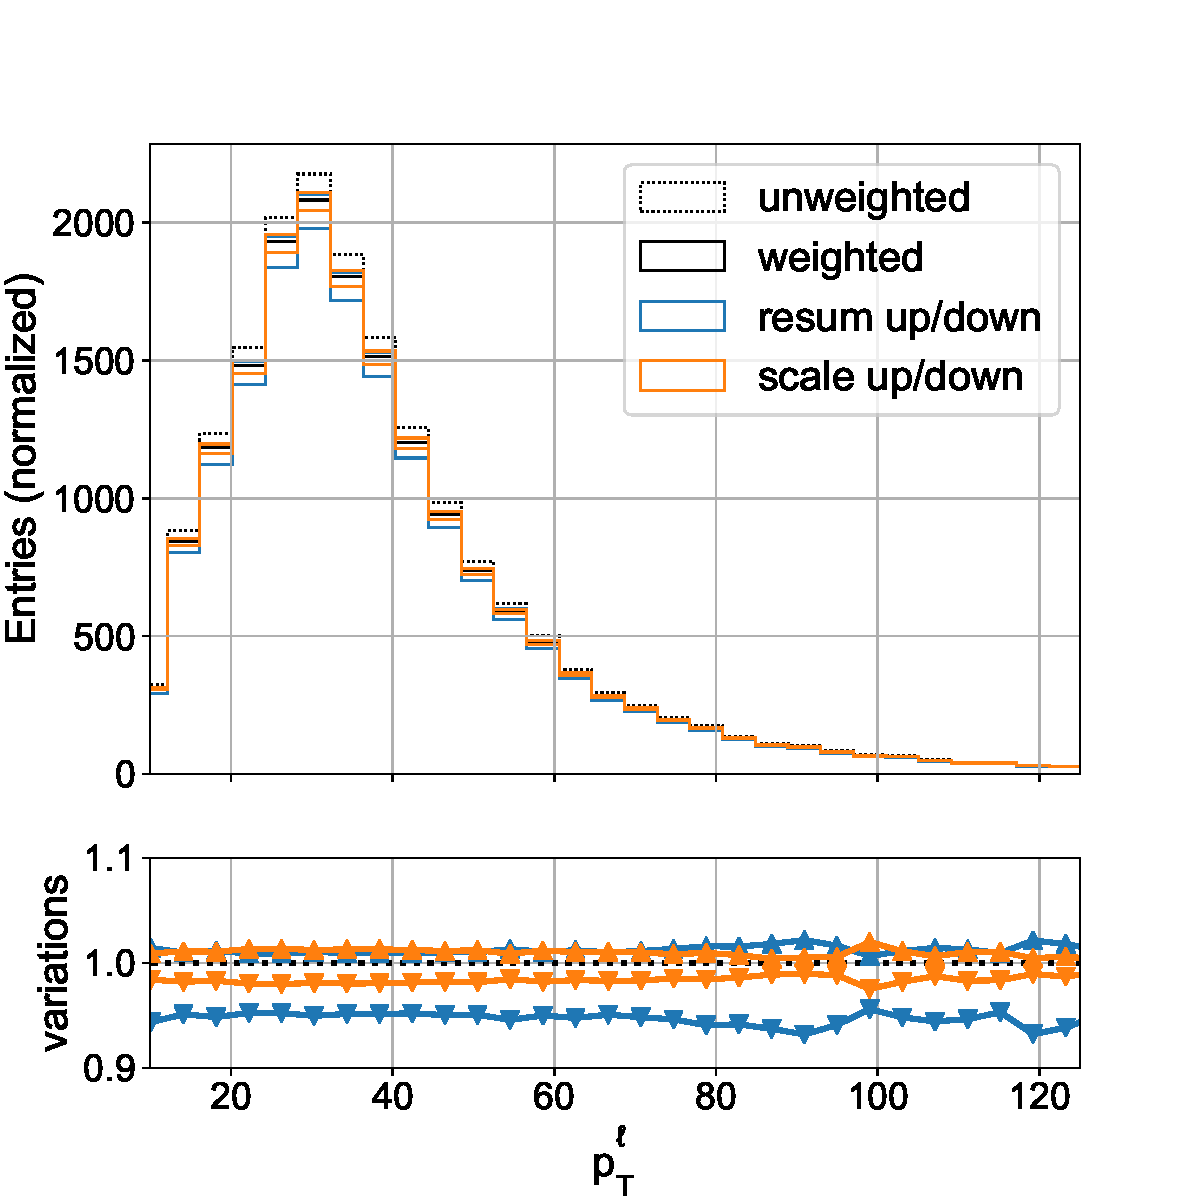
\includegraphics[width=\textwidth]{chapters/Analysis/sectionCalibration/figures/generator/ww_pt_lepton_pt.pdf}
        \end{block}
            
    \end{columns}
\end{frame}


% -------------
% new frame
% -------------
\begin{frame}{}
\smaller
    \begin{columns}
        \column{0.48\textwidth}
        \begin{exampleblock}{electron}
            \begin{itemize} 
            \smaller
                \item energy scale and energy resolution
                \item reconstruction efficiency
                \item isolation efficiency
            \end{itemize}
        \end{exampleblock}
        
        \column{0.48\textwidth}
        \begin{exampleblock}{muon}
            \begin{itemize} 
            \smaller
                \item energy scale
                \item identification efficiency
                \item isolation efficiency
            \end{itemize}
        \end{exampleblock}
    \end{columns}
        

    \begin{exampleblock}{hadronic tau}
        \begin{itemize} 
        \smaller
            \item energy scale depending on reconstruction modes, derived by fitting $m_\PGth$ or $m_\ell\PGth$. We used the calibration from $m_\ell\PGth$ fit. 
            $$\PGt \to \mathrm{h}^{\pm}:0.995(5), \quad \PGt \to \mathrm{h}^{\pm}\PGpz:1.011(3), \quad \PGt \to \mathrm{h}^{\pm}\mathrm{h}^{\mp}\mathrm{h}^{\pm}\PGpz:1.006(3)$$
                

            \item identification efficiency, derived from $\PZ \to \PGtl \PGth$ and $\ttbar \to \ell \PGth$ region. We use the calibration from $\PZ \to \PGtl \PGth$ region.
            $$\text{0.95(5) --- Tight, 0.92(5) --- VTight working point}$$
            
            \item $j\to\PGth$. customized measured of $j\to\PGth$ scale factors with \pt and jet flavor depedence.
        \end{itemize}
    \end{exampleblock}
    
    \begin{columns}
        \column{0.48\textwidth}
        \begin{exampleblock}{jet}
            \begin{itemize} 
            \smaller
                \item energy scale and energy resolution
            \end{itemize}
        \end{exampleblock}
        \column{0.48\textwidth}

        
        \begin{exampleblock}{b tag}
            \begin{itemize} 
            \smaller
                \item tag efficiency 
                \item mistag probability
                \item promote/demote approach
            \end{itemize}
        \end{exampleblock}
    \end{columns}
\end{frame}


% -------------
% new frame
% -------------
\begin{frame}{}
\smaller
    \begin{columns}
    \column{.49\textwidth}
     \begin{block}{muon trigger}
        \centering
        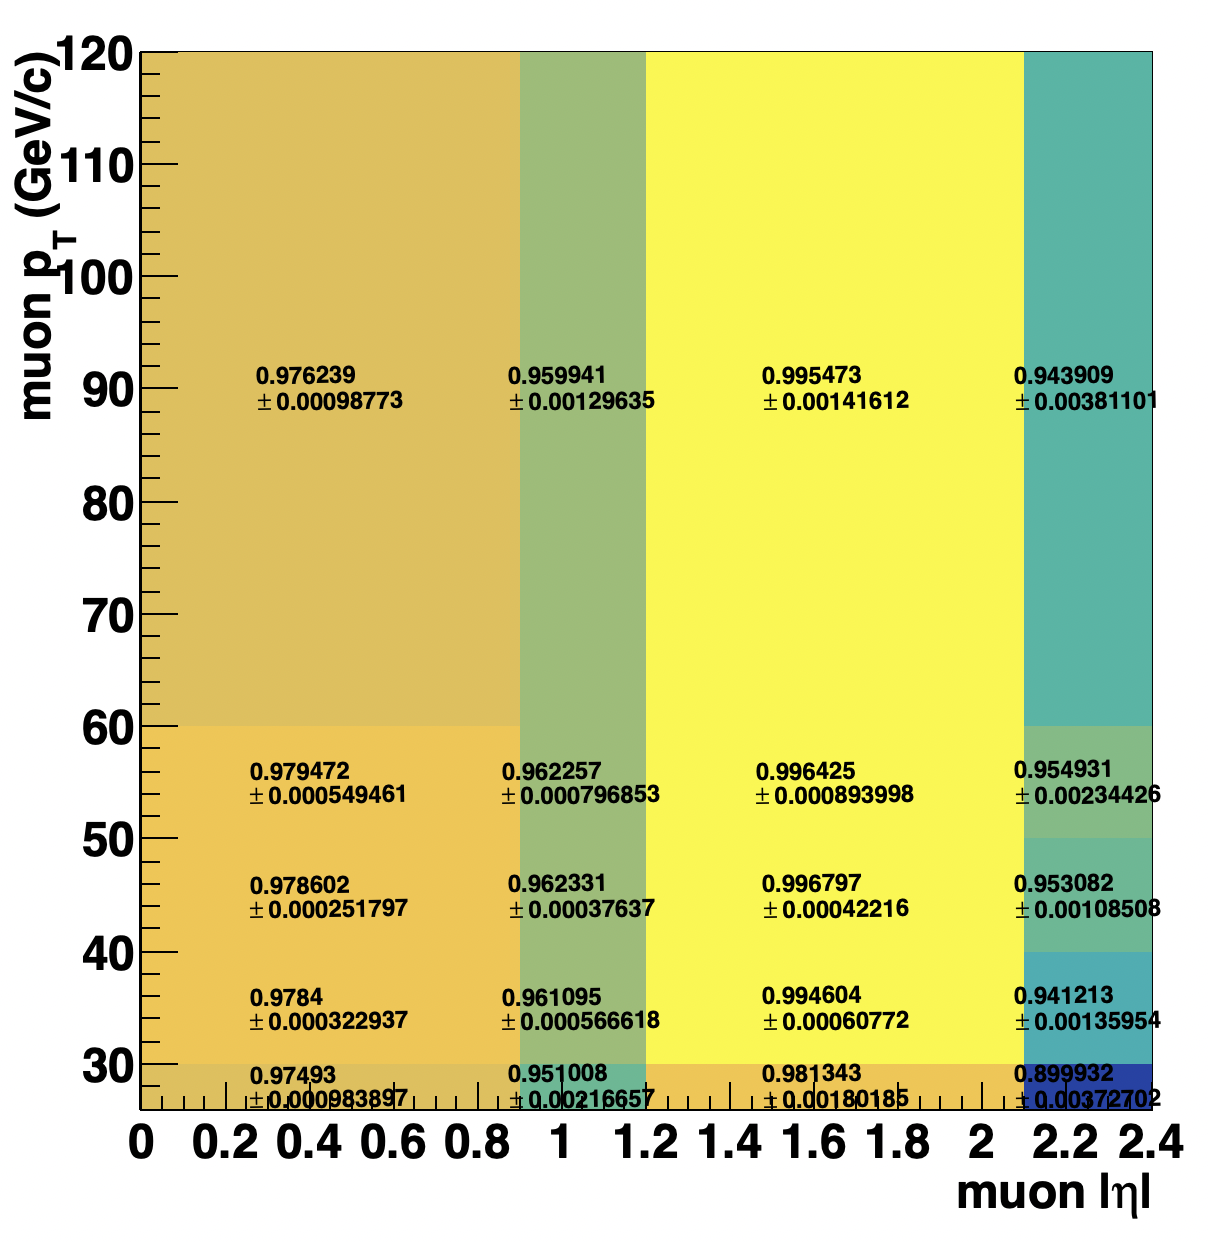
\includegraphics[width=0.45\textwidth]{chapters/Analysis/sectionCalibration/figures/trigger/muTrSF_BCDEF.png}
        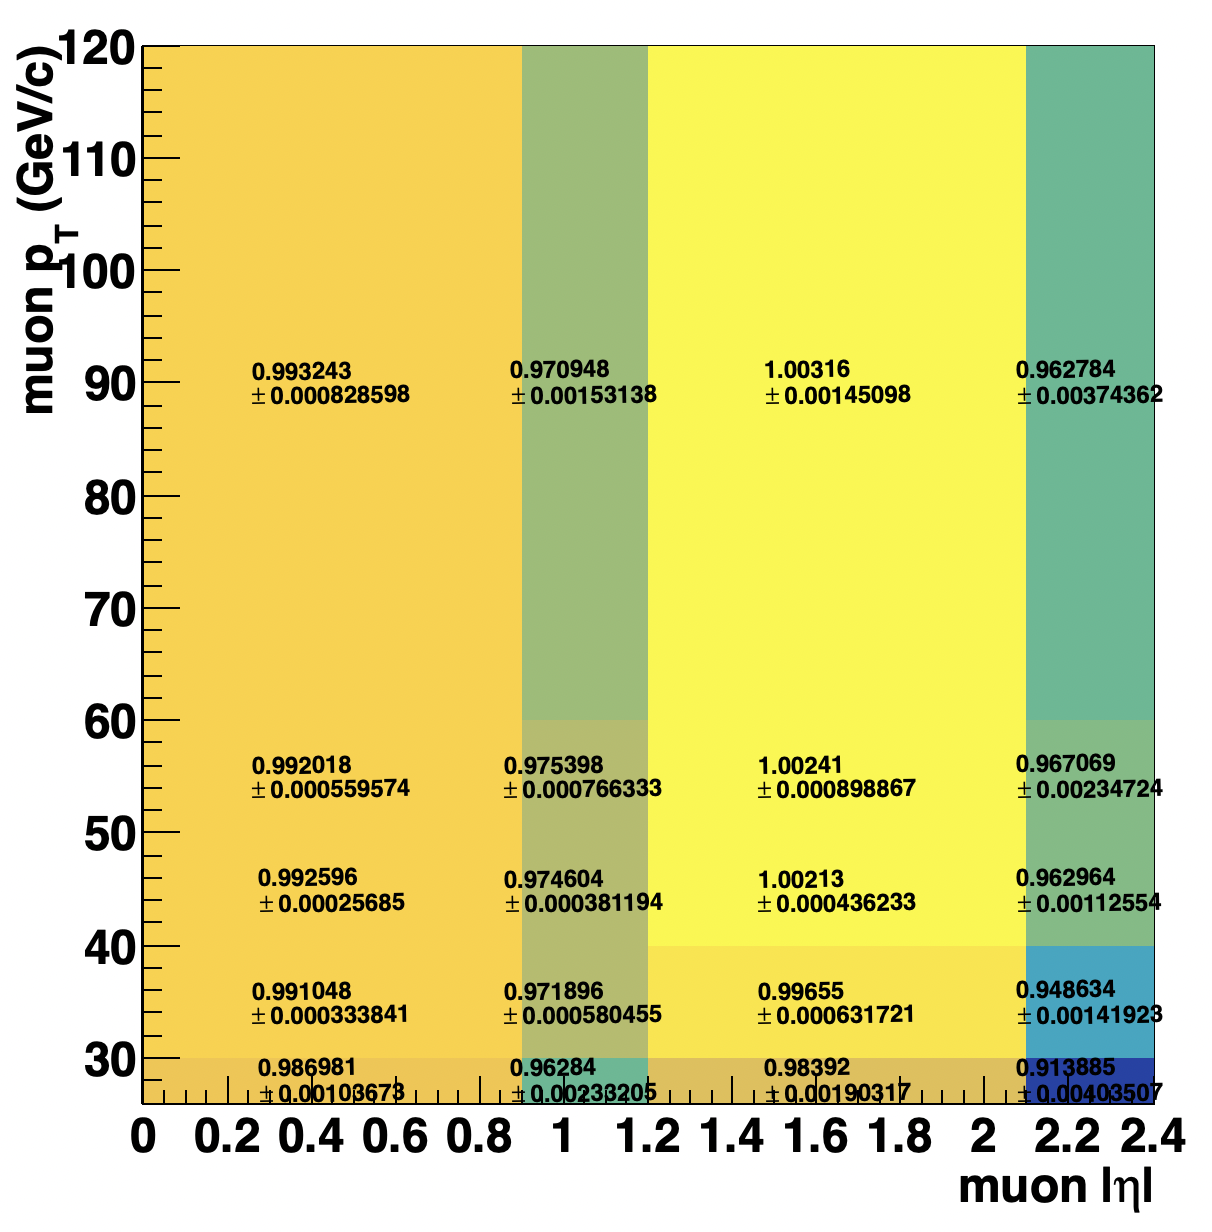
\includegraphics[width=0.45\textwidth]{chapters/Analysis/sectionCalibration/figures/trigger/muTrSF_GH.png}
    \end{block} 
    
    \column{.49\textwidth}
     \begin{block}{electron trigger}
        \centering
        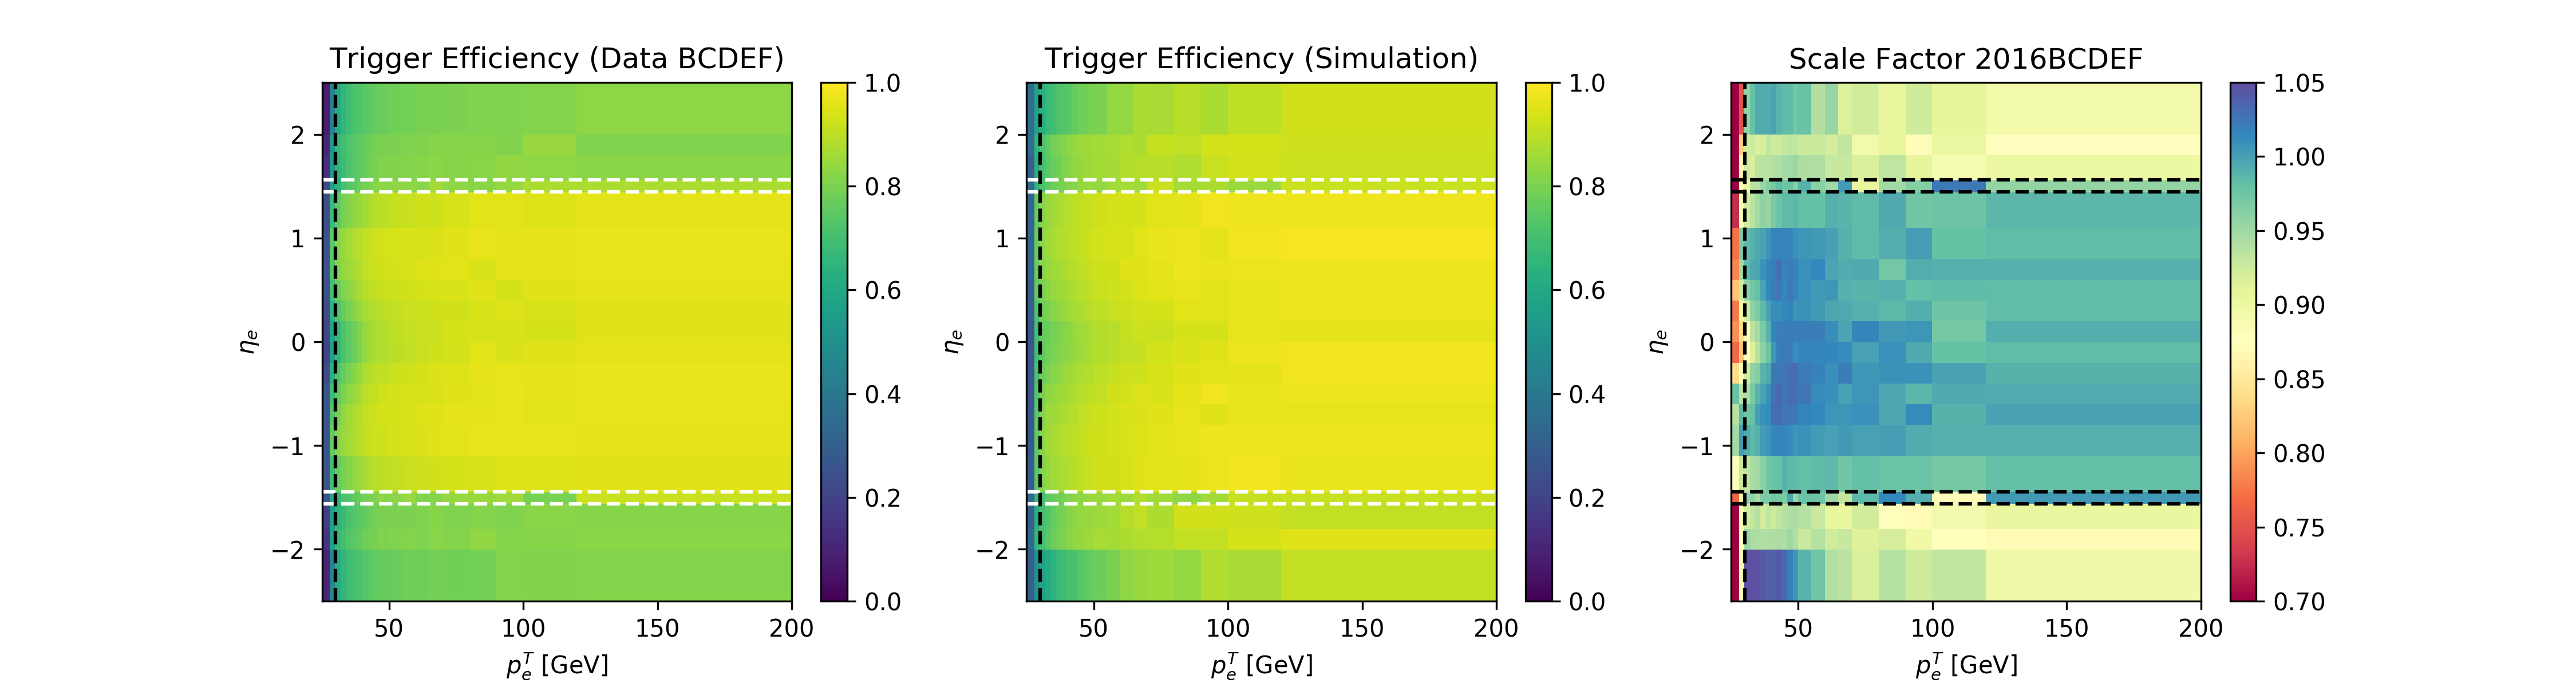
\includegraphics[width=0.45\textwidth, trim=24cm 0 3.7cm 0, clip]{chapters/Analysis/sectionCalibration/figures/eTrigger/eff2d_BCDEF.png}
        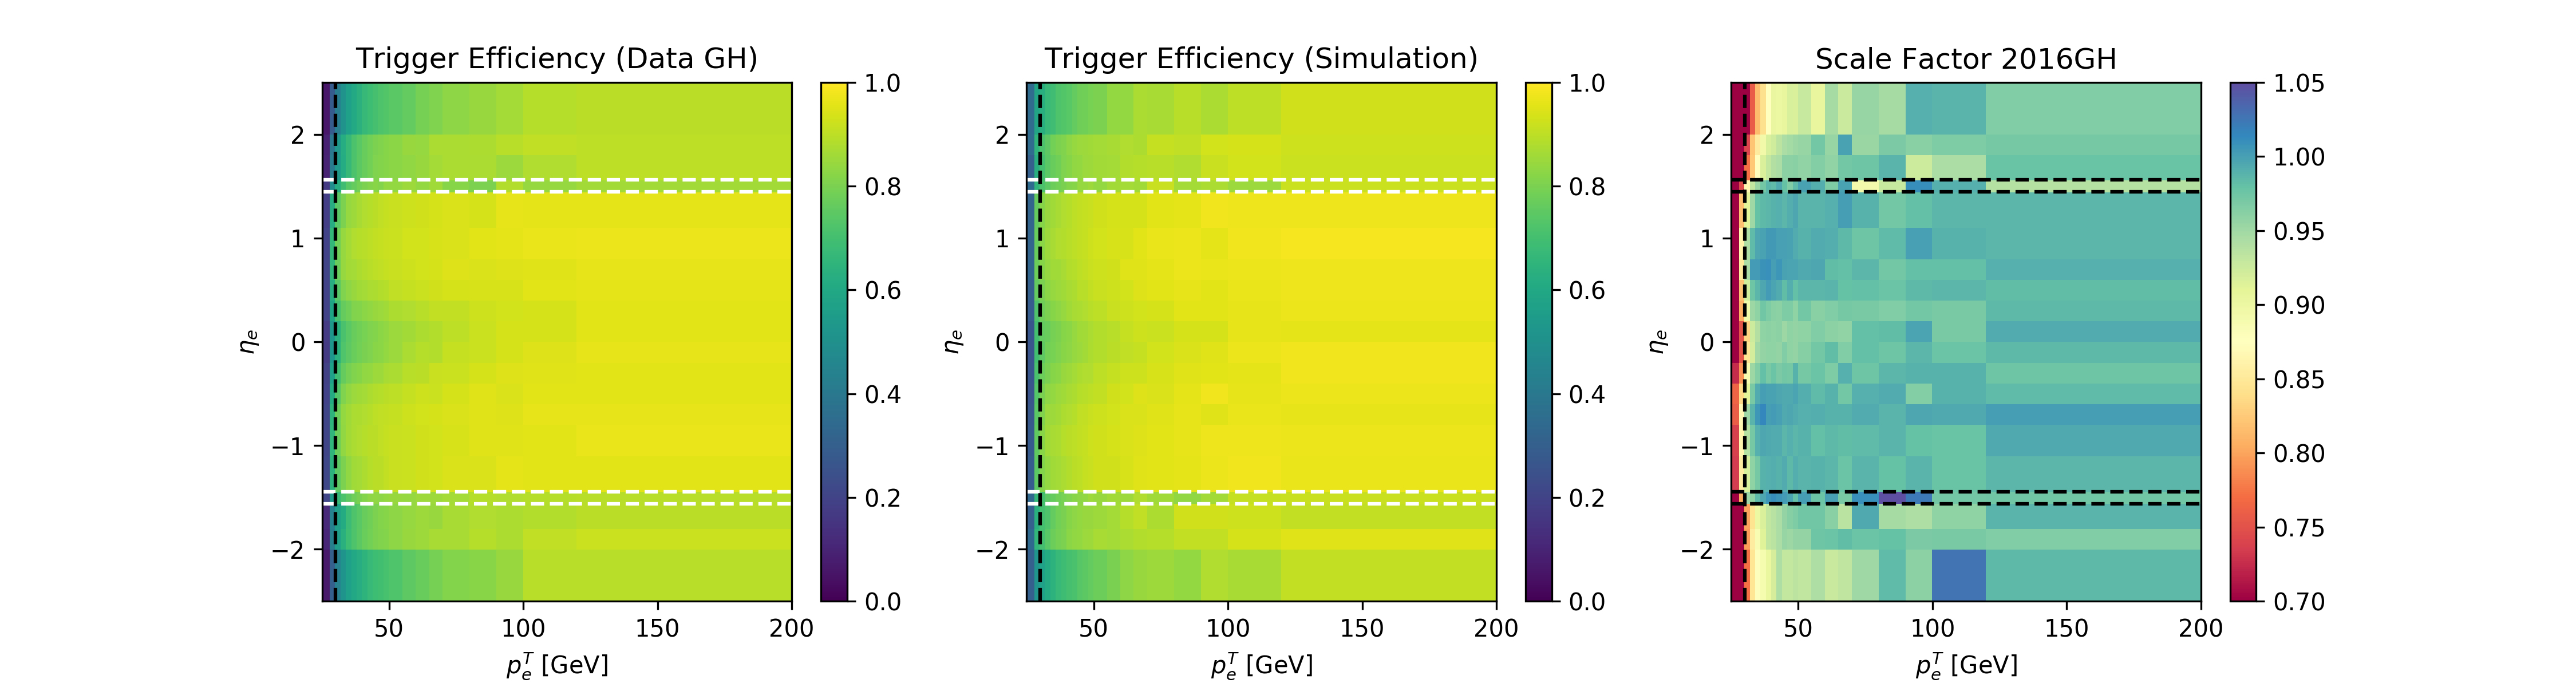
\includegraphics[width=0.45\textwidth, trim=24cm 0 3.7cm 0, clip]{chapters/Analysis/sectionCalibration/figures/eTrigger/eff2d_GH.png}
    \end{block}
    \end{columns}
    
    \begin{block}{electron prefiring correction}
        \begin{columns}
            \column{0.6\textwidth}
            \begin{itemize} 
                \smaller
                \item due to timing issue, L1T signal in higher eta could be treated as from previous bunching crossing by mistake.
                \item the wrong brunching crossing fails the HLT due to absence of the triggering objects, resulting data loss.
                \item this is not simulated. 
                \item corrected by a scale factor calculated from prefirable jets and photons $$ SF = \prod_{i=\PGg,jet}\bigg(1-\epsilon_i(\pt, \eta) \bigg) $$
                \item scale down the events by ~1\%.
            \end{itemize}
            
            \column{0.35\textwidth}
            % 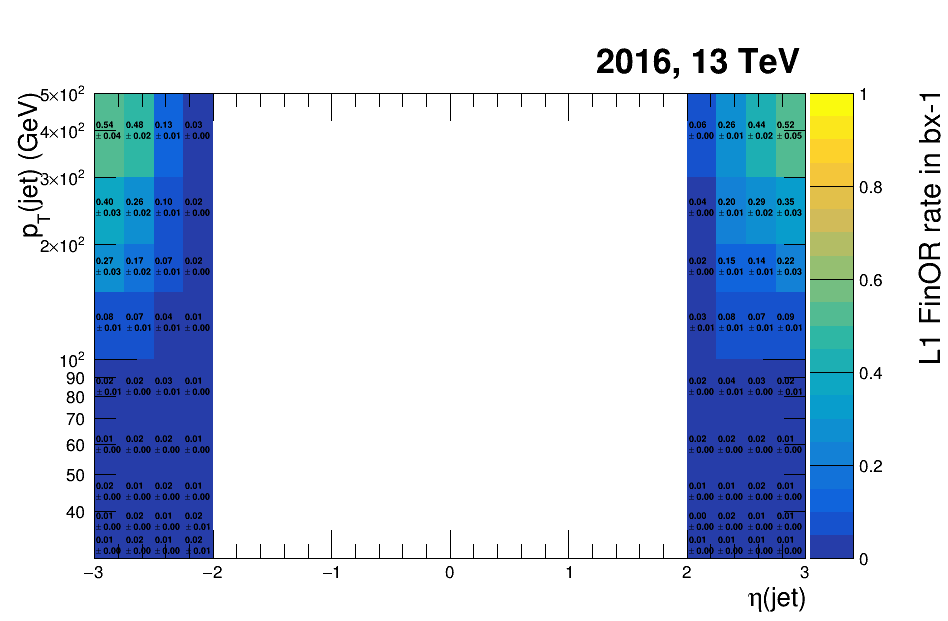
\includegraphics[width=\textwidth]{chapters/Analysis/sectionCalibration/figures/prefiring/L1prefiring_jetpt_2016BtoH.png}
            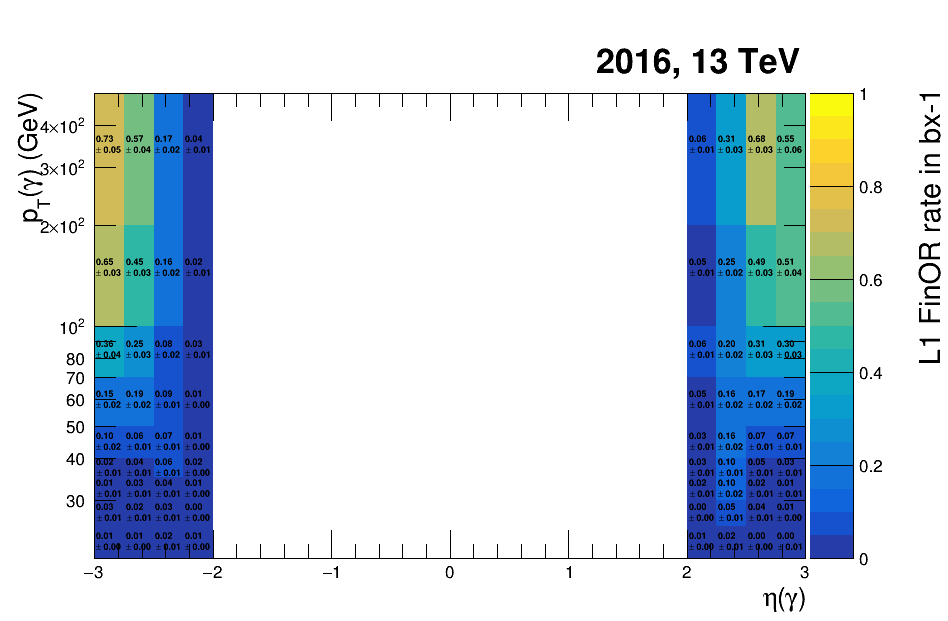
\includegraphics[width=\textwidth]{chapters/Analysis/sectionCalibration/figures/prefiring/L1prefiring_photonpt_2016BtoH.png}
            
        \end{columns}
    \end{block}

\end{frame}

% -------------
% new frame
% -------------
\begin{frame}{}
\smaller
    \begin{columns}
    \smaller 
        \column{0.6\textwidth}
        \begin{itemize} 
            \item measured with tag and prob approach.
            \begin{itemize} 
            \smaller \smaller
                \item tagged electron: $\pt > 30\GeV$ , matched with \texttt{HLT\_Ele27\_WPTight\_Gsf}
                \item two opposite electrons (at least one tagged)
                \item $60<m_{\cee}<120\GeV$
                \item dominated by \zjets.
                \item for each tagged electron, the other electron become prob for measurement.
            \end{itemize}
            \item trigger efficiency is defined as 
            $$ \epsilon (\pt, \eta) = \frac{ N_{\rm passing} (\pt, \eta) } {  N_{\rm total} (\pt, \eta) } $$
            the ratio of $\epsilon (\pt, \eta)$ between data and MC is 
            $$ SF (\pt, \eta) = \frac{\epsilon_{\rm{Data}} (\pt, \eta) }{\epsilon_{\rm{MC}} (\pt, \eta) }. $$
            
            \item split $SF (\pt, \eta)$ measurement into BCDEF and GH periods.
        \end{itemize}
        \column{0.4\textwidth}
        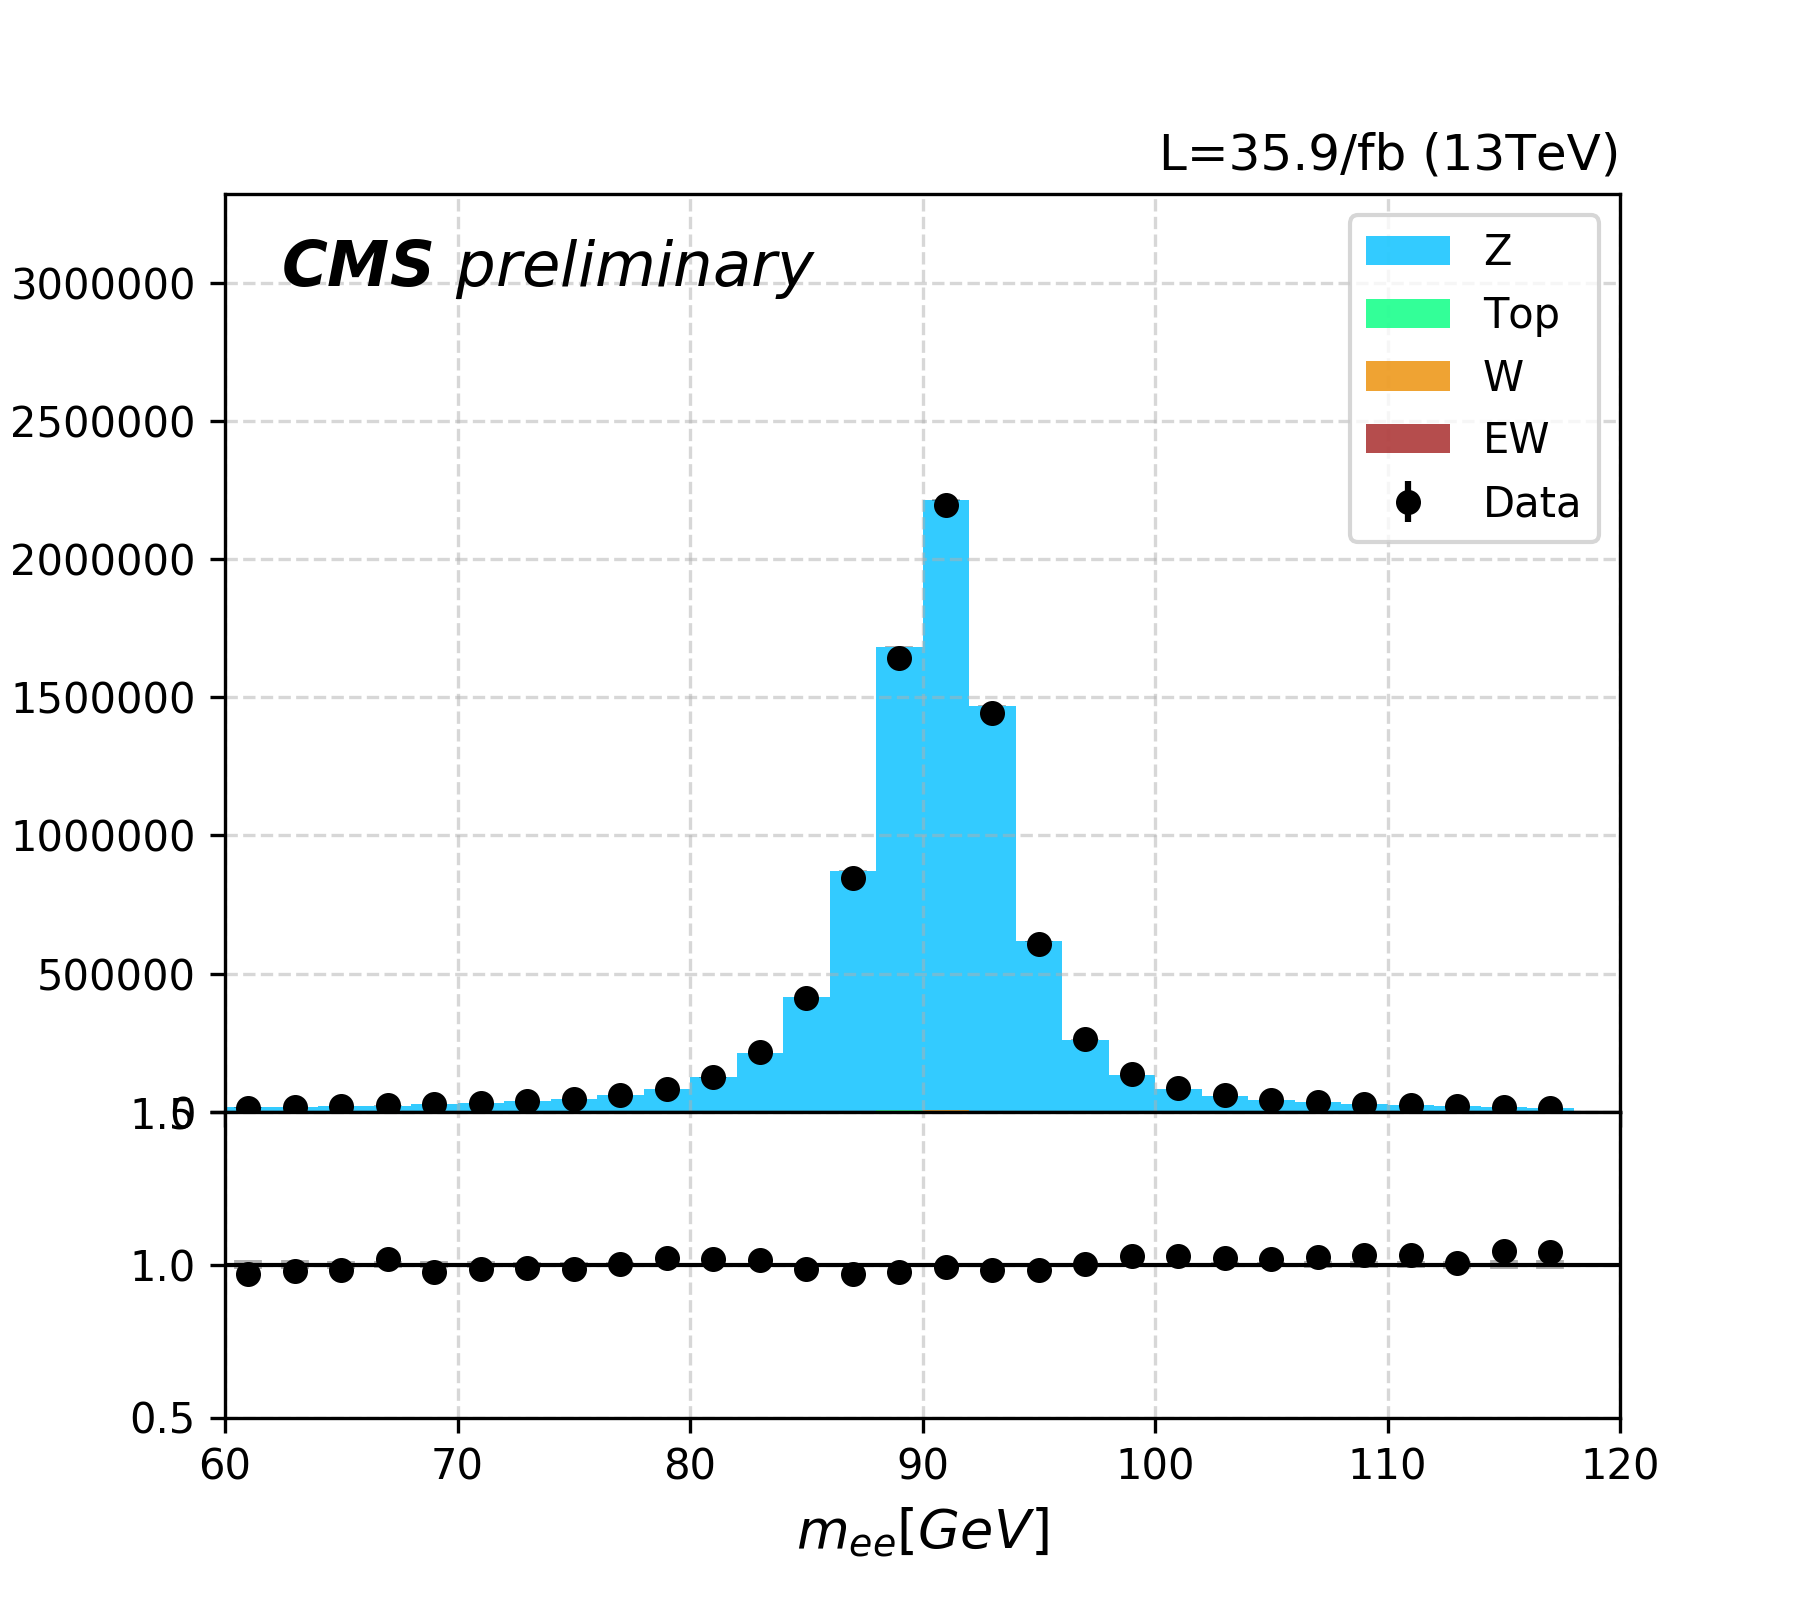
\includegraphics[width=\textwidth]{chapters/Analysis/sectionCalibration/figures/eTrigger/dileptonMass_tag30.png}
    \end{columns}
    
    \begin{center}
        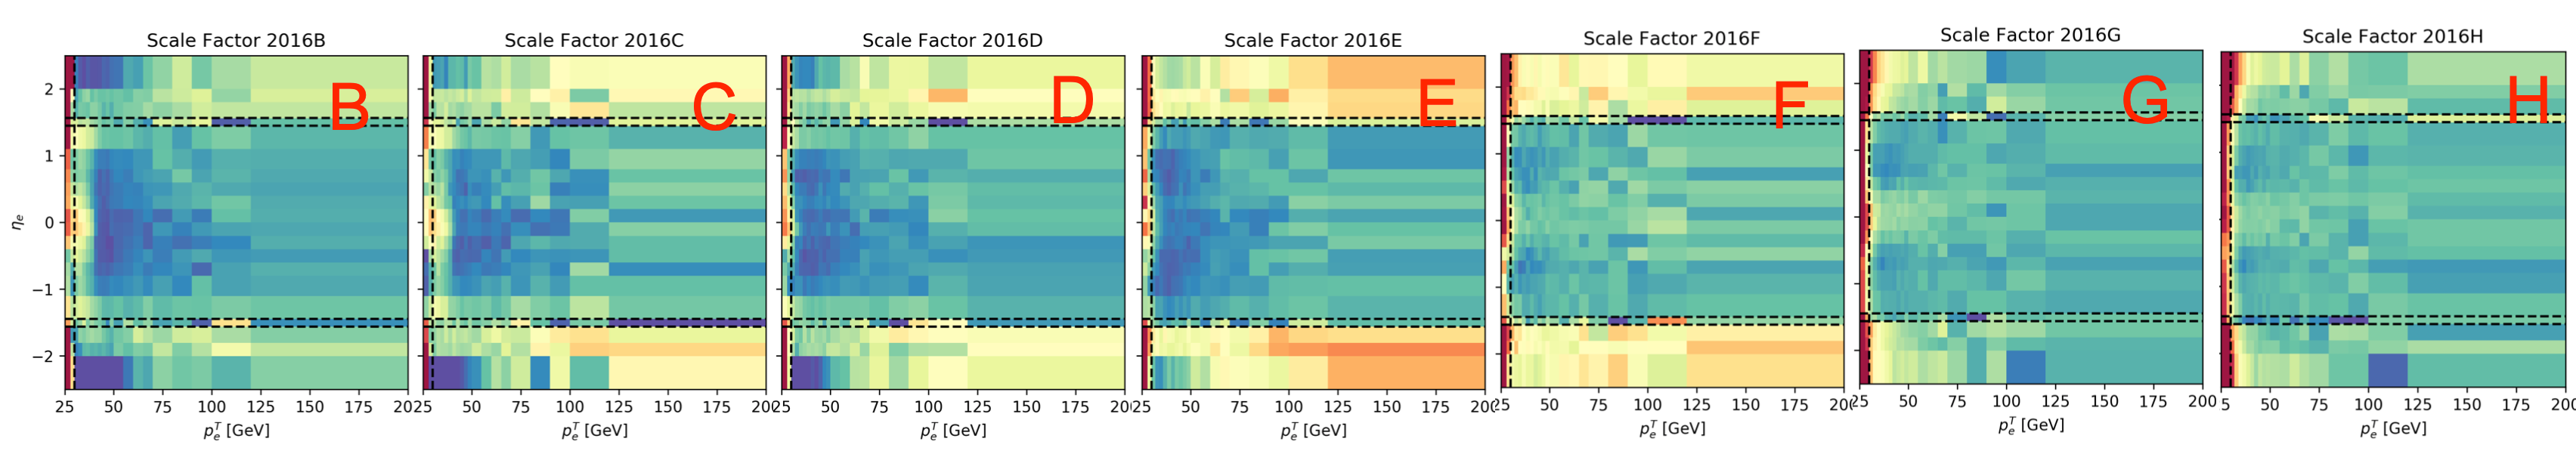
\includegraphics[width=\textwidth]{chapters/Analysis/sectionCalibration/figures/eTrigger/result_period.png}
    \end{center}
\end{frame}



% -------------
% new frame
% -------------
\begin{frame}{}
\smaller
    \begin{center}
        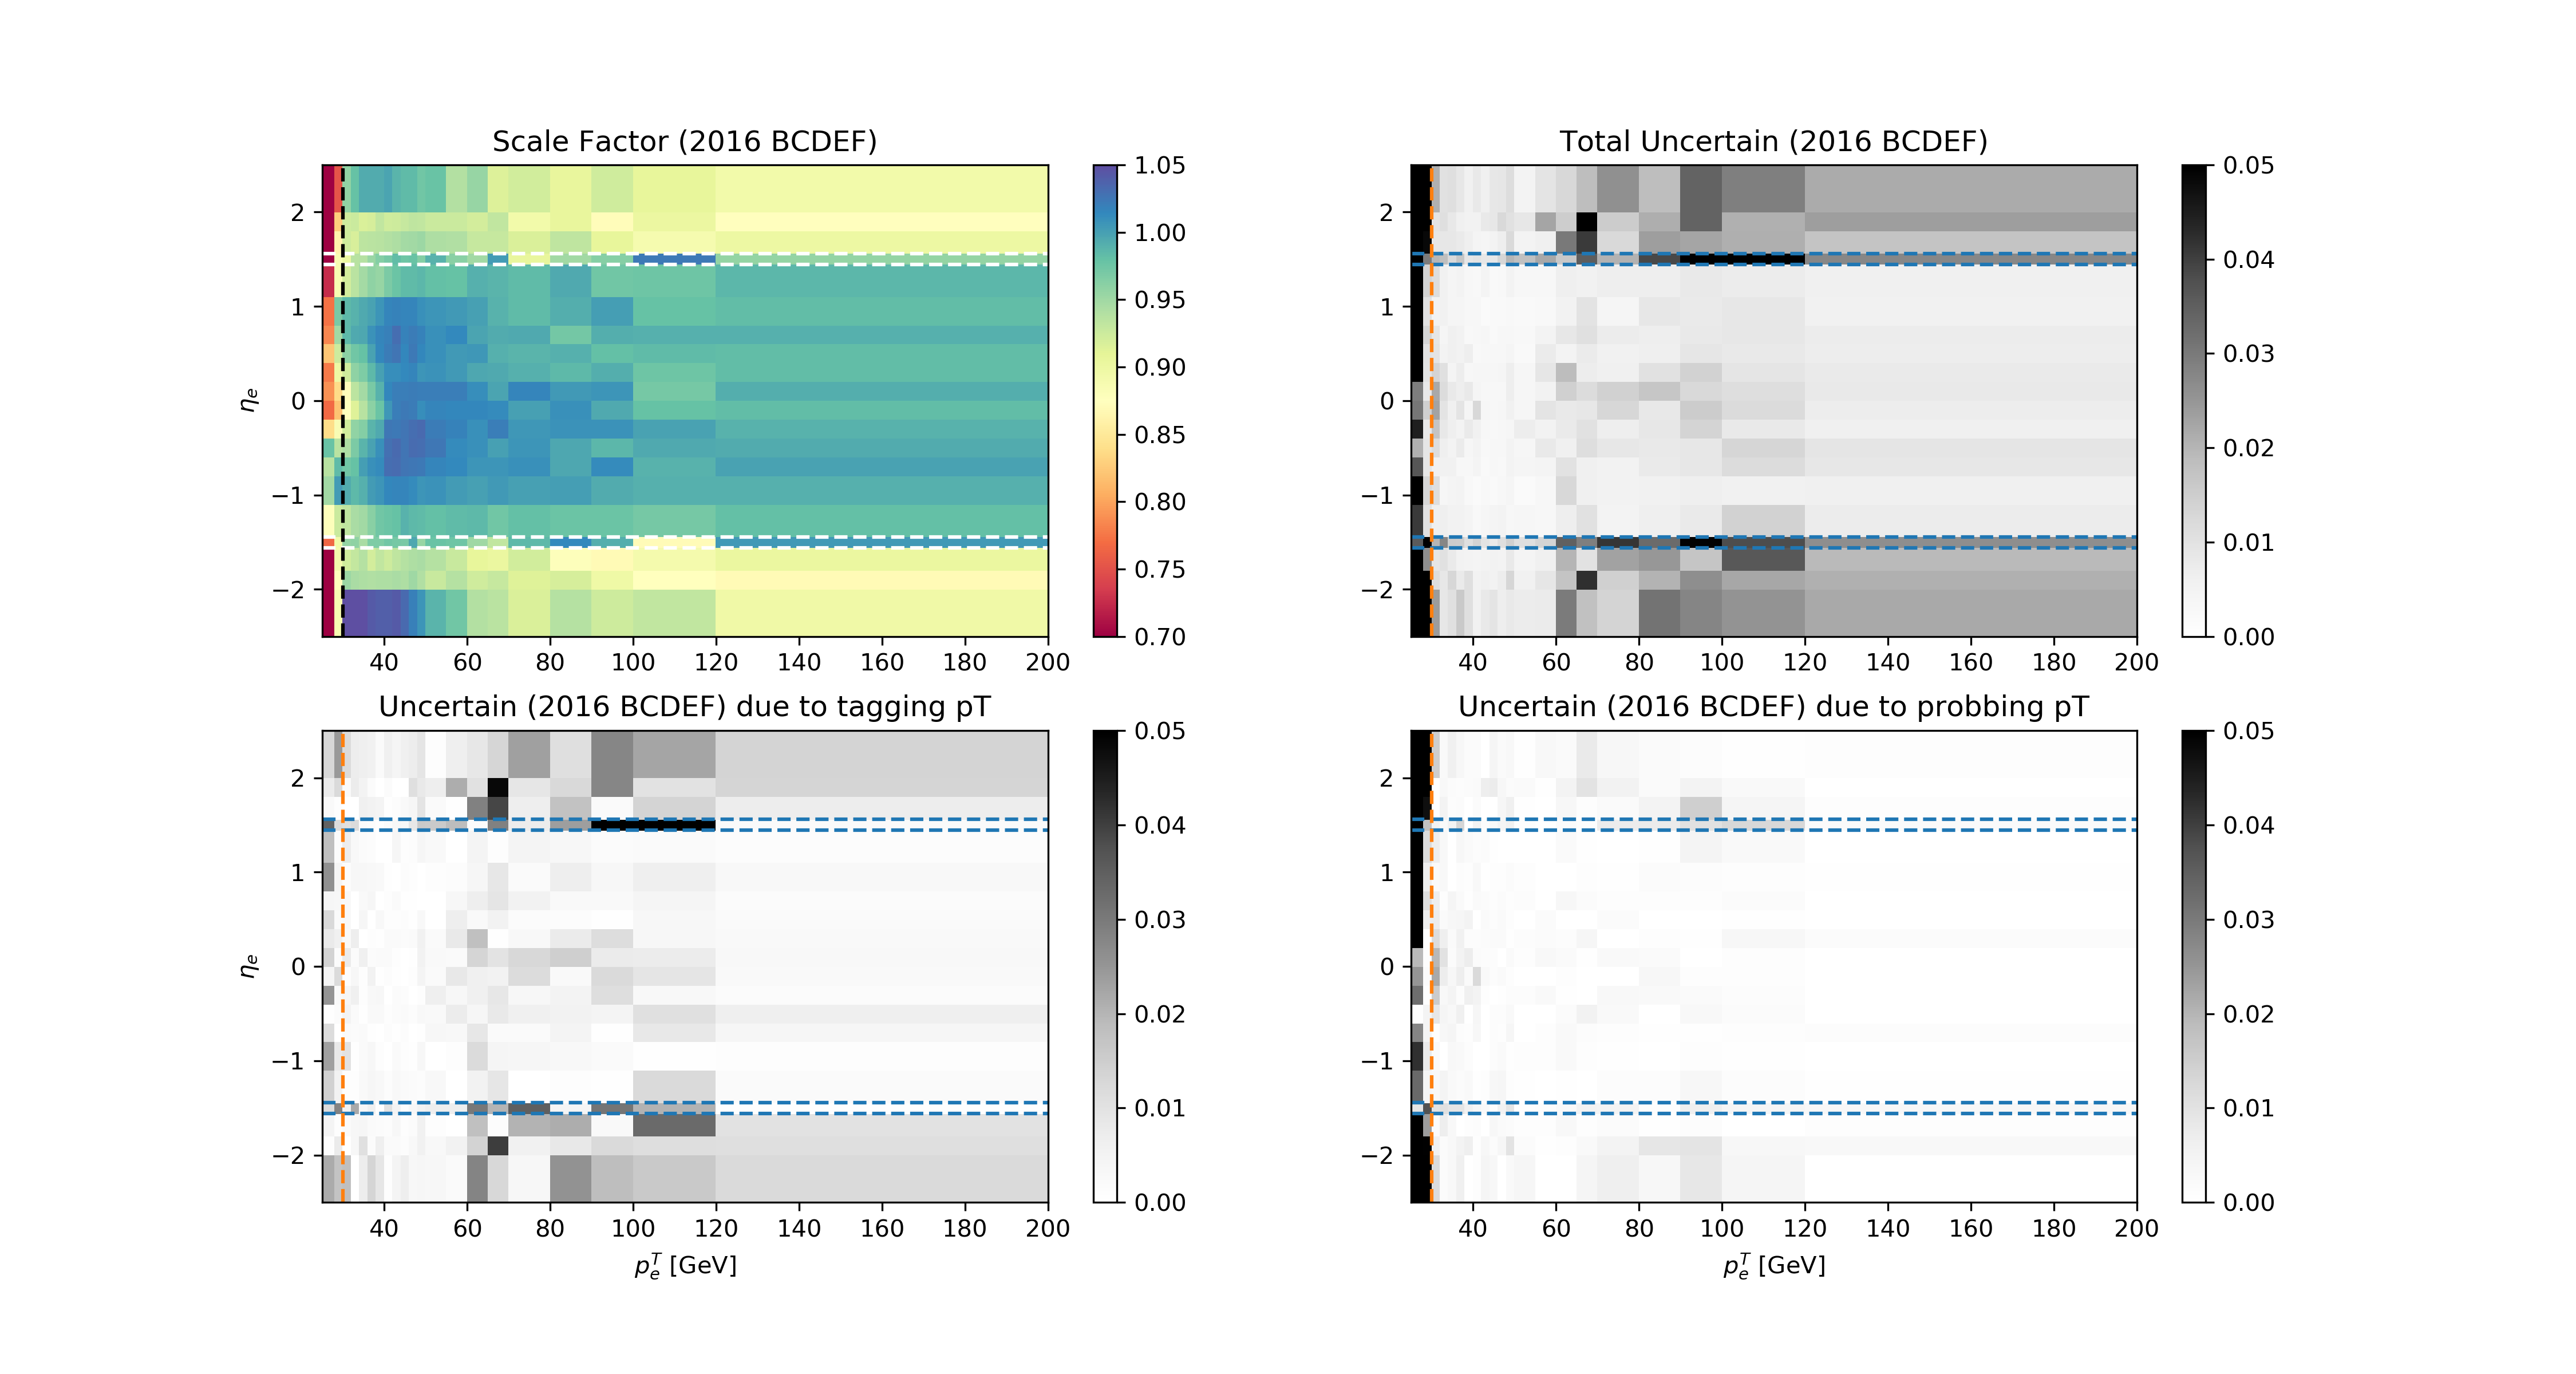
\includegraphics[width=0.49\textwidth,trim=3cm 0 3cm 0, clip]{chapters/Analysis/sectionCalibration/figures/eTrigger/result_BCDEF.png}
        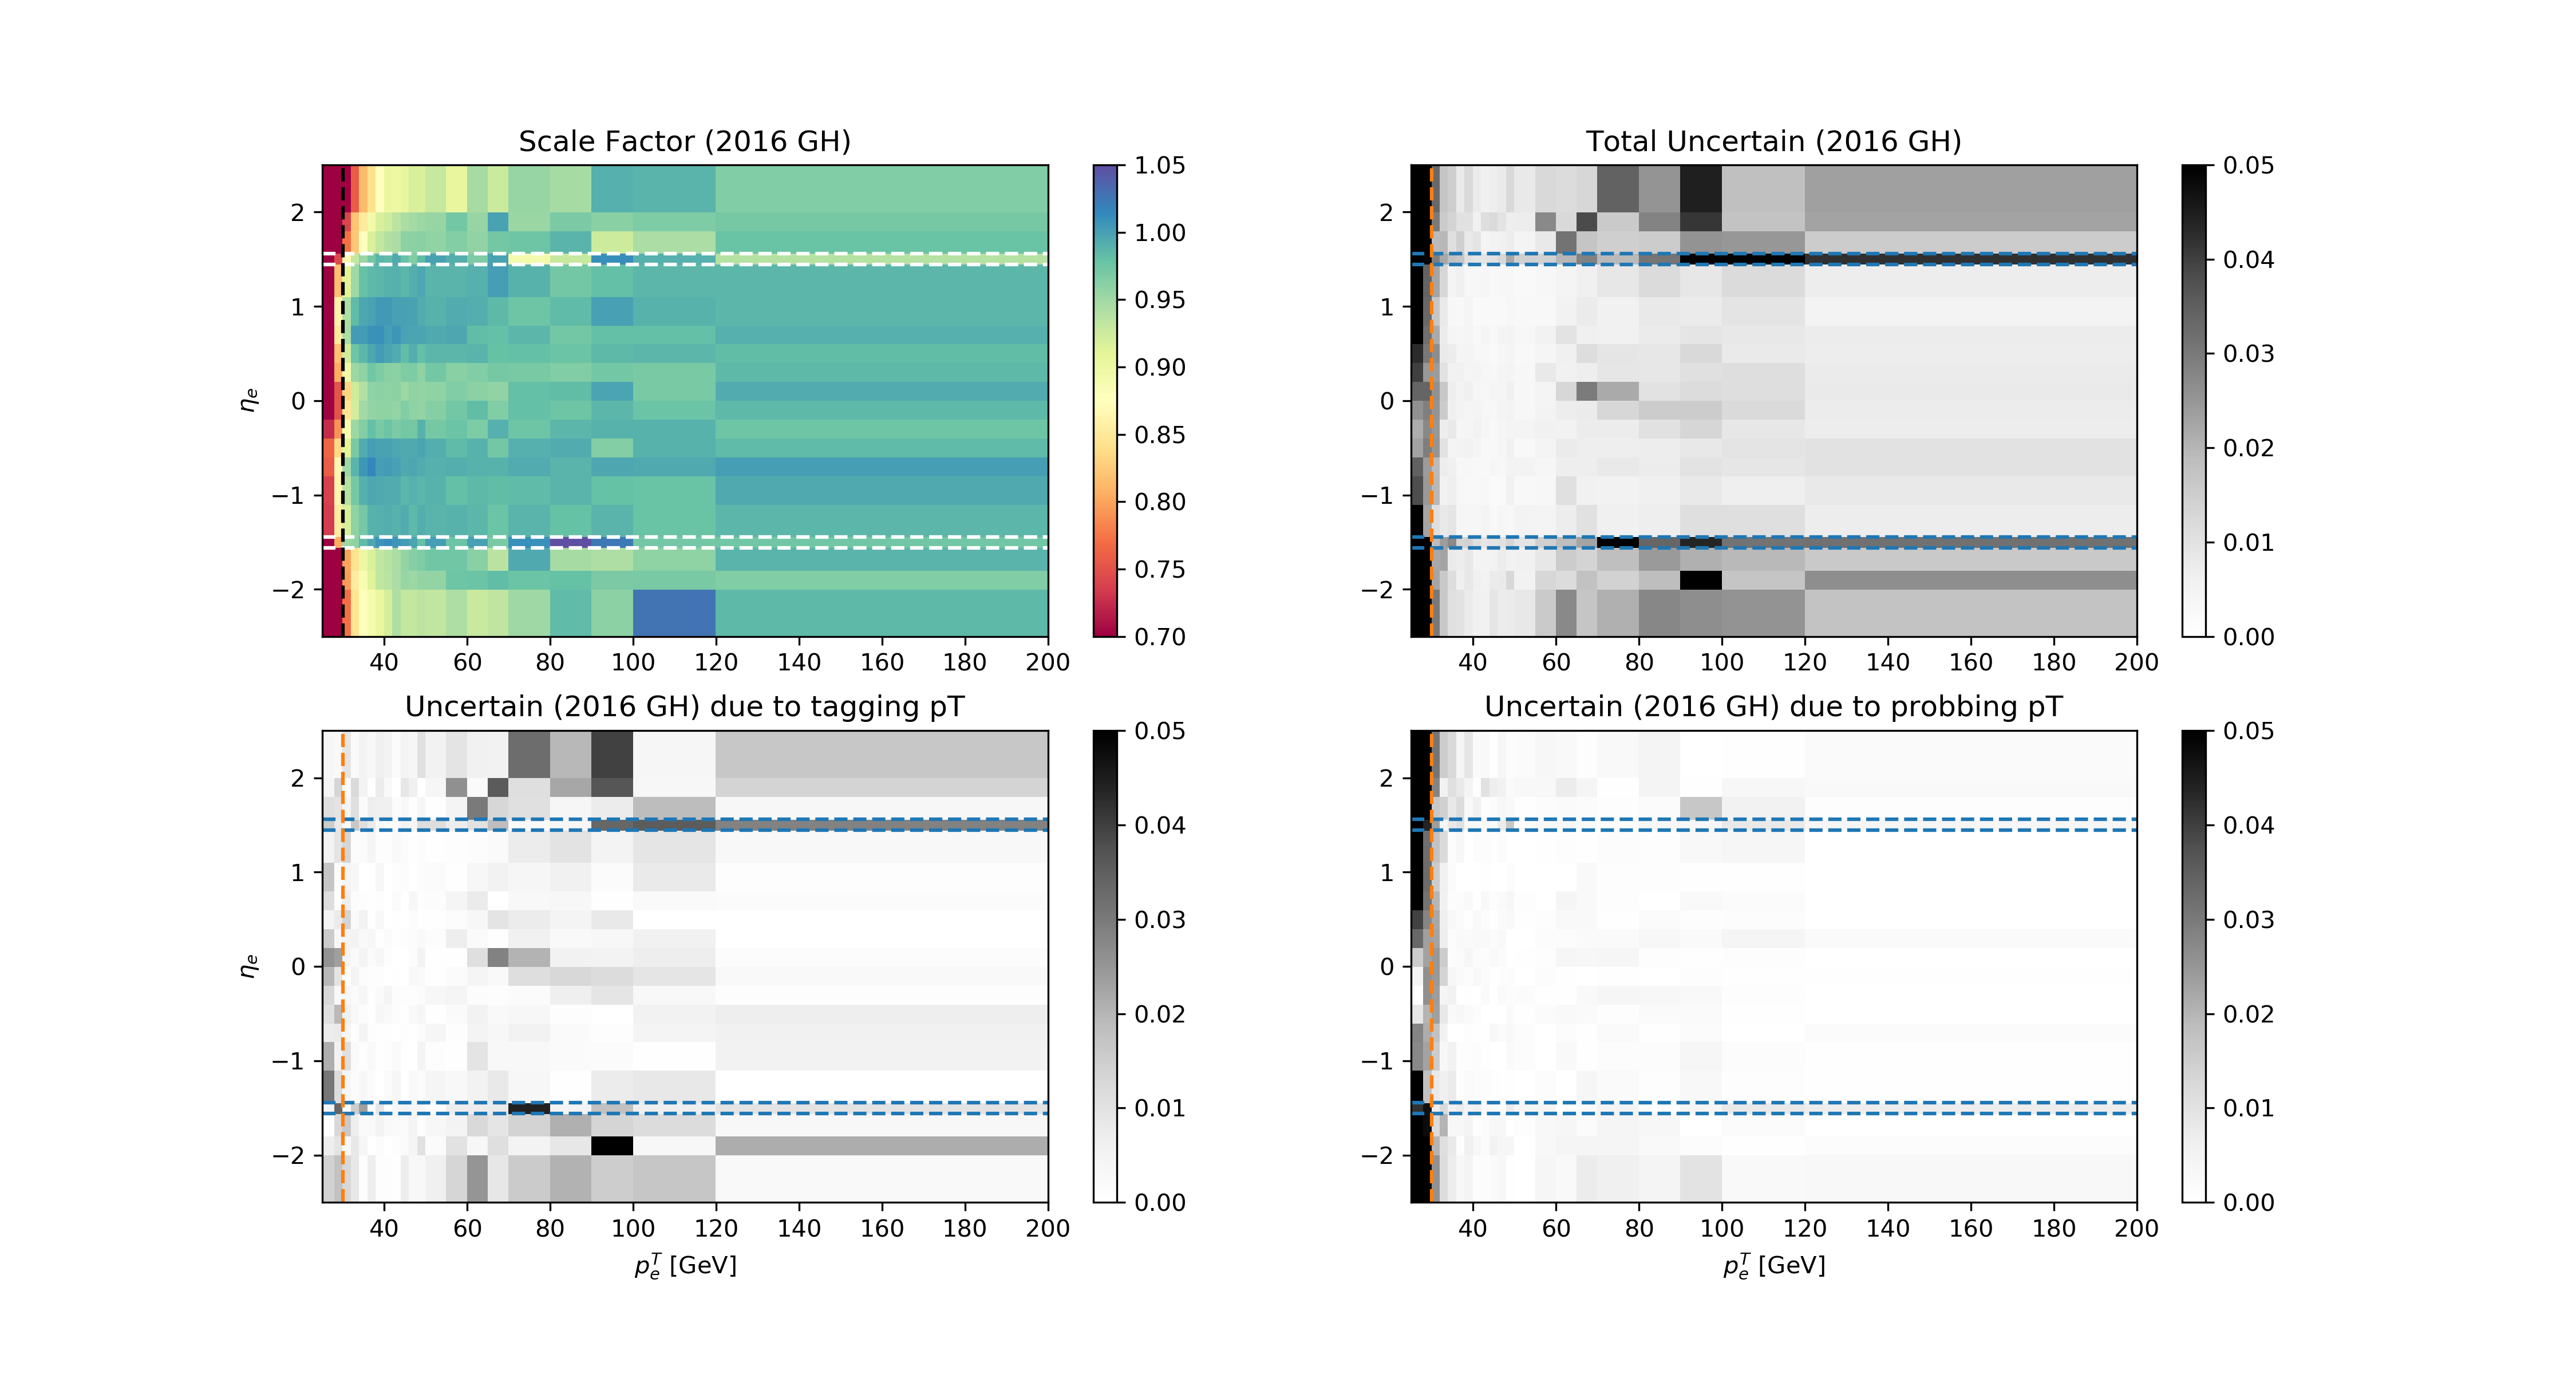
\includegraphics[width=0.49\textwidth,trim=3cm 0 3cm 0, clip]{chapters/Analysis/sectionCalibration/figures/eTrigger/result_GH.png}
    \end{center}
    
    \begin{itemize}
        \item the systematic uncertainty of the $SF (\pt, \eta)$ is estimated by ``two shifts"
        \begin{itemize}
        \smaller
            \item shift up the \pt threshold for tagging electron by 10\GeV to simulate a different trigger. This estimates the systematical effect that some L1 seed could have a threshold of 32\GeV.
            \item shift up and down the probing electron \pt by 0.5\GeV. This estimates the effect of the electron energy scale.
        \end{itemize}
    \end{itemize}
\end{frame}





% -------------
% new frame
% -------------
\begin{frame}{$j\to \PGth$ Reweighting}
\smaller
    \begin{itemize}
        \item Both signal and background MC contains $j\to \PGth$.
        \item correct these simulated events by $SF_{j\to \PGth}(\pt)$ 
        \item $SF_{j\to \PGth}(\pt)$ is measured in $j\to \PGth$ enriched regions
        \begin{itemize}
        \smaller
            \item $\cmm + \PGth$ and $\cmm + \PGth$ enriched with light jet faking \PGth.
            \item $\cem + \PGth$ enriched with b jet faking \PGth.
            \item from MC, the origins of \PGth are found by matching with gen-level particles.
        \end{itemize}
        \item both Tight and VTight tau identification working points are considered.
    \end{itemize}
\end{frame}


% -------------
% new frame
% -------------
\begin{frame}{}
\smaller
    \begin{center}
        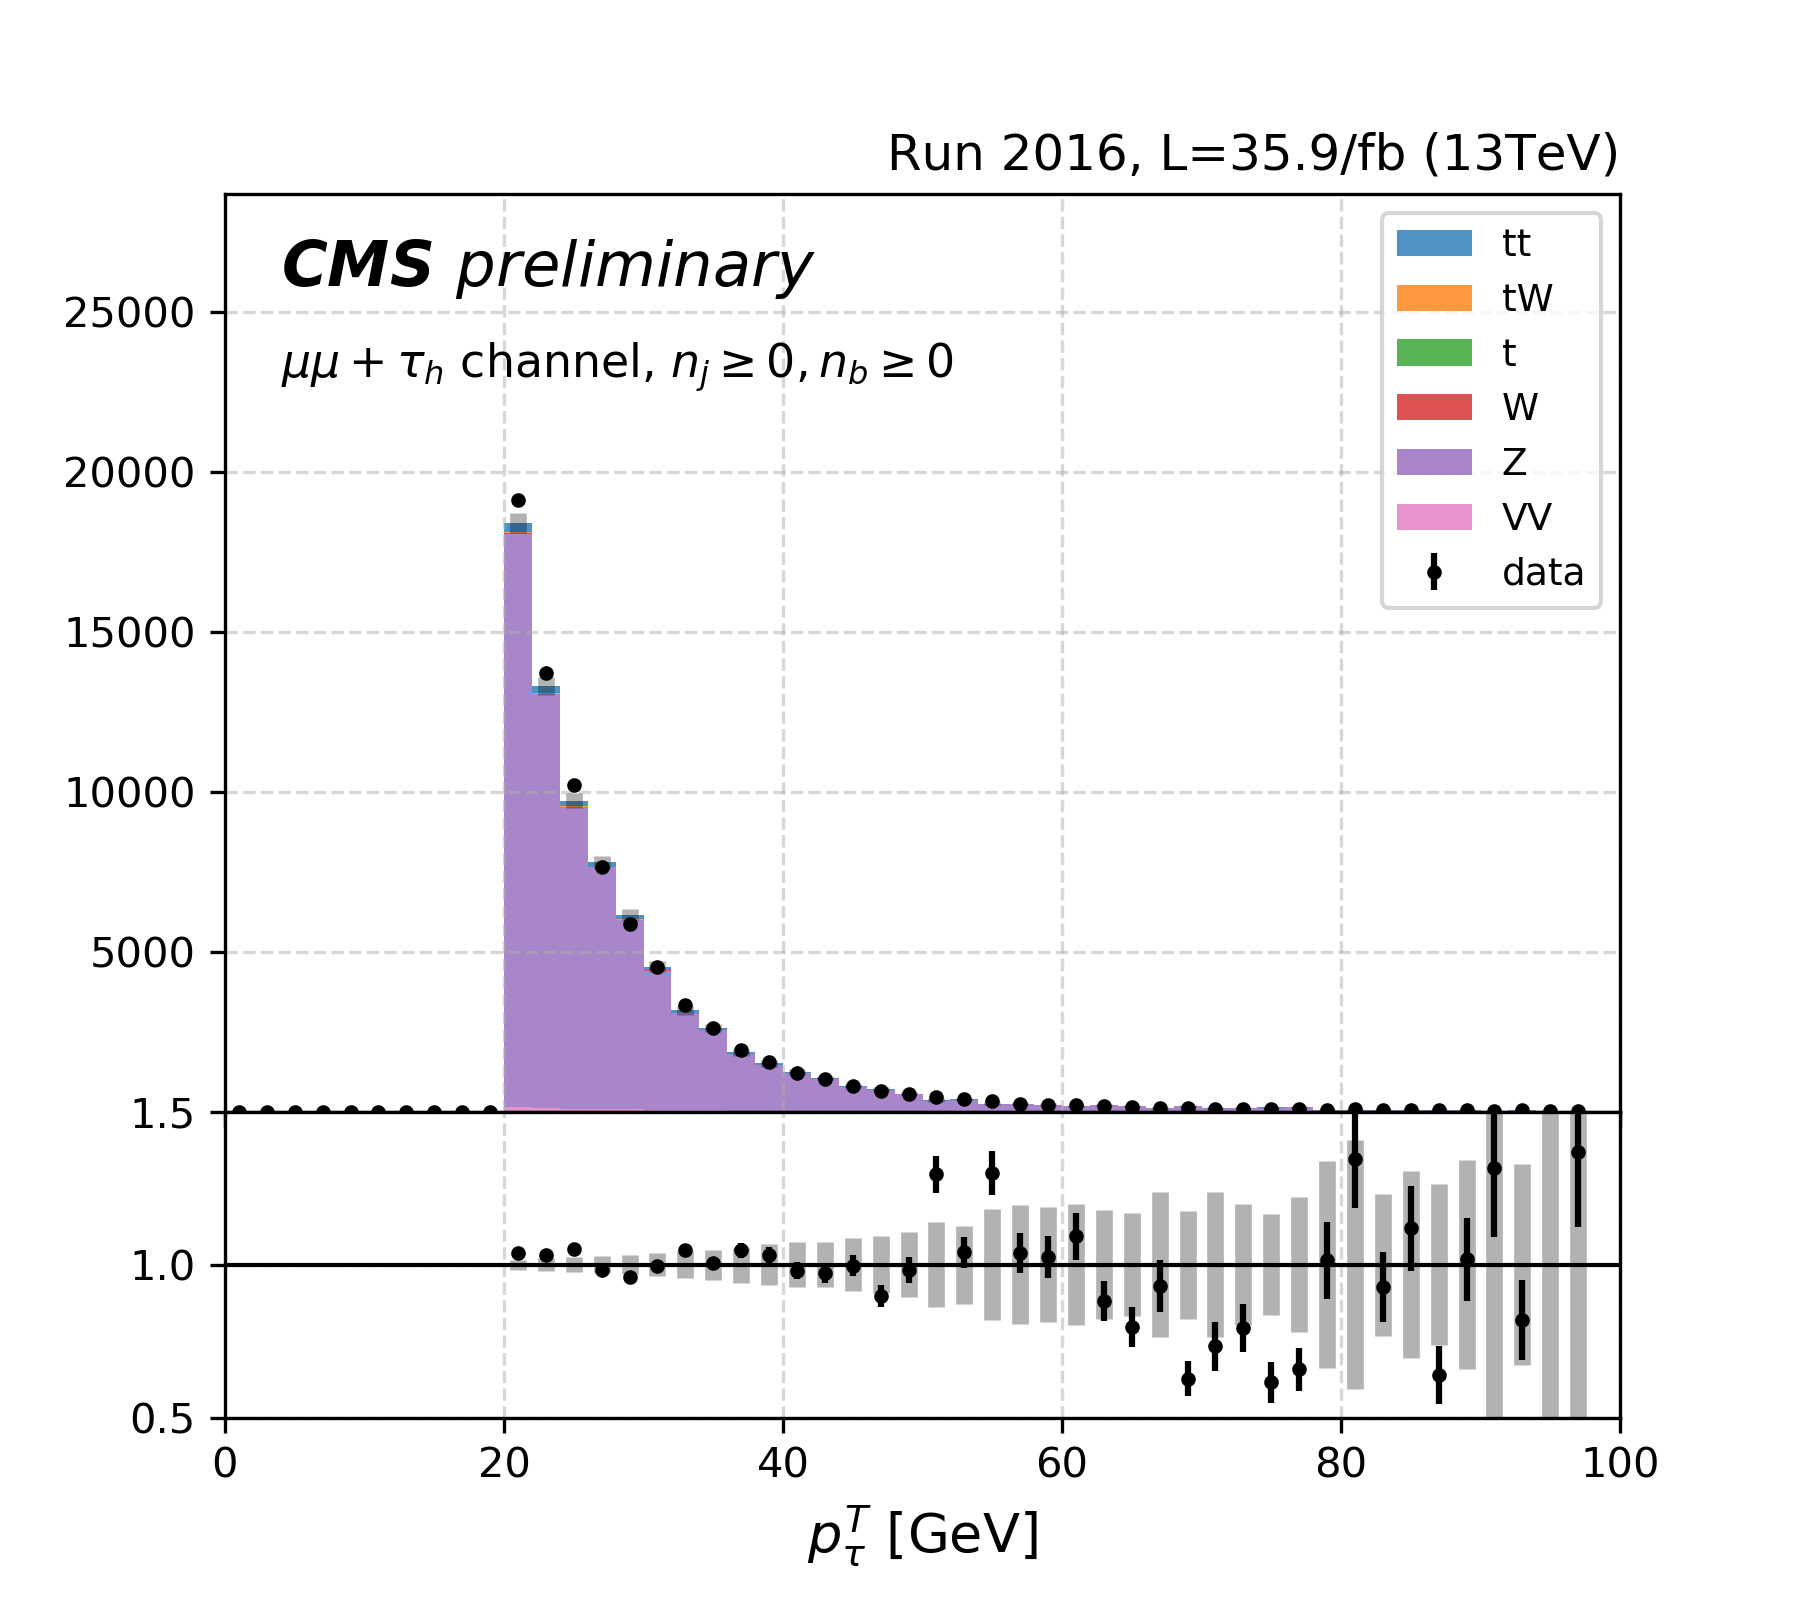
\includegraphics[width=0.32\textwidth]{chapters/Analysis/sectionCalibration/figures/jetToTauh/mumutau_tauPt_pickles_lltauTight.png}
        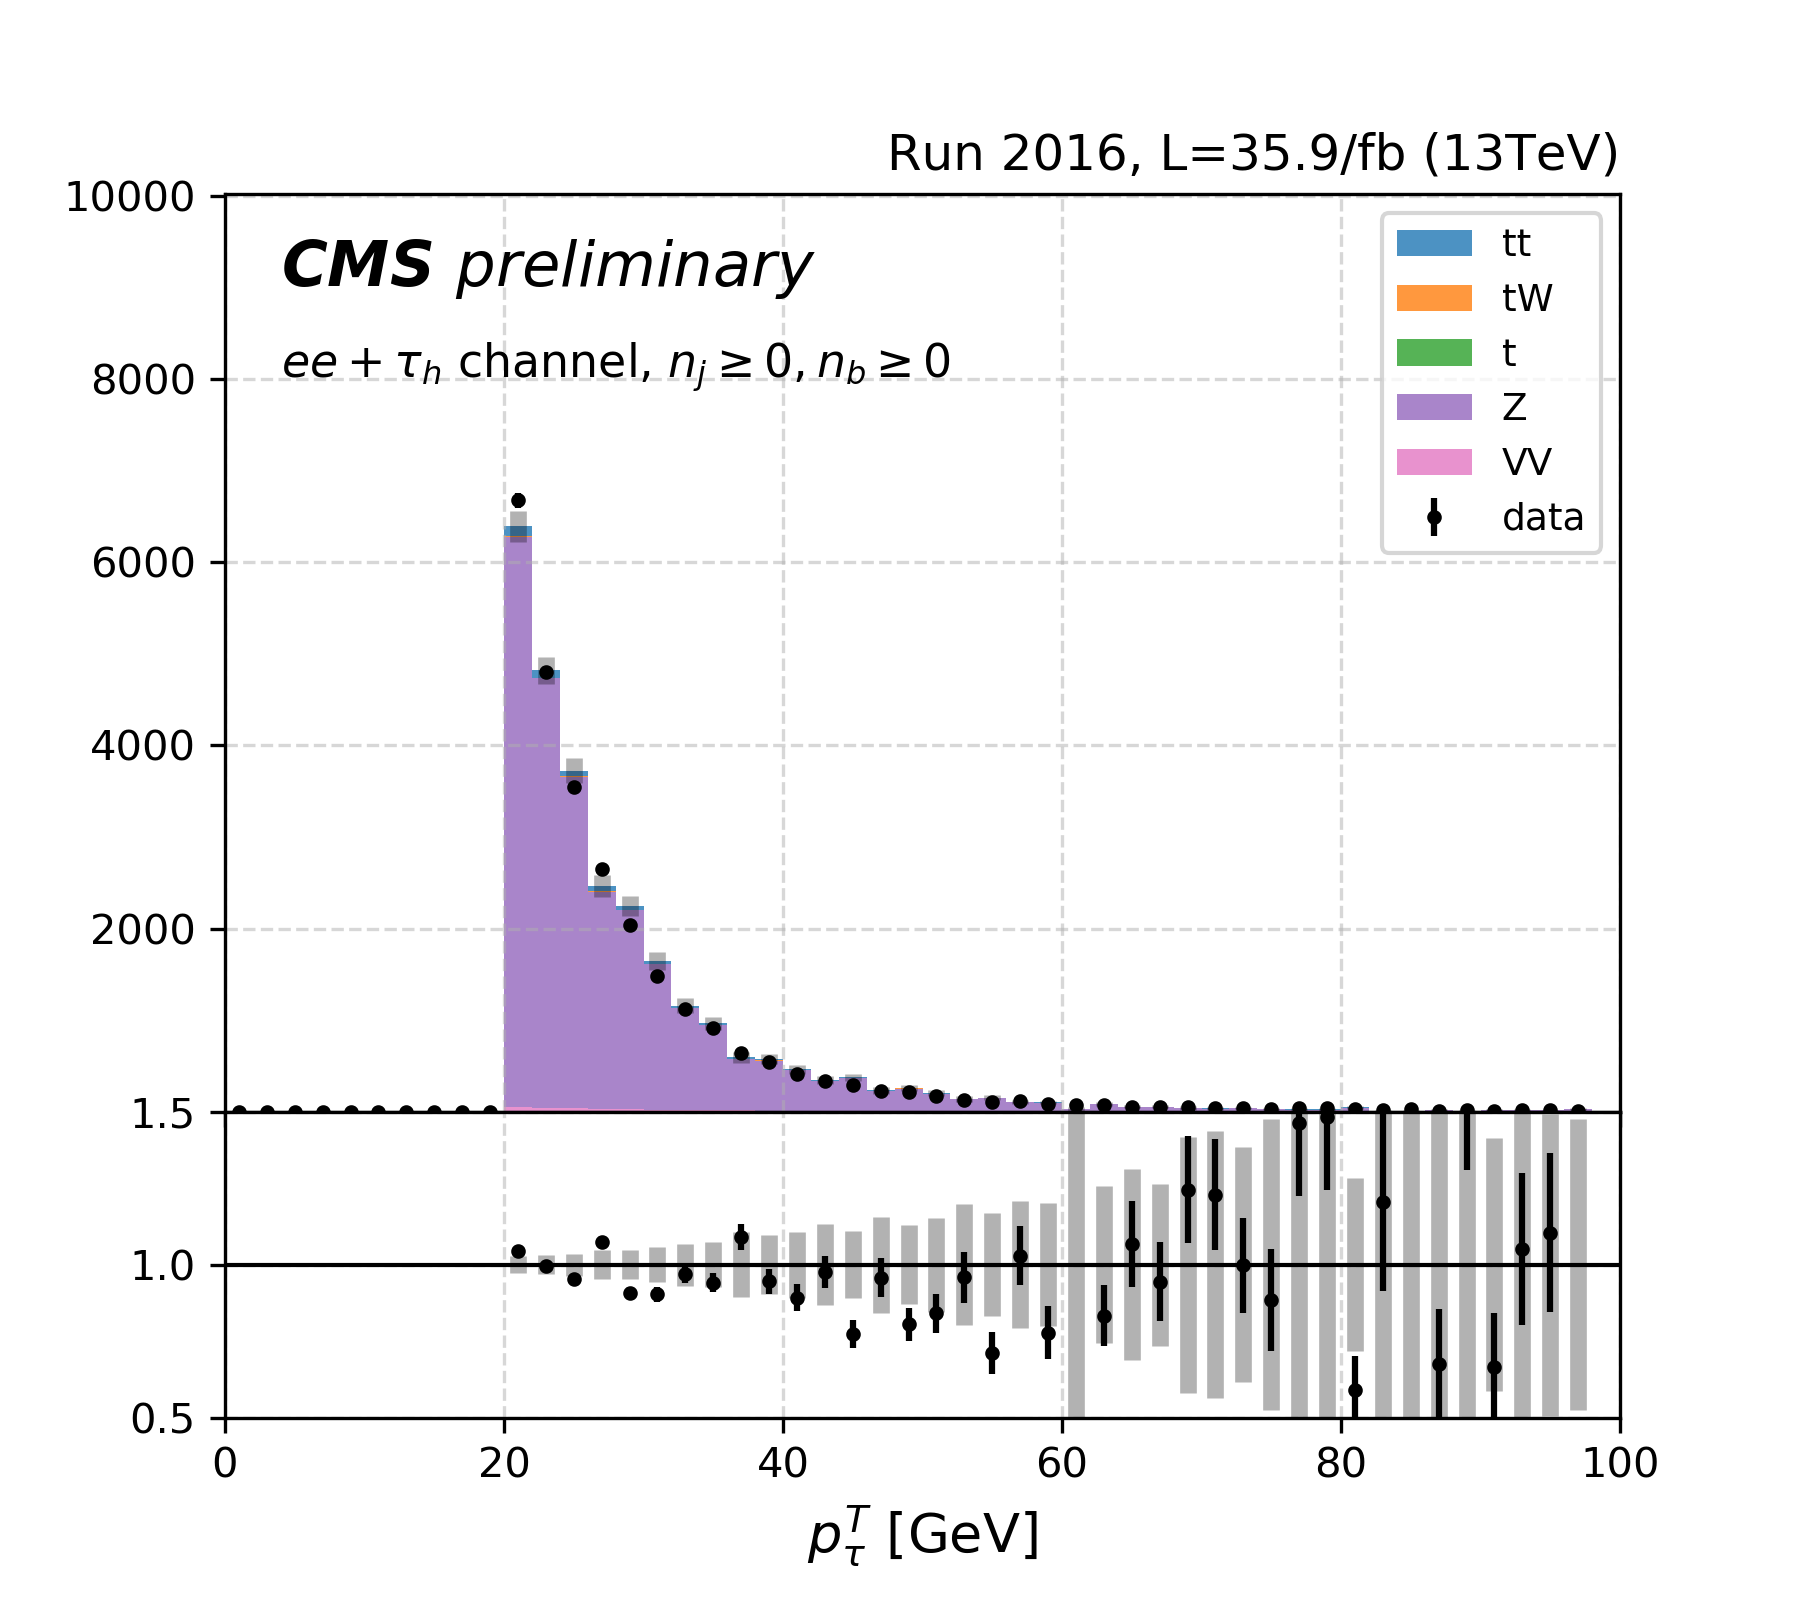
\includegraphics[width=0.32\textwidth]{chapters/Analysis/sectionCalibration/figures/jetToTauh/eetau_tauPt_pickles_lltauTight.png}
        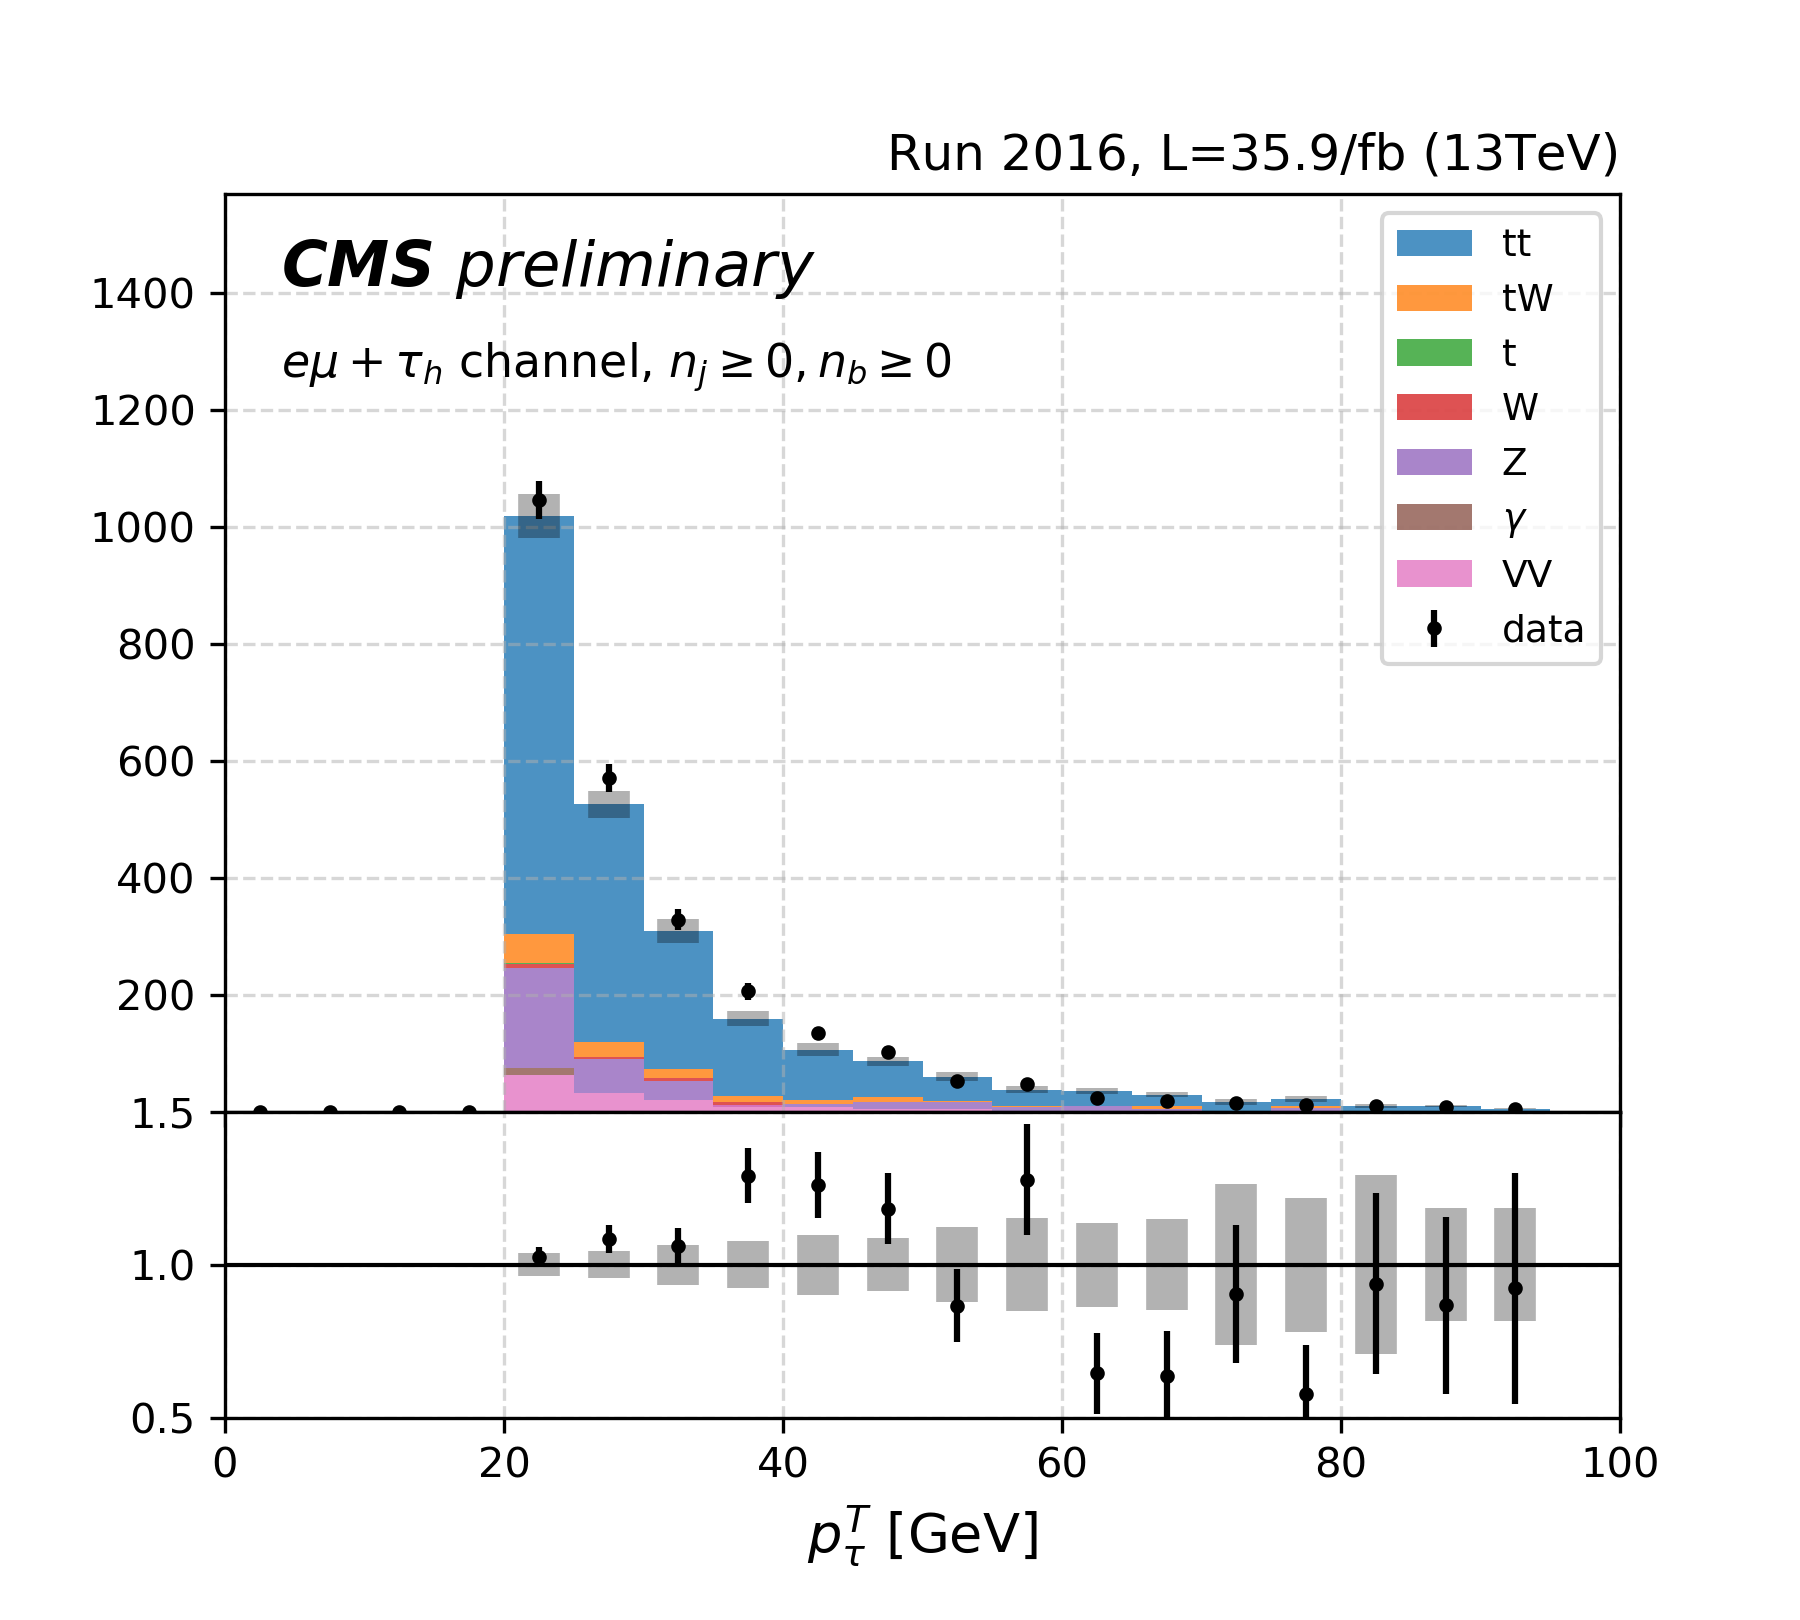
\includegraphics[width=0.32\textwidth]{chapters/Analysis/sectionCalibration/figures/jetToTauh/emutau_tauPt_pickles_lltauTight.png}
        
        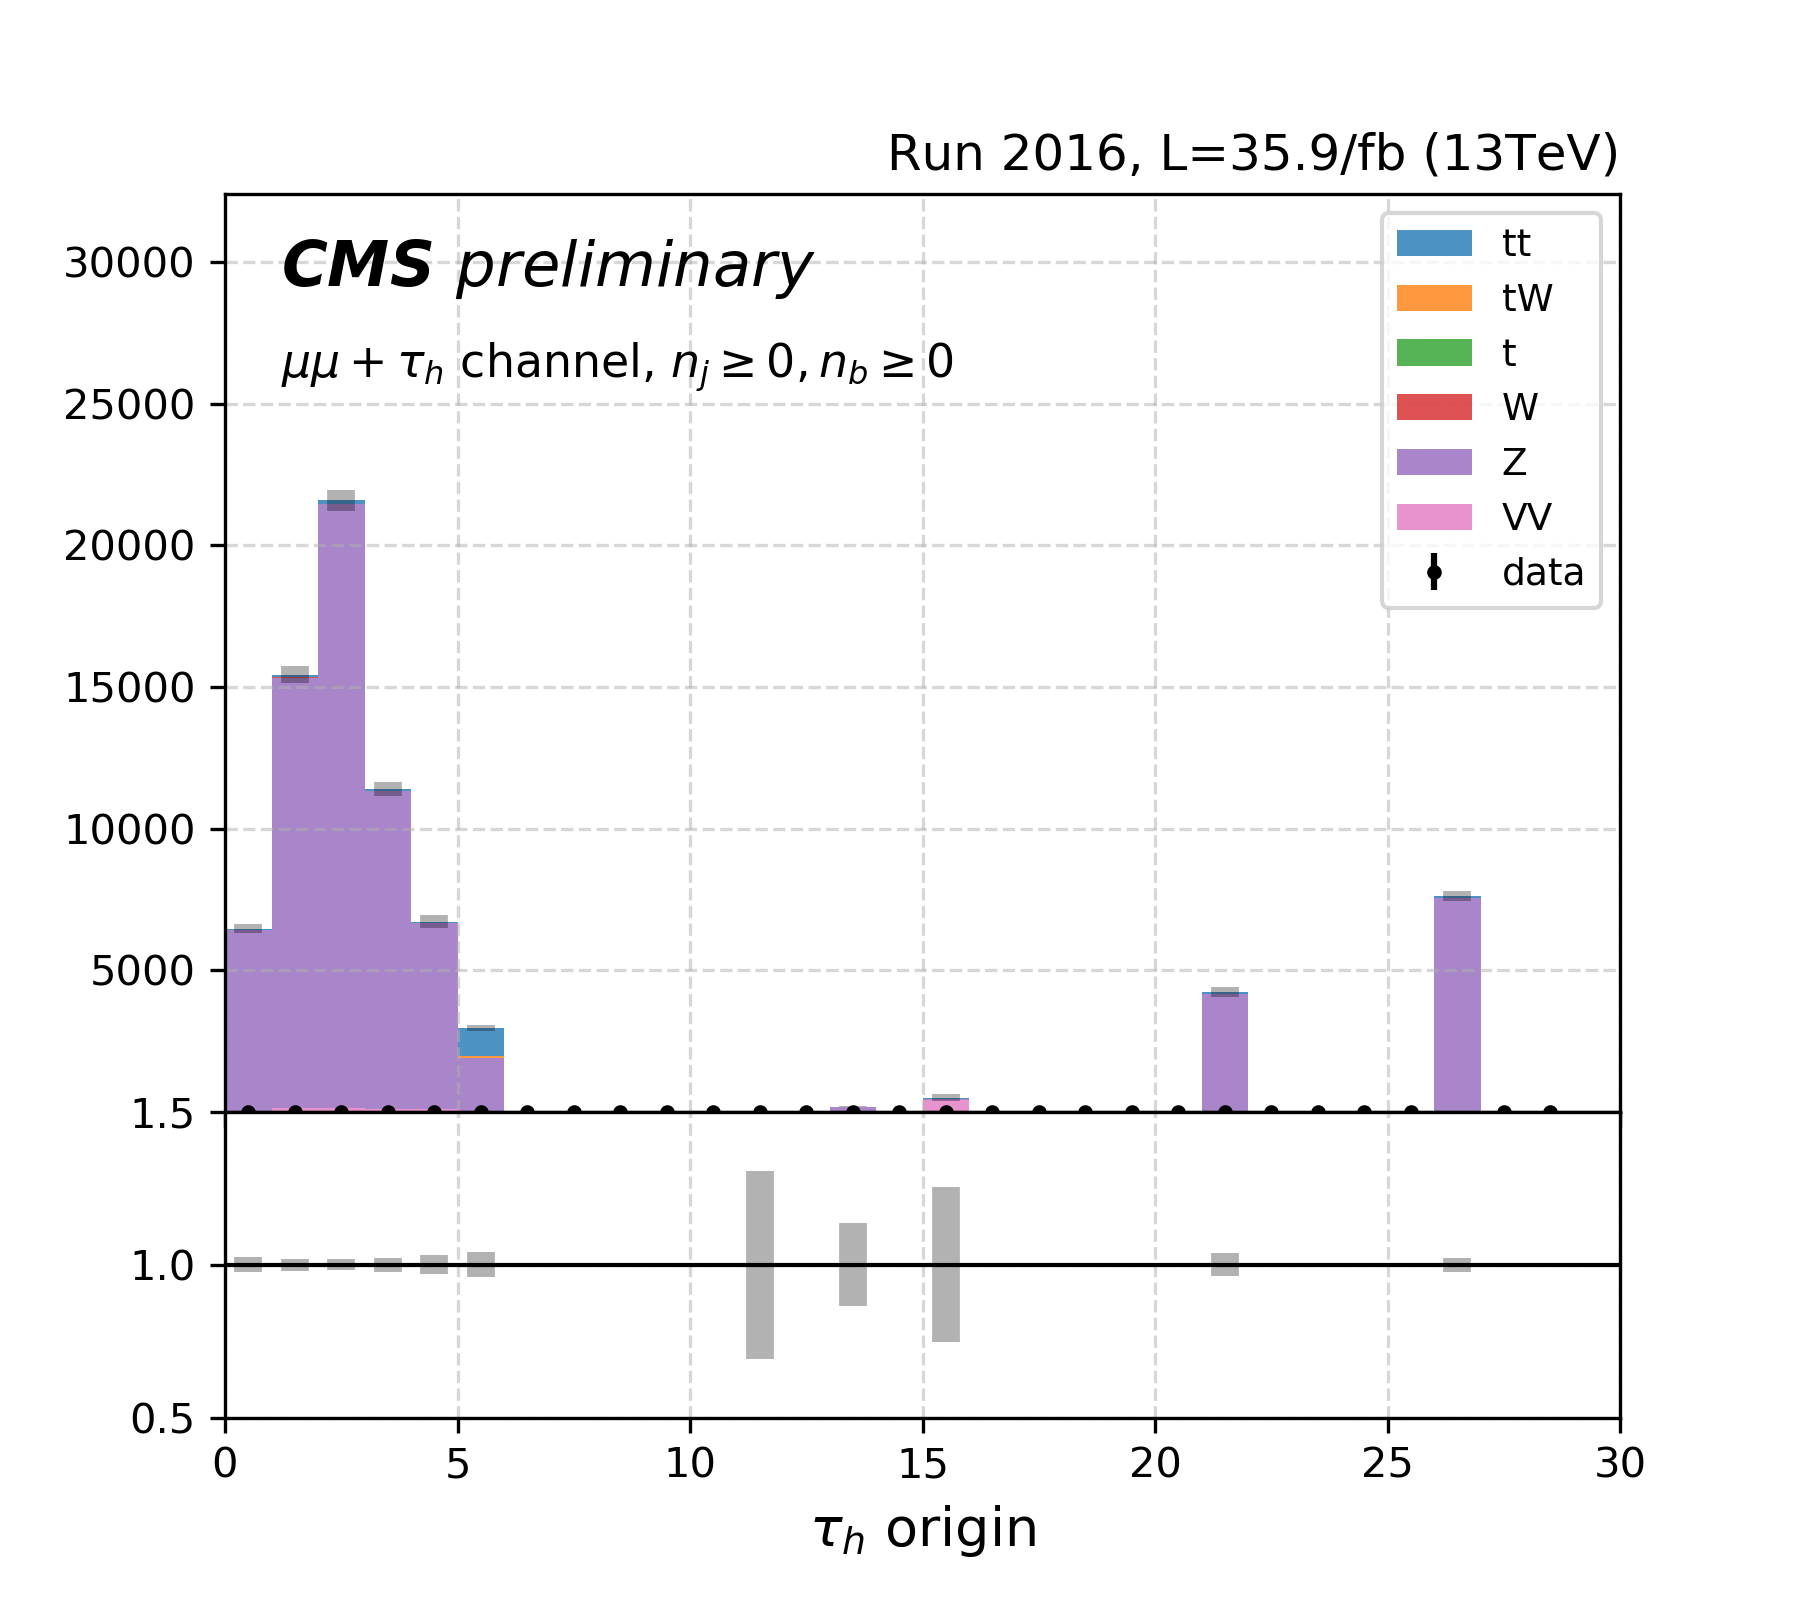
\includegraphics[width=0.32\textwidth]{chapters/Analysis/sectionCalibration/figures/jetToTauh/mumutau_tauGenFlavor_pickles_lltauTight.png}
        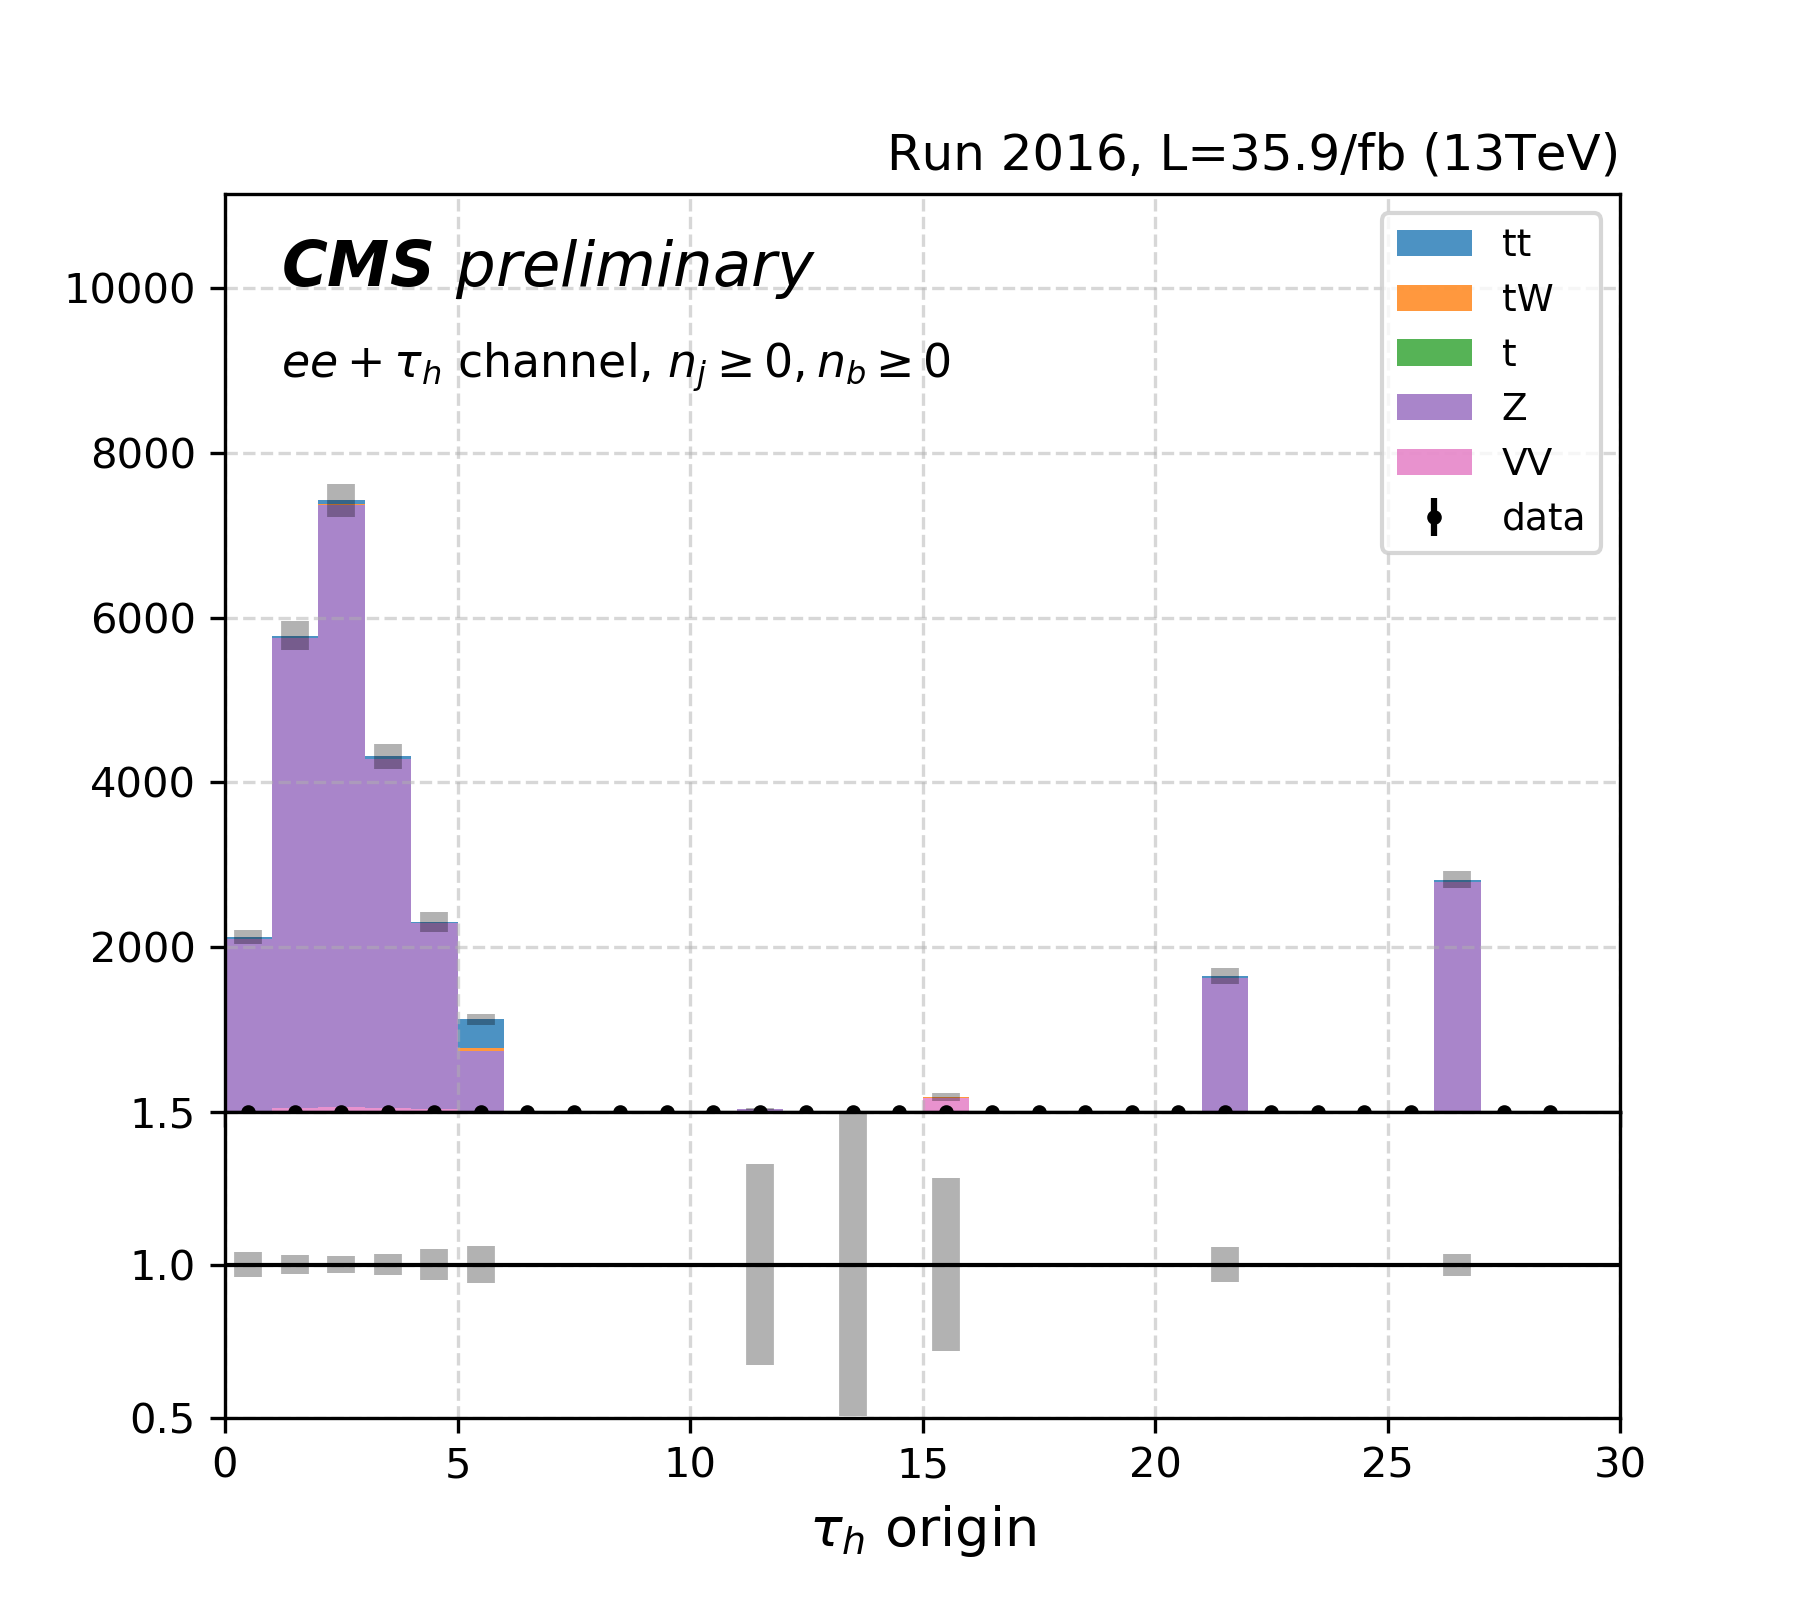
\includegraphics[width=0.32\textwidth]{chapters/Analysis/sectionCalibration/figures/jetToTauh/eetau_tauGenFlavor_pickles_lltauTight.png}
        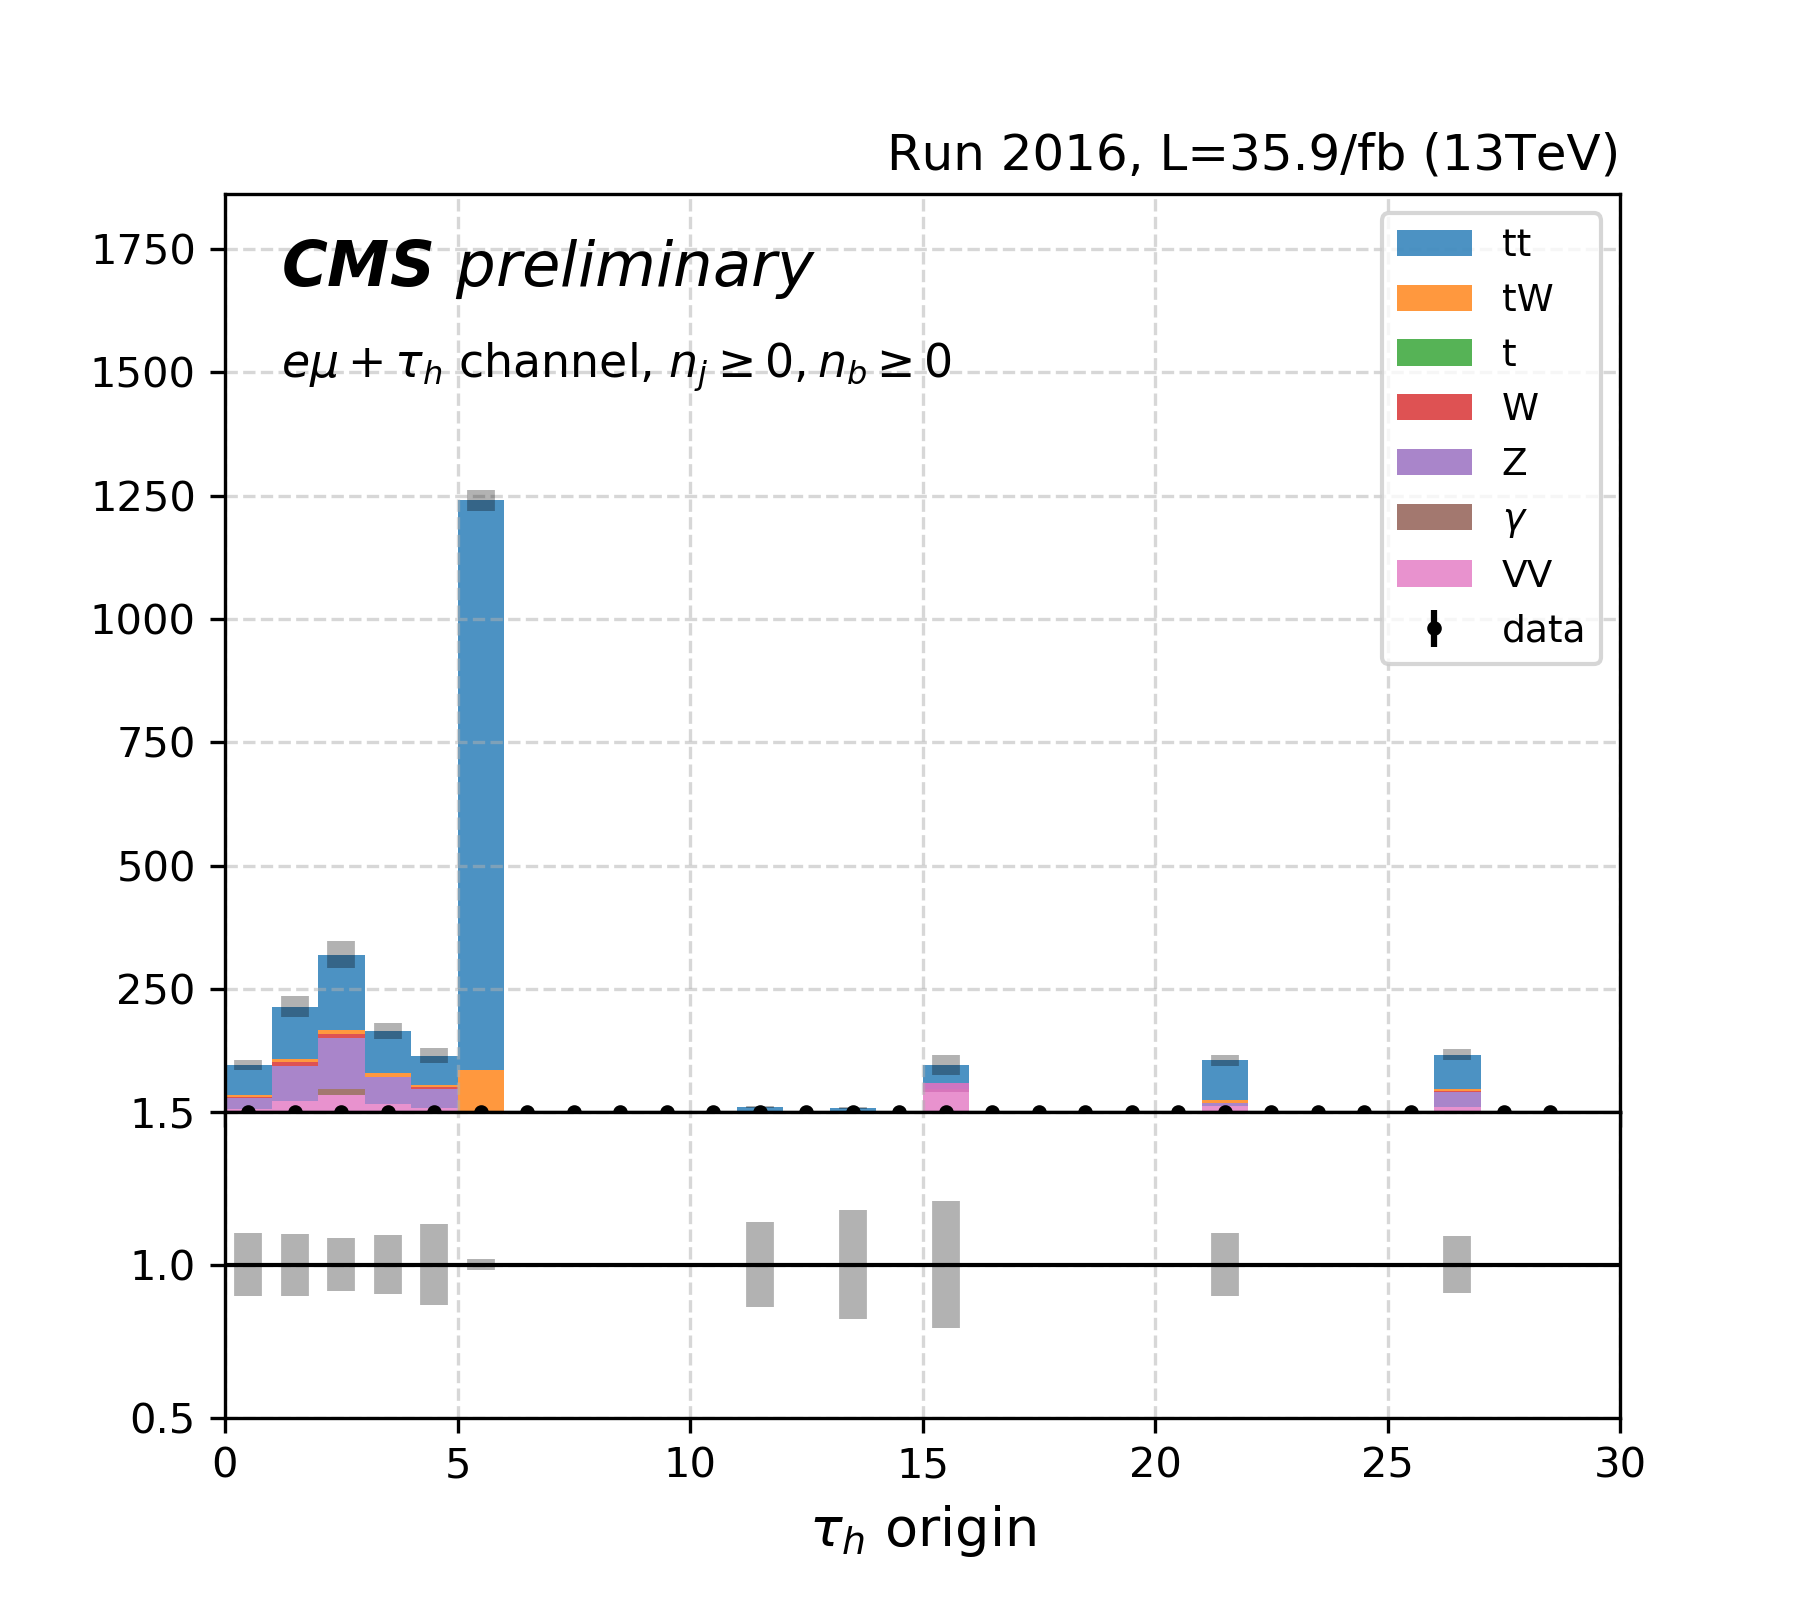
\includegraphics[width=0.32\textwidth]{chapters/Analysis/sectionCalibration/figures/jetToTauh/emutau_tauGenFlavor_pickles_lltauTight.png}
    \end{center}
\end{frame}

% -------------
% new frame
% -------------
\begin{frame}{}
\smaller
    \begin{center}
    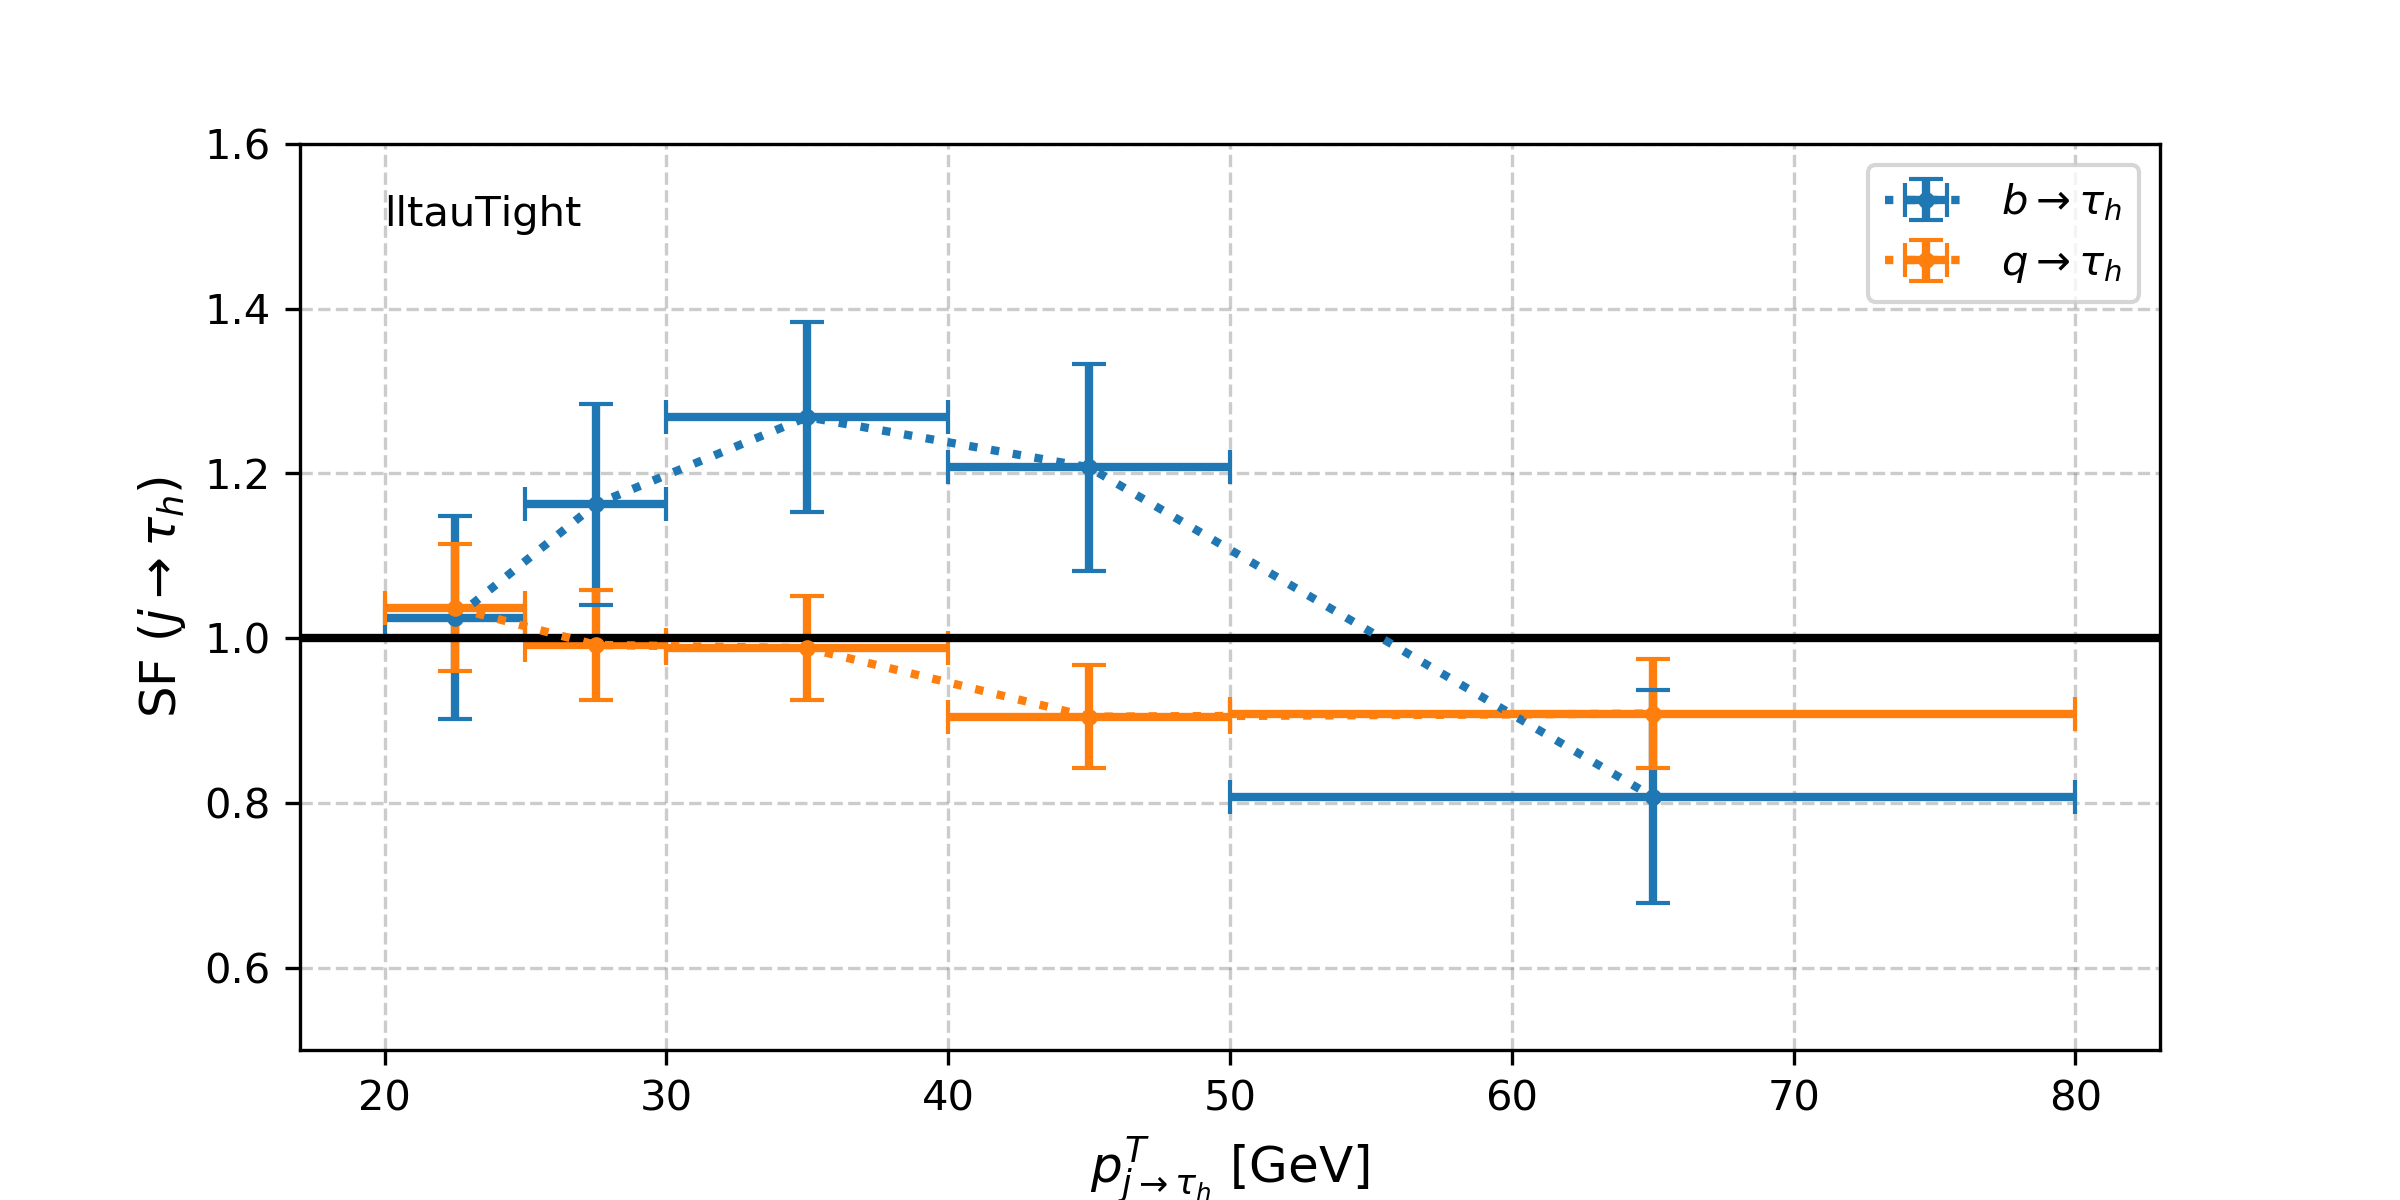
\includegraphics[width=0.49\textwidth]{chapters/Analysis/sectionCalibration/figures/jetToTauh/fit2_ptflavor2_lltauTight.png}
    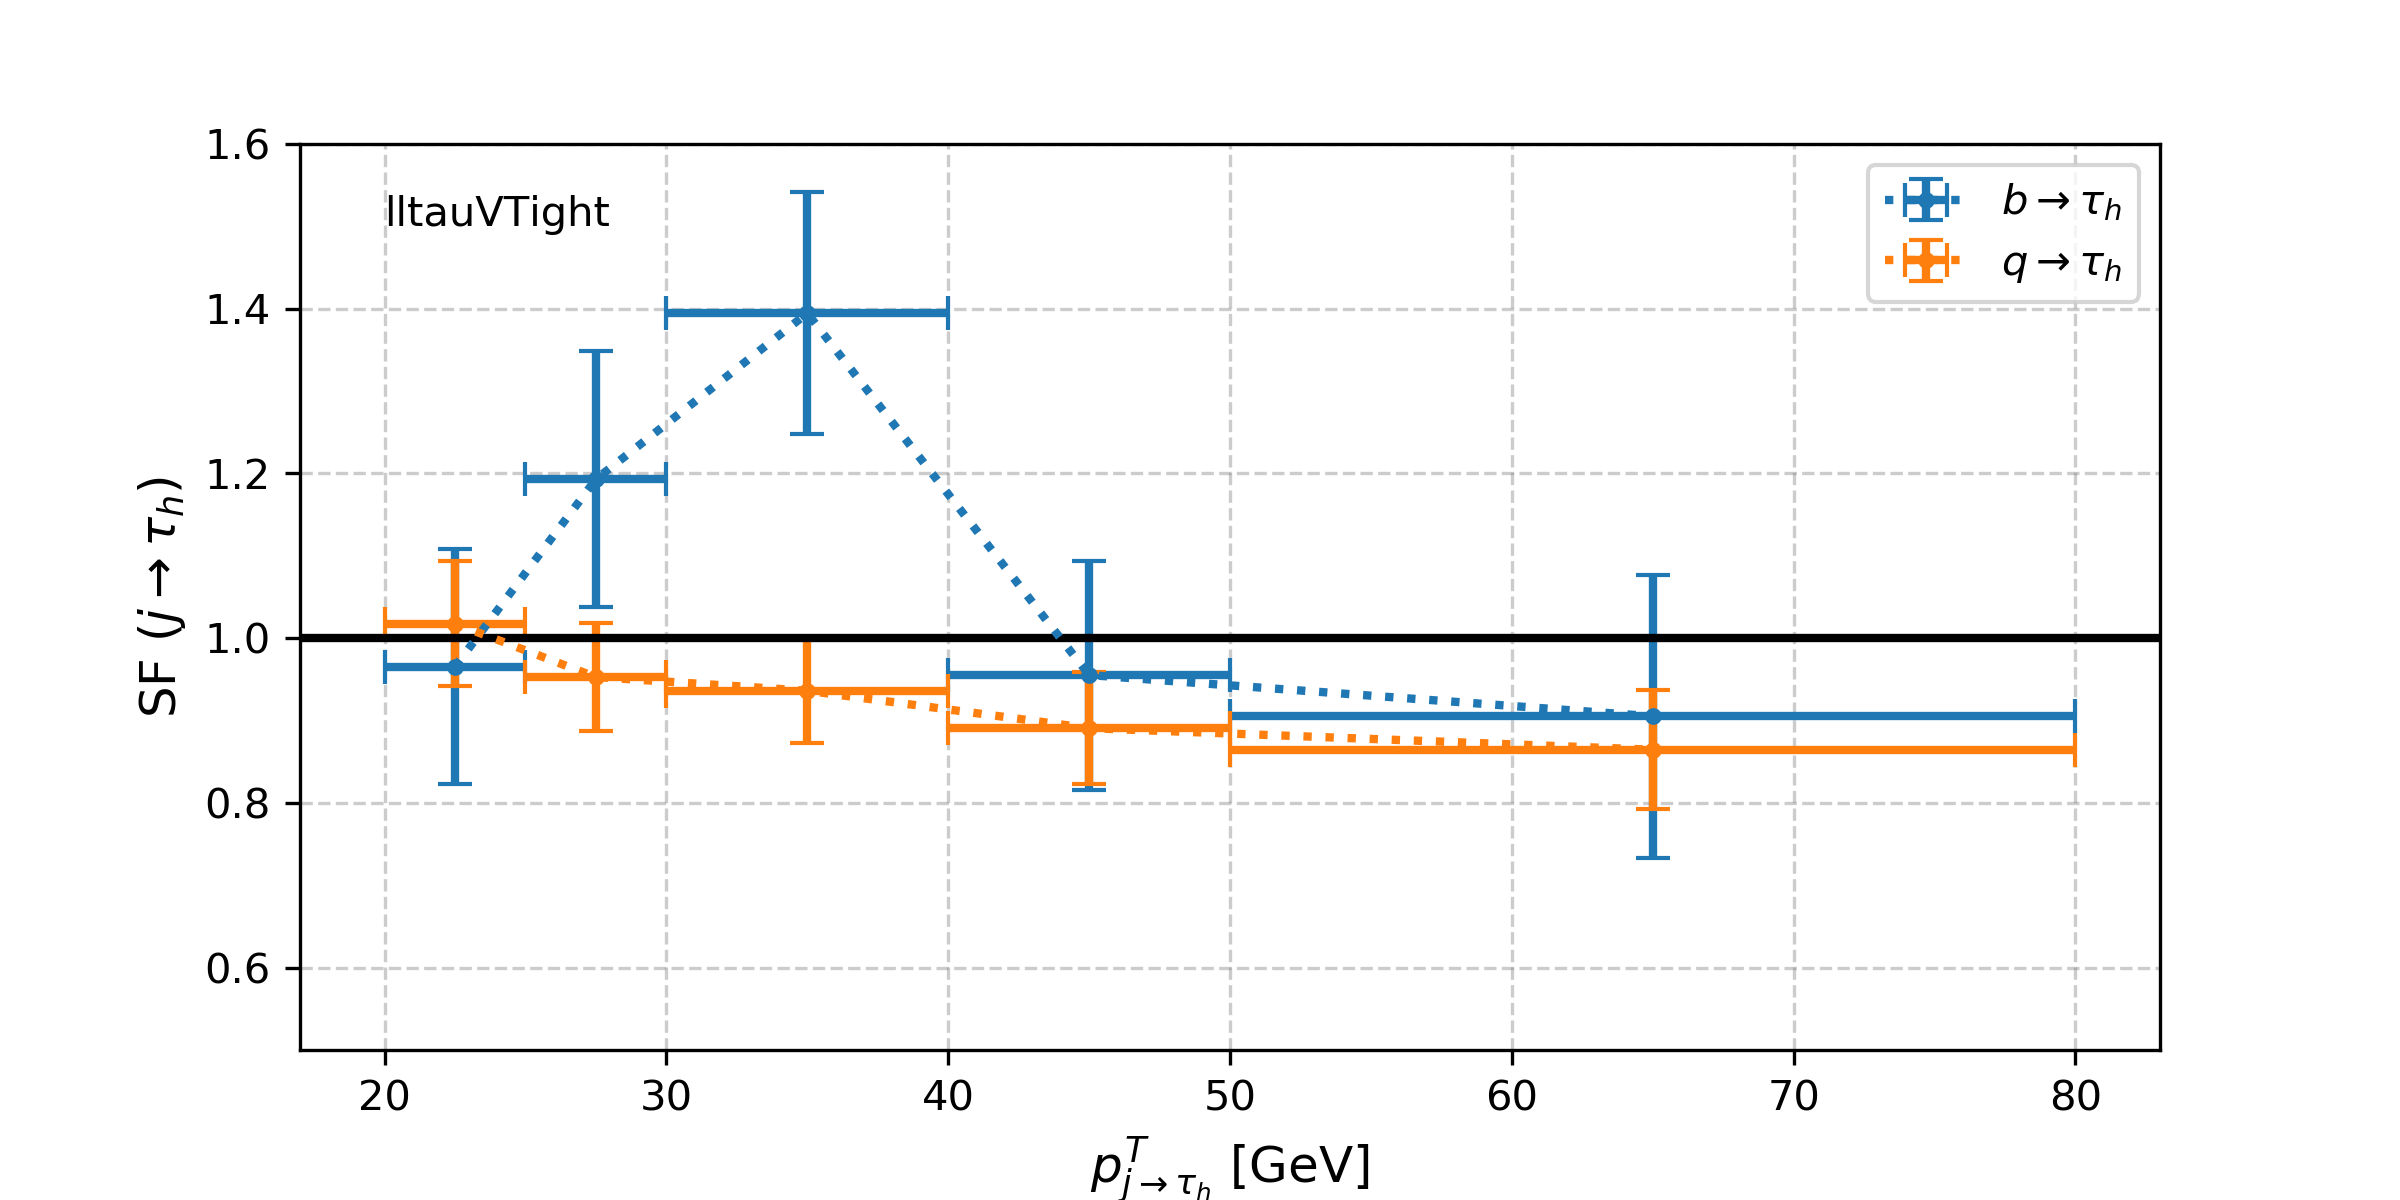
\includegraphics[width=0.49\textwidth]{chapters/Analysis/sectionCalibration/figures/jetToTauh/fit2_ptflavor2_lltauVTight.png}
    \end{center}
    
    \begin{itemize} 
        \smaller
        \item fit the \pt distribution of \PGth.
        \item free parameters for $SF_{\PQq\to \PGth}(\pt)$ and $SF_{\PQb\to \PGth}(\pt)$ in six \pt bins
        \item systematic parameters considered 
        \begin{itemize} 
            \smaller
            \item luminosity (2.5\% error)
            \item cross-sections of \ttbar (5\%), \zjets (5\%), \wjets (5\%), diboson (10\%)
            \item reconstruction efficiencies of electron (2\%) and muon (1\%)
        \end{itemize} 
        systematic parameters are Gaussian constrained w.r.t their assumed uncertainties.
    \end{itemize}
\end{frame}

% -------------
% new frame
% -------------
\begin{frame}{}
\smaller
    \begin{center}
    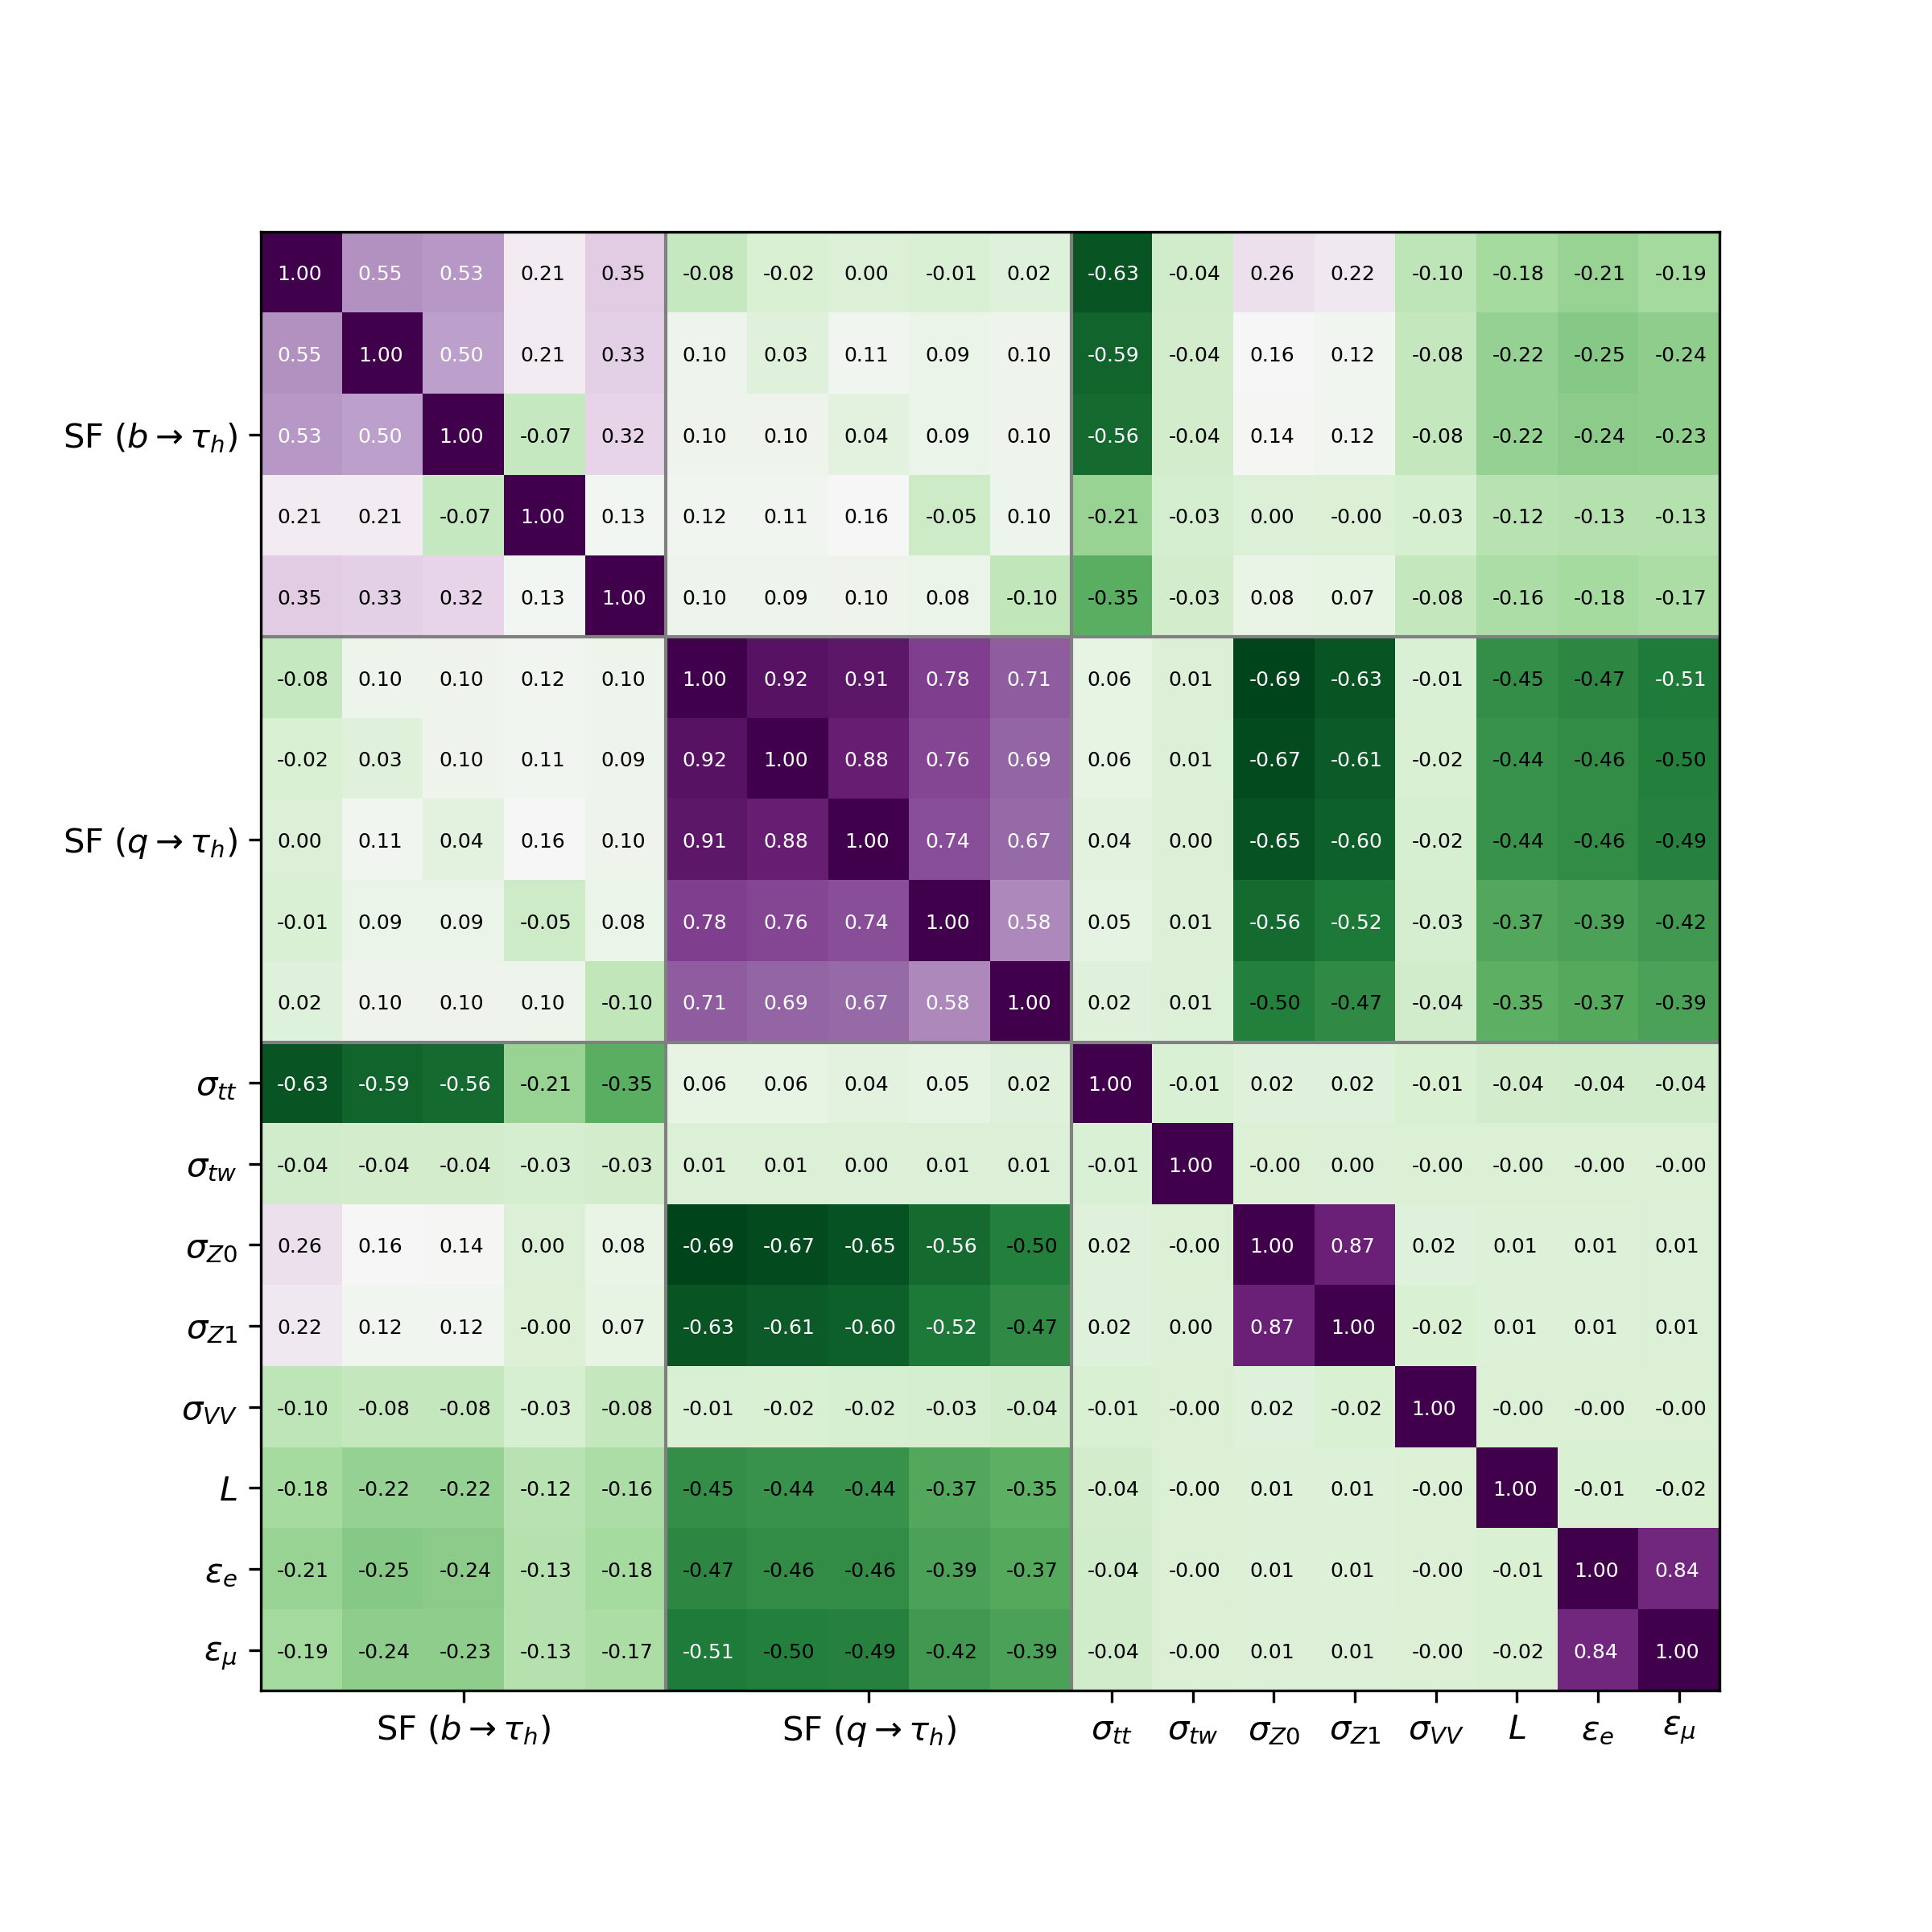
\includegraphics[width=0.4\textwidth]{chapters/Analysis/sectionCalibration/figures/jetToTauh/corr2_lltauTight_splitJetFlavor.png}
    \includegraphics[width=0.4\textwidth]{chapters/Analysis/sectionCalibration/figures/jetToTauh/corr2_lltauVTight_splitJetFlavor.png}
    \includegraphics[width=0.4\textwidth]{chapters/Analysis/sectionCalibration/figures/jetToTauh/pull2_lltauTight_splitJetFlavor.png}
    \includegraphics[width=0.4\textwidth]{chapters/Analysis/sectionCalibration/figures/jetToTauh/pull2_lltauVTight_splitJetFlavor.png}
    \end{center}
\end{frame}


\subsection{Modeling of QCD background}
\begin{frame}{Frame Title}

    \begin{center}
        \includegraphics[width=0.9\textwidth, trim=0 21cm 32cm 18cm, clip]{chapters/Analysis/sectionBackground/figures/ltau_kinematics/ltau2.png}
    \end{center}
    
    normalization from 2j0b and iso-0j0b
    \begin{equation}
    SF^{\rm SS \to OS} = \frac{N^{\rm OS}_{\rm data} - \sum N^{\rm OS}_{\rm MC} }{ N^{\rm SS}_{\rm data} - \sum N^{\rm SS}_{\rm MC} }
    \end{equation}

\end{frame}


\begin{frame}{Frame Title}

    \begin{center}
        \includegraphics[width=0.9\textwidth, trim=0 52cm 28cm 0, clip]{chapters/Analysis/sectionBackground/figures/ljets_kinematics/4j1b.png}
    \end{center}
    
    shape correction from 123j1b region
    \begin{equation}
        SF^{\rm \overline{iso} \to iso} (\pt, \eta) =  \frac{N^{\rm iso}_{\rm data} (\pt, \eta) - \sum N^{\rm iso}_{\rm MC}(\pt, \eta) } {N^{\rm \overline{iso}}_{\rm data} (\pt, \eta)- \sum N^{\rm \overline{iso}}_{\rm MC}(\pt, \eta) }
    \end{equation}

    
    \begin{center}
        \includegraphics[width=0.5\textwidth]{chapters/Analysis/sectionBackground/figures/ljets_kinematics/123j1b/SF_mu_2d.png}
    \end{center}
\end{frame}


\begin{frame}{Frame Title}
    \includegraphics[width=0.8\textwidth]{chapters/Analysis/sectionBackground/figures/ljets_application/mcNorm_ddShape.png}
    
\end{frame}






